\documentclass{aa}
%\documentclass[referee]{aa} % for a referee version
%\documentclass[preprint]{aa}
\pdfoutput=1

\bibliographystyle{aa}
%\AuthorCallLimit=200
\usepackage{booktabs}
\usepackage{csvsimple}
\usepackage{pgfplotstable}
\usepackage{array}
%\usepackage{colortbl}
\usepackage{amsmath}
\usepackage{amsfonts}
\usepackage{dsfont}
\usepackage{amsxtra}
\usepackage{hyperref}
\usepackage{amssymb}
\usepackage{upgreek}
\usepackage{comment}

\usepackage{multirow}
\usepackage{url}

\usepackage{graphicx,epsfig}
%\usepackage{dcolumn}
%\usepackage{bm}
%\usepackage{ulem}

\usepackage{xspace} 

\usepackage{color}
\usepackage{xcolor}

\usepackage{lineno}
%\linenumbers
\usepackage[export]{adjustbox}


\renewcommand{\baselinestretch}{1.2}

%\setlength{\textwidth}{17.5cm} 
%\setlength{\textheight}{24.cm}
%\setlength{\topmargin}{-1.5cm}
%\setlength{\oddsidemargin}{-0.4cm}


\newcommand{\be}{\begin{equation}}
\newcommand{\ee}{\end{equation}}
\newcommand{\bea}{\begin{eqnarray}}
\newcommand{\eea}{\end{eqnarray}}
\newcommand{\beaa}{\begin{eqnarray*}}
\newcommand{\eeaa}{\end{eqnarray*}}
\newcommand{\ba}{\begin{array}}	
\newcommand{\ea}{\end{array}}
\newcommand{\bi}{\begin{itemize}}
\newcommand{\ei}{\end{itemize}}
\newcommand{\ben}{\begin{enumerate}}
\newcommand{\een}{\end{enumerate}}

\newcommand{\bra}{\langle}
\newcommand{\ket}{\rangle}
\newcommand{\ra}{\rightarrow}
\newcommand{\lra}{\longrightarrow}
\newcommand{\overar}{\overrightarrow}
\newcommand{\wt}{\widetilde}
\newcommand{\td}{\tilde}


\newcommand{\lb}{\label}
\newcommand{\g}{\ensuremath{\gamma}\xspace}
\newcommand{\G}{\Gamma}
\newcommand{\e}{\epsilon}
\newcommand{\al}{\alpha}
\newcommand{\bt}{\beta}
\newcommand{\p}{\partial}
\newcommand{\dl}{\delta}
\newcommand{\Dl}{\Delta}
\newcommand{\ld}{\lambda}
\newcommand{\Ld}{\Lambda}
\newcommand{\vp}{\varphi}
\newcommand{\te}{\theta}
\newcommand{\Om}{\Omega}
\newcommand{\om}{\omega}
\newcommand{\sm}{\sigma}
\newcommand{\Sm}{\Sigma}

\newcommand{\A}{{\rm A}}
\newcommand{\B}{{\rm B}}
\newcommand{\U}{{\rm U}}
\newcommand{\F}{{\rm F}}
\newcommand{\SU}{{\rm SU}}
\newcommand{\Tr}{{\rm Tr}}
\newcommand{\Hom}{{\rm Hom}}

\newcommand{\FF}{{\mathsf F}}

\newcommand{\mcE}{{\mathcal{E}}}
\newcommand{\N}{{\mathcal{N}}}
\newcommand{\D}{{\mathcal{D}}}
\newcommand{\La}{{\mathcal{L}}}
\newcommand{\OO}{{\mathcal{O}}}
\newcommand{\M}{{\mathcal{M}}}


\newcommand{\mbE}{{\mathbb{E}}}
\newcommand{\Z}{{\mathbb{Z}}}
\newcommand{\R}{{\mathbb{R}}}
\newcommand{\C}{{\mathbb{C}}}
\newcommand{\NN}{{\mathbb{N}}}
\newcommand{\PP}{{\mathbb{C}}{\rm P}}

\newcommand{\HH}{{\mathcal{H}}}
\newcommand{\Hd}{{\mathcal{H}}^*}

\newcommand{\HI}{H~\textsc{i}\xspace}
\newcommand{\Htwo}{$\mathrm{H}_2$\xspace}
\newcommand{\hi}{$\mathrm{H\,\scriptstyle{I}}$\xspace}
\newcommand{\hii}{$\mathrm{H\,\scriptstyle{II}}$\xspace}
\newcommand{\hd}{$\mathrm{H}_2$\xspace}
\newcommand{\xco}{$X_\mathrm{CO}$\xspace}

\newcommand{\vx}{{\bf x}}

\newcommand{\Fermi}{\textit{Fermi}\xspace}
\newcommand{\LAT}{\textsl{LAT}\xspace}
\newcommand{\WMAP}{\textsl{WMAP}\xspace}
\newcommand{\Planck}{\textsl{Planck}\xspace}
\newcommand{\Suzaku}{\textsl{Suzaku}\xspace}

\newcommand{\SM}{Sample Model\xspace}

\newcommand{\sigmav}{\ensuremath{\langle \sigma v \rangle}\xspace}
\newcommand{\bbbar}{\ensuremath{b \bar b}\xspace}
\newcommand{\tautau}{\ensuremath{\tau^{+}\tau^{-}}\xspace}
\newcommand{\relic}{\ensuremath{2.2\times10^{-26}\cm^{3}\second^{-1}}\xspace}
\newcommand{\beff}{\ensuremath{b_{\rm eff}}\xspace}
\newcommand{\DM}{\ensuremath{\mathrm{DM}}}
\newcommand{\mDM}{\ensuremath{m_\DM}\xspace}


% local options
\newcommand{\onepic}{0.45}
\newcommand{\twocolumnwidth}{0.75}
%\newcommand{\twopic}{0.38}
\newcommand{\twopic}{0.3}
\newcommand{\twopicsp}{0.45}
\newcommand{\threepic}{0.25}
%\newcommand{\threepic}{0.18}
\newcommand{\fourpic}{0.28}
\newcommand{\twopicwca}{0.35}

\newcommand{\cmap}{_afmhot}


\newcommand{\red}{\textcolor{red}}
\newcommand{\blue}{\textcolor{blue}}
\definecolor{darkgreen}{rgb}{0.0, 0.7, 0.0}
\newcommand{\green}{\textcolor{darkgreen}}

\newcommand{\dima}[1]{\textcolor{blue}{(Dima: #1)}}


\begin{document} 



   \title{Machine learning methods for constructing \\ probabilistic \Fermi-LAT catalogs}



   \author{A. Bhat \thanks{\email{aakash.bhat@fau.de}}
          \inst{1}
          \and
          D. Malyshev \thanks{on leave of absence from NRC ``Kurchatov Institute'' - ITEP, B. Cheremushkinskaya st. 25, Moscow, Russia 117218, 
          \email{dmitry.malyshev@fau.de}}
          \inst{1}
          }

   \institute{
             Erlangen Centre for Astroparticle Physics, Erwin-Rommel-Str. 1, Erlangen, Germany
             }

   \institute{
             Erlangen Centre for Astroparticle Physics, Erwin-Rommel-Str. 1, Erlangen, Germany
             }


 
\abstract
% context heading (optional)
% {} leave it empty if necessary  
{
Classification of sources is one of the most important tasks in astronomy.
Sources detected in one wavelength band, for example using gamma rays, may have several possible associations in other wavebands or
there may be no plausible association candidates.
}
% aims heading (mandatory)
{
In this work, we aim to determine probabilistic classification of unassociated sources in the third and the fourth \Fermi Large Area Telescope (LAT) point source catalogs (3FGL and 4FGL-DR2) into two classes (pulsars and active galactic nuclei (AGNs)) or three classes (pulsars, AGNs, and other sources).
}
% methods heading (mandatory)
{
We use several machine learning (ML) methods to determine probabilistic classification of \Fermi-LAT sources.
We evaluate the dependence of results on meta-parameters of the ML methods, such as the maximal depth of the trees in tree-based classification methods and the number of neurons in neural networks.
}
% results heading (mandatory)
{
We determine probabilistic classification of both associated and unassociated sources in 3FGL and 4FGL-DR2 catalogs.
We cross-check the accuracy by comparing the predicted classes of unassociated sources in 3FGL that have associations in 4FGL-DR2.
We find that in the 2-class case it is important to correct for the presence of other sources among the unassociated ones in order to realistically estimate the number of pulsars and AGNs.
In particular, the estimated number of pulsars in the 3FGL (4FGL-DR2) catalog is 270 (481) in the 2-class case without corrections for the other sources and 158 (214) in the 3-class case.
Provided that the number of associated pulsars is 167 (271) in the 3FGL (4FGL-DR2) catalog,
the number of pulsars among the unassociated sources is expected to be similar or larger than the number of associated ones. 
}
% conclusions heading (optional), leave it empty if necessary 
{}

\keywords{Methods: statistical --
                Catalogs --
                Gamma rays: general
                %Galaxy: halo --
                %Galaxy: structure -- 
                %ISM: jets and outflows
               }

\maketitle
   
   
\tableofcontents


\section{Introduction}

Multiwavelength association of astronomical sources is important for understanding their nature.
Unfortunately, in many cases a firm association of sources at different wavelength is not possible.
For example, about one third of gamma-ray sources in Fermi-LAT catalogs are unassociated.
It is useful to know at least to which class the unassociated sources belong to or, which is more typical,
what are the probabilities for the source to belong to different classes.
In this paper we use different machine learning algorithms to find probabilistic classification of
unassociated sources in \Fermi-LAT 3FGL \citep{2015ApJS..218...23A} and 4FGL \citep{2020ApJS..247...33A} catalogs.
We will refer to the catalogs, where the classification of the sources is given by probabilities as probabilistic catalogs.
In general, the classes may include the possibility that a source is not a real source but a fluctuation of a background 
or that a source is an overlay of two sources etc.
All these possibilities can be included in the probabilistic catalogs, which were previously introduced for optical sources 
\citep[e.g.,][]{2010EAS....45..351H, 2013AJ....146....7B}
and for gamma-ray sources \citep{2017ApJ...839....4D}.
Bayesian association probabilities were also introduced in the 4FGL catalog \citep{2020ApJS..247...33A} for faint sources.
Previous classification of unassociated \Fermi-LAT sources using machine learning methods include 
The goal of this paper is to construct probabilistic classification of sources in the 3FGL and 4FGL catalogs using ML algorithms.
Previously most probable classes of unassociated sources in Fermi LAT catalogs were reported in
[Saz-Parkinson etc.].
In this work we report not only the most probable classes but rather probabilities of classes using four different ML algorithms.

Catalogs of gamma-ray point sources are typically designed to have low false detection rate. 
Nevertheless, 469 sources out of 3033 in the third \Fermi-LAT catalog (3FGL) [3FGL] have no counterparts 
in the forth \Fermi-LAT catalog (4FGL) [4FGL].
This is much larger than the expected false detection rate in 3FGL arising from statistical fluctuations.
For the majority of sources in 3FGL without counterparts in 4FGL the problem is not the false detection, 
but rather the association.
For example, some sources can be detected due to deficiencies in the Galactic diffuse emission model.
In this case, the statistical significance of the detection is high, but the association is wrong: the sources should be classified as
a part of the Galactic diffuse emission rather than point-like sources.
Another reason could be that two (or more) point-like sources in 3FGL are associated to a single extended source in 4FGL,
or a single source is resolved into two sources.
Again, this is a problem of classification (or association) rather than false detection.

Another reason for an absence of a previously detected source in a new catalog is variability.
In particular, flat spectrum radio quasars (FSRQs) are highly variable active galactic nuclei (AGNs).
If a source was active during the observation time of 3FGL but inactive afterwards, 
then its significance in the 4FGL can be below the detection threshold.
The problem here is connected to a selection of a hard detection threshold of $TS = 25$ for 3FGL and 4FGL catalogs.
Selection of a lower detection threshold could help to keep the variable sources inside the catalog, 
but it will not solve the problem, since the variable sources near the lower threshold can also disappear in the new catalog.
Moreover, lower threshold would lead to more false detections due to fluctuations of the background.
Thus, on the one hand, lower threshold can be useful in studies, where a more complete list of sources is desirable,
while the higher false detection rate is admissible. On the other hand, lower threshold can be problematic for studies where 
a clean sample is necessary. 

The problems of the miss-classification of the sources and the detection threshold can be ameliorated
with the development of a probabilistic catalog.
In this catalog, each point-like object detected above a certain threshold
is classified into several classes with a set of probabilities, rather than associated to one class (or deemed unassociated).
The classes can be various types of Galactic and extra-galactic sources, diffuse emission deficiency, extended source.
Even the statistical fluctuation of the background can be viewed as one of the classes: in this case, objects with small statistical significance
will have a high probability to be associated to the statistical fluctuation class.
A user of such a catalog will have the freedom to choose the probability threshold for the class that he or she is interested in.








\begin{comment}
False detections may arise, for example, from statistical fluctuations of the background emission, from deficiencies in the diffuse emission model, or from an overlap of faint sources, which results in a detection of a single source.
The low false detection rate is achieved by setting a high statistical significance threshold, e.g., 4 or 5 sigma.
Although a high detection threshold helps to eliminate most of the false detections due to statistical fluctuations, it is not very effective against deficiencies of the background model or overlapping sources. 
Moreover, a high threshold removes many objects, which have a high chance to be point-like sources.
%In some problems including more sources with a higher contamination is beneficial, for example, in correlating gamma-ray PS with astrophysical neutrinos or in cross-correlation of the distribution of gamma-ray sources and large scale structures at different redshifts.
In other words, the catalogs are typically designed to be clean, but in some cases one may be interested to have a complete catalog. For example, one may want to have a list of all possible pulsar candidates among the unassociated sources in a catalog, which can be derived at the expense of many non-pulsars in the list.


The idea of probabilistic catalogs [Finkbeiner] is to include additional information, which describes a probability that a particular object is a point source or that a particular unassociated PS belongs to a certain class. 
%The probabilistic catalog can be implemented at the level of the PS detection, or it can also be implemented at the level of associations of already detected PS. 
For example, about one third of \Fermi-LAT sources have no firm associations with known Galactic or extragalactic sources. 
Although the associations are unknown, these sources can still be classified with some probabilities into, e.g., extragalactic or Galactic sources based on their position on the sky, properties of the gamma-ray flux and other features.
The classes can be further subdivided into various types of blazars or galaxies for extragalactic sources, or pulsars, pulsar wind nebulae, or supernova remnants for Galactic sources.
The classification probability is not unique, it depends on the classification method. The range of probabilities corresponding to different methods can serve as an estimate of the modeling uncertainty of the classification. In case of PS detection, one can derives probabilities that an object is a point source, a statistical fluctuation of the background, a deficiency of the background model, or an overlap of point sources. 
In this case, the probability will include not only the statistical probability but also the modeling uncertainties.

\end{comment}



In this paper we construct a probabilistic catalog using, as an example, classification of unassociated sources in \Fermi-LAT catalogs. 
We start with the 3FGL catalog and classify the unassociated sources into pulsars and AGNs using the associated sources in 3FGL for training of the classification algorithms.
We use several machine learning algorithms for the classification, e.g., random forest, boosted decision trees, logistic regression,
and neural networks.
We show applications of the probabilistic catalog for predicting the number of pulsars and AGNs among the unassociated source and in construction of the source counts as a function of their flux, $N(S)$.
Since unassociated sources on average have smaller flux than the associated ones, 
we expect that the $N(S)$ distribution for unassociated sources has a more important contribution to the total expected number of sources
for smaller fluxes compared to counting only the associated sources.
We compare the predictions for the $N(S)$ functions based on the 3FGL catalog with the 4FGL catalog.
We also probabilistically classify unassociated sources in the 4FGL catalog.



\section{Choice of methods}
\lb{sec:methods}

\subsection{General methodology}

The first choice one has to make in constructing a probabilistic catalog is the input data and the machine learning methods.
For the input data we take associated point sources (PS) in the 3FGL catalog, which we split into training and testing subsets.
We consider four machine learning algorithms: random forests \citep[RF,][]{709601, Breiman:2001hzm}, 
boosted decision trees \citep[BDT,][]{friedman2001},  
logistic regression \citep[LR,][]{cox1958}, 
and neural networks \citep[NN,][]{Hopfield:1982pe}.
Although the performance of algorithms on testing data is slightly different, 
we report the classification probabilities for all four algorithms.
The difference among the predictions will serve as a measure of modeling uncertainty related 
to the choice of the classification algorithm.

\subsection{Discussion of the choice of the classification algorithms}
\lb{sec:class_alg}


One of the most simple and transparent algorithms for classification is decision trees.
In this algorithm, at each step the sample is split into two subsets using one of the input features.
The choice of the feature and the separating value are determined by minimizing an objective function, such as misclassification
error, Gini index, or cross-entropy.
This method is very intuitive, since at each step the results can be described in words, 
for example, at the first step, the sources can be split in mostly Galactic and extragalactic by a cut on the Galactic latitude.
At the next step, the high latitude sources can be further subsplit into millisecond pulsars and other sources, by a cut on the spectral index around 1 GeV (pulsars have a hard spectrum below a few GeV) etc.
One of the problems with decision trees is either overfitting or bias: if a tree is too deep, then it will pick up particular cases of the training sample resulting in overfitting, while too shallow trees would not be able to describe the data well, which can lead to bias. 
As a result, one needs to be very careful in selecting the depth of the tree.
This problem can be avoided if a random subset of features is used to find a division at each node. This is the basis of the RF algorithm,
where the final classification is given by an average of several trees with random subsets of features used at each node.
Another problem with the simple trees is that it can miss the classification of some subsets of data. In BDT algorithms, the final classification is given by a collection of trees, where each new tree is created by increasing the weights of misclassified samples of the previous step. 
Finally, simple trees predict classes for the data samples, while we would like to have probabilities of classes (also known as soft classification).
RF and BDT algorithms, by virtue of averaging, provide probabilities. As a result, we will use RF and BDT algorithms rather than simple decision trees in this paper.

Tree-based algorithms, even after averaging in RF and BDT methods, have sharp edges among domains with different probabilities.
In LR algorithm, the probabilities of classes are by construction smooth functions of features.
In particular, for two-class classification the probability of class 1, given the set of features $x$, is modeled by sigmoid (logit) function
\bea
\lb{eq:logit}
p_1(x) = \frac{e^{m(x)}}{1 + e^{m(x)}}.
\eea
The probability of class 0 is then modeled as $p_0(x) = 1 - p_1(x)$.
If $m(x)$ is a linear function of features, then the boundary between the domains, defined, e.g., as $p_1(x) = 0.5$, will be linear
at $m(x) = 0$.
More complicated boundaries can be modeled by taking non-linear functions $m(x)$.
Unknown parameters of the function $m(x)$ are determined by maximizing the log likelihood of the model given the known classes of the data in the training sample.
A useful feature of the LR method is that it, by construction, provides probabilities of classes with smooth transitions among domains of different classes.
A limitation is that the form of the probability function is fixed to the sigmoid function in Eq. (\ref{eq:logit}).

We notice that if $m(x)$ is a linear function of features $x$, then the LR model is obtained by an application of sigmoid function to a linear combination of input features.
This is in fact a single layer perceptron, or a NN, with several input nodes (each node corresponds to a feature) and one output node, which corresponds to $p_0(x)$, but without any hidden layers.
The output value is obtained by a non-linear transformation (sigmoid) of a linear combination of features.
Neural network with several hidden layers is obtained by a sequence of non-linear transformations of linear combinations of features.
In particular, the values in the first hidden layer are obtained by a non-linear transformation of linear combinations of input features.
Then the values in the second hidden layer are obtained by a non-linear transformation of linear combinations of values in the first hidden layer etc.
In the context of neural networks, the non-linear transformations are called activation functions.
If the activation function for the output layer is sigmoid, then the output value (values) can be interpreted as probabilities.


\section{Construction of probabilistic catalogs}
\lb{sec:training}

One of the first problems, one has to deal with for the 3FGL and 4FGL-DR2 catalogs, is that
some of the sources in the catalogs have missing or unphysical values (e.g., infinity).
In order to avoid a bias in predictions, we include sources with missing or unphysical values only in testing or in predictions (for unassociated sources), but not in training.
If the value is infinity, then we formally substitute it by the largest value found in the samples multiplied by 10.
An unphysical zero (e.g., in significance) is substituted by the smallest value in the sample divided by 10,
while a missing value is substituted by the average in the sample.
There can be other ways to replace the missing or unphysical values, e.g., by using k nearest neighbors regression, 
but since the number of such sources is relatively small (13 for 3FGL and 14 for 4FGL-DR2), 
the choice of the method to replace the missing values does not significantly affect the results.
In the final probabilistic catalogs, we use a column ``Missing\_Values\_Flag'' to mark sources with missing or unphysical values.

As an example of the construction of a probabilistic catalog, we will use the 3FGL catalog.
In this section we will perform a two-class classification to separate PS into pulsars and AGNs.
Thus for training and testing, we subselect the sources, which are associated to pulsars and AGNs
(three-class classification into pulsars, AGNs, and other sources is discussed in Section \ref{sec:3class}).
After the training of the algorithms, we test the performance with the test sources and predict the classes of unassociated sources.
The general workflow will have the following steps:
\ben
\item
Select data for learning and testing.
\item
Optimize algorithms using training datasets.
We select meta-parameters of the algorithms by optimizing accuracy of classification and test for overfitting using the test datasets.
In order to get stable results, we repeat the separation of the data into training and testing samples 100 times and 
average the accuracy.
\item
Make prediction for unassociated point sources of the 3FGL.
We also apply the classification for associated sources, which we use for consistency checks.
\een
As a result of the analysis in this section, we select meta-parameters for the four ML algorithms,
which we use in the following section for a construction of probabilistic catalogs
based on the \Fermi-LAT 3FGL and 4FGL-DR2 catalogs.



\subsection{Data and feature selection}

For training of the algorithms we use the associated sources, which were classified as either AGNs (classification labels in the 3FGL catalog: agn, FSRQ, fsrq, BLL, bll, BCU, bcu, RDG, rdg, NLSY1, nlsy1, ssrq, and sey) or pulsars (classification labels in 3FGL: PSR, psr). There are 1905 such sources in the 3FGL catalog. 


There are several tens of features of point sources quoted in the catalog, such as the position, photon and energy fluxes integrated in different energy bands, spectral parameters, variability index as well as corresponding uncertainties. We took the main features, including those discussed in \cite{2016ApJ...820....8S}, and plotted their Pearson correlation coefficients. A graphical representation of the correlation table is shown is Fig. \ref{fig:assoc_corr_3fgli}. In the following, if two features have (anti)correlation $\gtrsim 0.75$ 
($\lesssim -0.75$),
then we keep only one of the features for classification.

\begin{figure}[h]
\centering
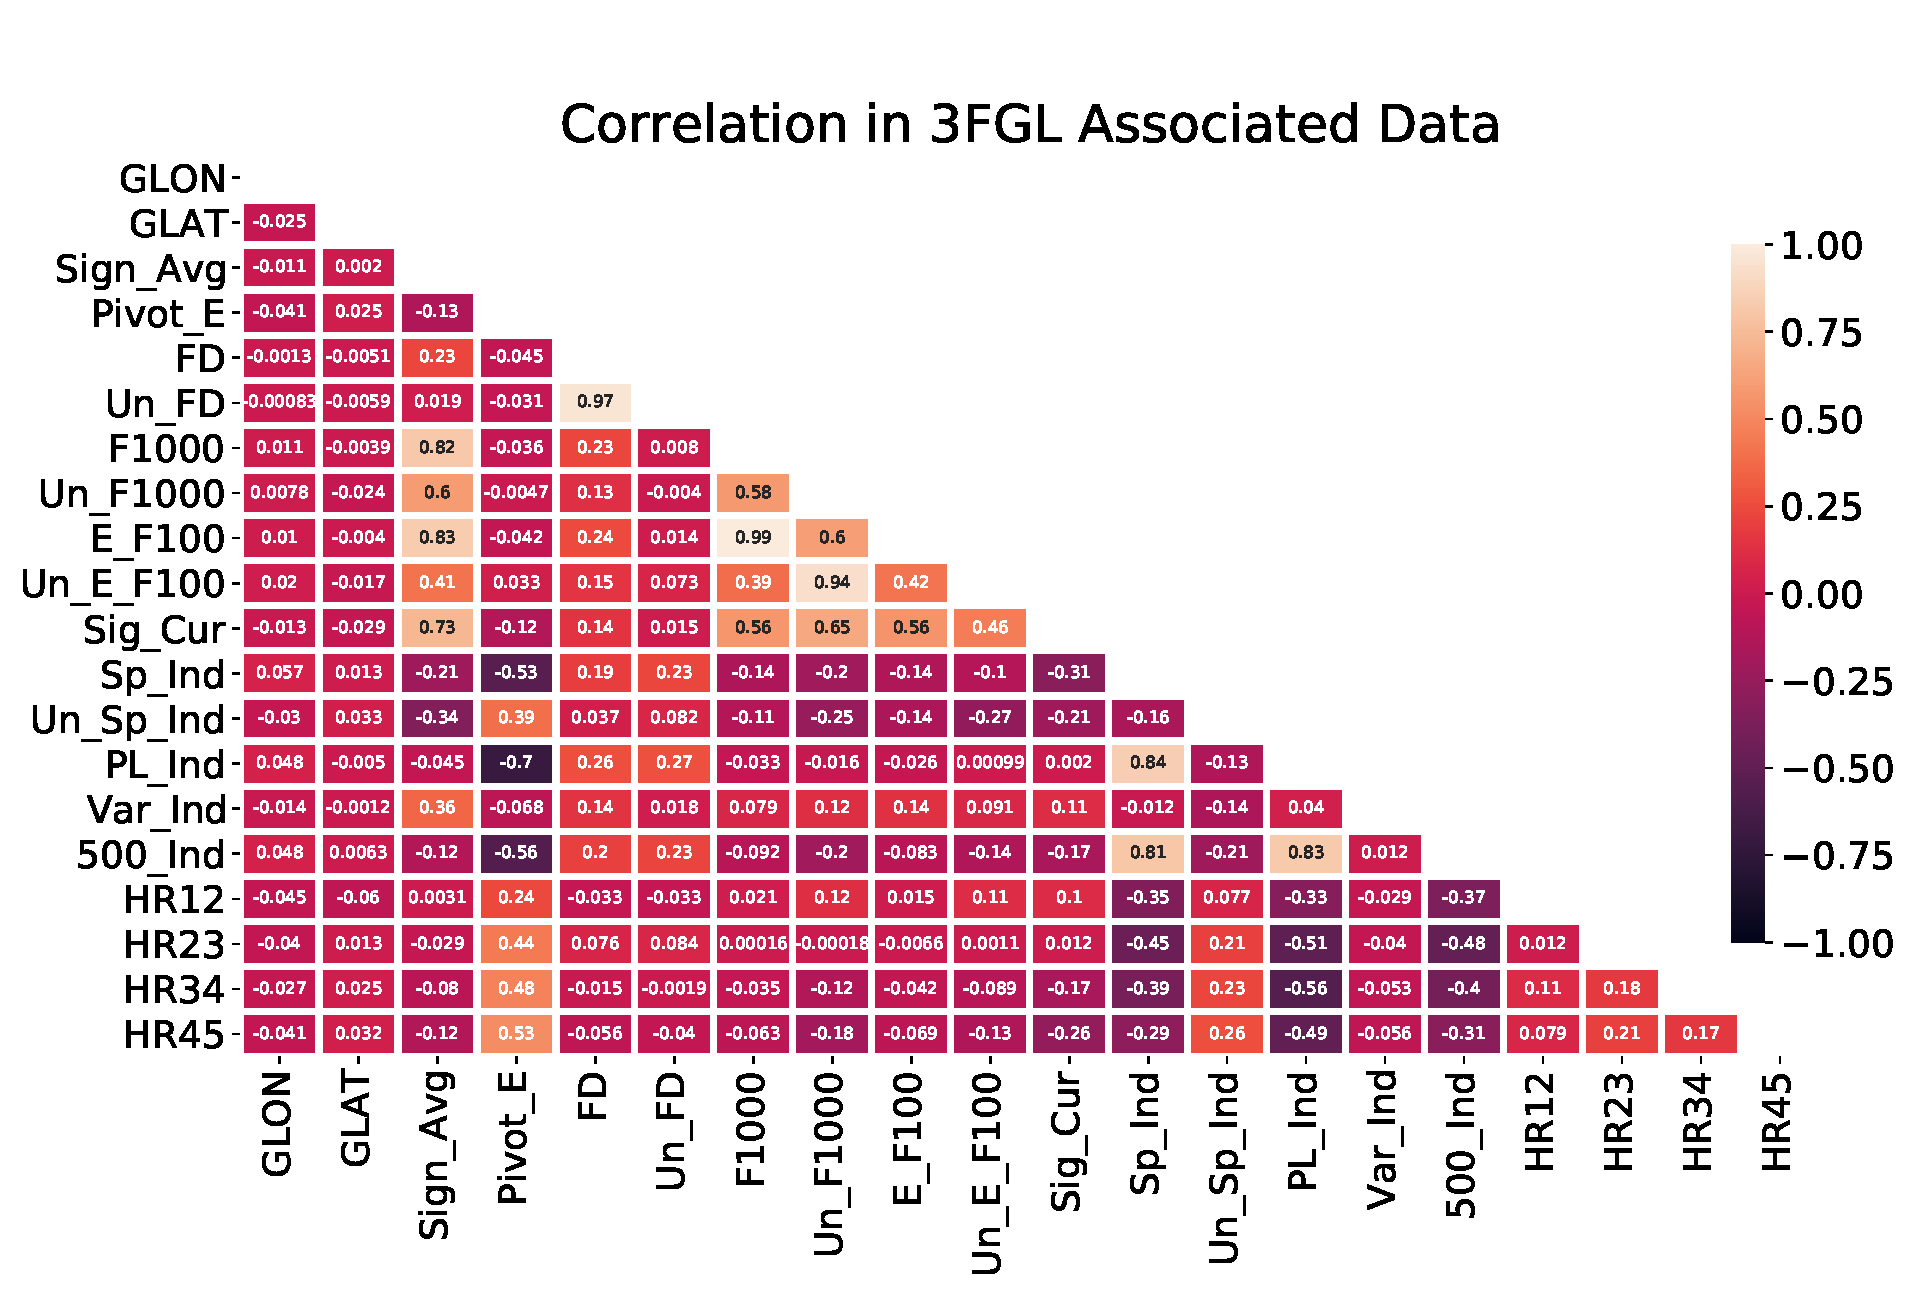
\includegraphics[width=0.5\textwidth]{plots/3fgl_assoc_cor.pdf}
\caption{The corelation matrix of features for 3FGL associated sources.
The ``500MeV\_Index'' is defined in Eq. (\ref{eq:n500_def}), all other features are taken directly 
from the 3FGL catalog.
}
\label{fig:assoc_corr_3fgli}
\end{figure}

Spectral index is one of the important characteristics of sources. 
Unfortunately in the 3FGL catalog, the definition of the spectral index is different for associated and unassociated sources.
In particular, the gamma-ray flux of pulsars is described by a power-law with a (super)exponential cutoff $\propto E^{-\Gamma} e^{-(E / E_c)^b}$ 
function, where the ``Spectral\_Index'' feature in the catalog is the parameter $\Gamma$.
Gamma-ray flux of unassociated sources with significant curvature is represented by log-parabola function $\propto (E/E_0)^{-\al - \bt \ln (E/E_0)}$,
where the ``Spectral\_Index'' feature is the parameter $\al$, i.e., the tilt in the spectrum at the pivot energy $E_0$ (which also varies for different sources).
Since the ``Spectral\_Index'' feature has different definitions for associated pulsars and for possible pulsars among unassociated sources,
its use for training the algorithms to separate pulsars from AGNs is problematic.
If one fits all spectra of sources in the catalog by a power-law function, then the corresponding indices of the power laws are represented by
``PowerLaw\_Index'' feature in the catalog.
This feature is defined uniformly for all associated and unassociated sources, i.e., it is safe to use for training.
Unfortunately, the power-law function is not a good description of the gamma-ray flux from pulsars.
Consequently, in the classification of the 3FGL sources we have constructed a new feature: the index at 500 MeV (denoted in the following as ``500MeV\_Index''), defined as minus the derivative of the log flux:
\bea
\lb{eq:n500_def}
n({\rm 500\,MeV}) = - \left. \frac{d \ln F}{d \ln E} \right|_{E = \rm 500\,MeV}
\eea
For log parabola and for power law with (super)exponential cutoff it is respectively
\bea
n(\rm 500\,MeV) &=& \al + 2 \bt \ln(\rm 500\,MeV / E_0)    \\
n({\rm 500\,MeV}) &=& \Gamma + b\,({\rm 500\,MeV} / E_c)^b
\eea
This feature has a more uniform definition for all sources in the 3FGL catalog than the Spectral\_Index. It also has a better separating power 
than PowerLaw\_Index, provided that pulsars have typically harder spectra at energies below 1 GeV than AGNs.

Taking into account the correlation among the features and the above discussion of the spectral index definition,
we have selected the following eleven features for the classification of the 3FGL sources:
Galactic latitude (GLAT), Galactic longitude (GLON), ln(Energy\_Flux\_100), $\ln$(Unc\_Energy\_Flux100), 500MeV\_Index, $\ln$(Signif\_Curve), 
$\ln$(Variability\_Index), and four hardness ratios $hr_{ij} = \frac{EF_j - EF_i}{EF_j + EF_i}$, where $EF_i$ is the energy flux in bin $i$
and $j = i + 1$ (i.e., the bins are consecutive).
We have added the hardness ratios in order to allow the algorithms to ``construct'' their own features from the raw data rather than to use the 
derived features, such as spectral index or integrated flux.
The table of features and their statistics can be found in Appendix \ref{sec:app}.






\subsection{Construction of classification algorithms}

The number of tunable parameters in the classification algorithms is not fixed a priori. 
Moreover there is a certain freedom in the choice of the architecture of the algorithms, such as
the number of hidden layers and the number of neurons in neural networks.
In general, one starts with a simple model and increases the complexity (the number of tunable parameters)
until the model can describe the data well, but does not overfit it.
The overfitting is tested by splitting the input data into the training and testing samples.
The training sample is used for optimizing the parameters,
while the test sample is used to check that the model is not overtrained (for overtrained models the accuracy on the test
sample is significantly worse than the performance on the training sample).
We will split the data randomly into 70\% training and 30\% testing samples.



\subsubsection{Random Forests}
\lb{sec:rf}

The two main parameters characterizing the RF algorithm are the number of trees and the maximum depth allowed in the trees. 
We use the Gini index as the objective function for the optimization of parameters (split values of features in the nodes).

\begin{figure}[h]
\centering
\hspace*{-0.5cm}
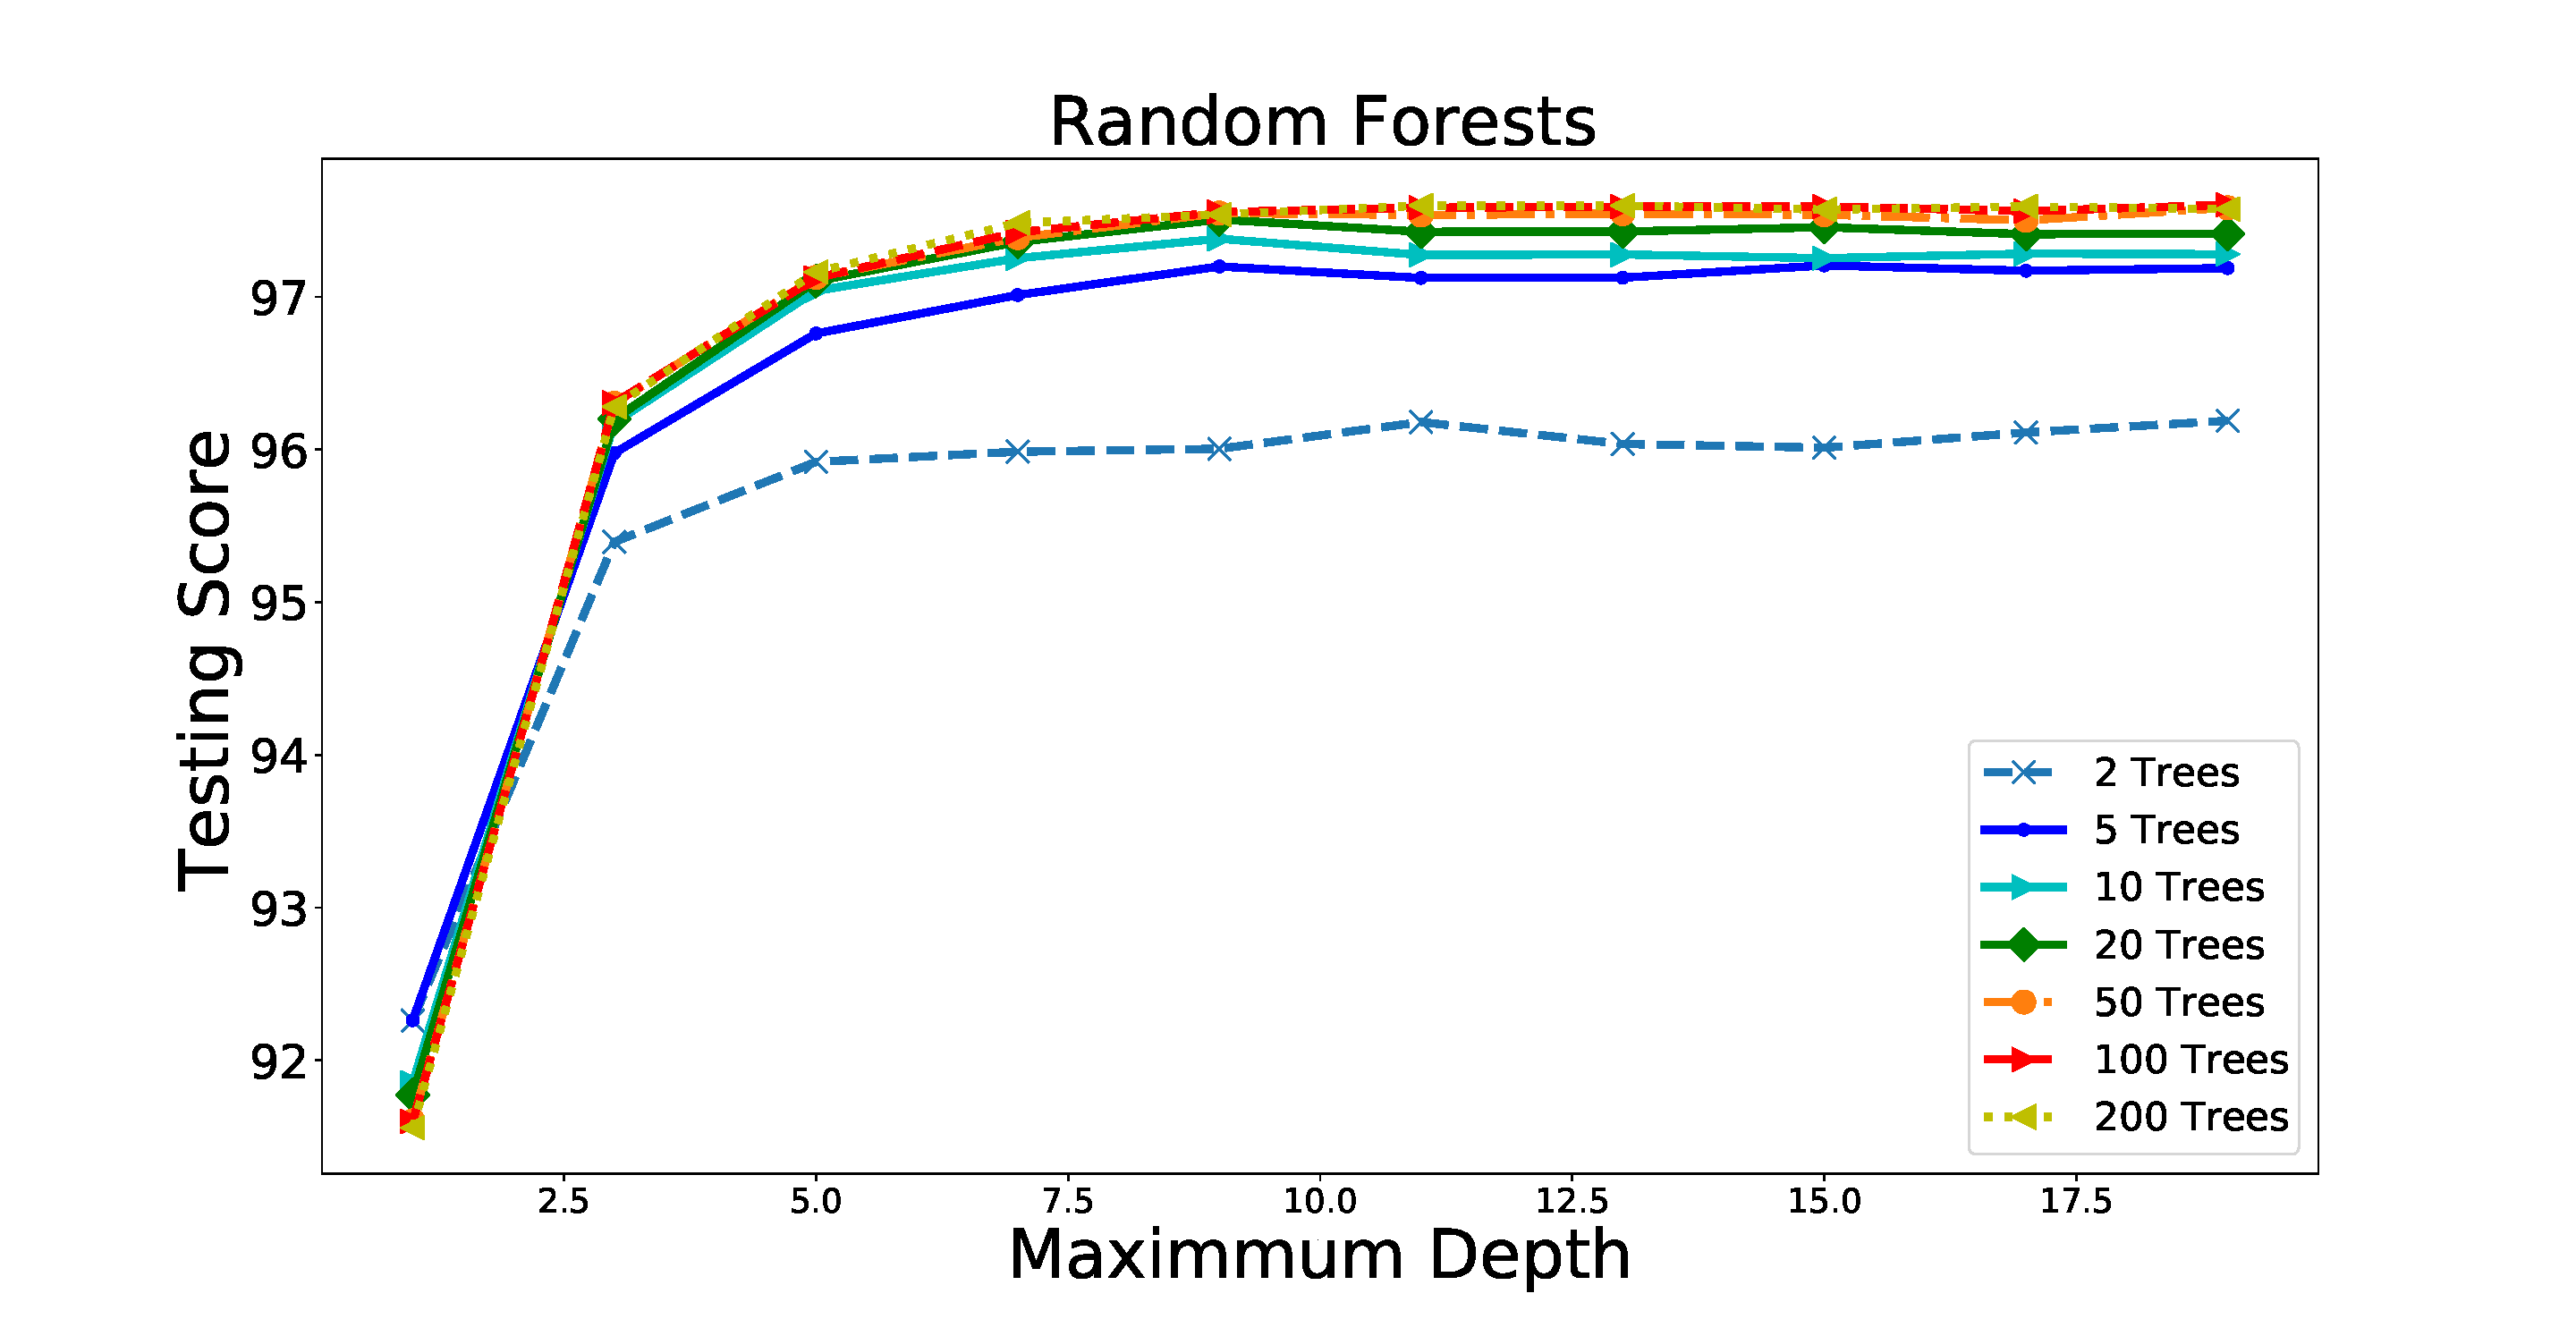
\includegraphics[width=0.5\textwidth]{plots/rf_train_assocnewfeats.pdf}
\caption{
Test score (accuracy) of RF classification as a function of the number of trees and 
the maximal depth of trees.
}
\label{fig:RF_complexity}
\end{figure}

Fig. \ref{fig:RF_complexity} shows the dependence of the accuracy of the test sample as a function of maximum depth and the number of trees. 
The results for each point are averaged over 100 realizations of the split into training and testing samples.
We notice that the accuracy does not decrease as the maximal depth of the trees increases, i.e., there is no overfitting as the complexity of the model increases with increased maximum depth.

This is due to the random choice of a subset of features at each node (maximal number of allowed features is $\sqrt{\text{\# features}}$).
It is also insensitive to the number of trees above approximately 20 trees.
For classification we will use 50 trees with the maximum depth of 6.


In order to illustrate the separation of PS into AGNs and pulsars, we retrain the RF algorithm using only two features: log of curvature significance and log of the variability index, and plot the resulting probabilities of classes in Fig. \ref{fig:RF_domains}
for the model with 50 trees with the maximum depth of 6.
The probabilities are averaged over 100 splits into training and testing samples.
It is important to note that in this plot the model is trained on only two features. Nevertheless a good testing accuracy of 97\% is reached, 
which is similar to the accuracy of the RF classification with all 11 features.
For the final classification with RF, we use 11 features and average over 1000 splits into training and testing samples.

\begin{figure}[h]
\centering
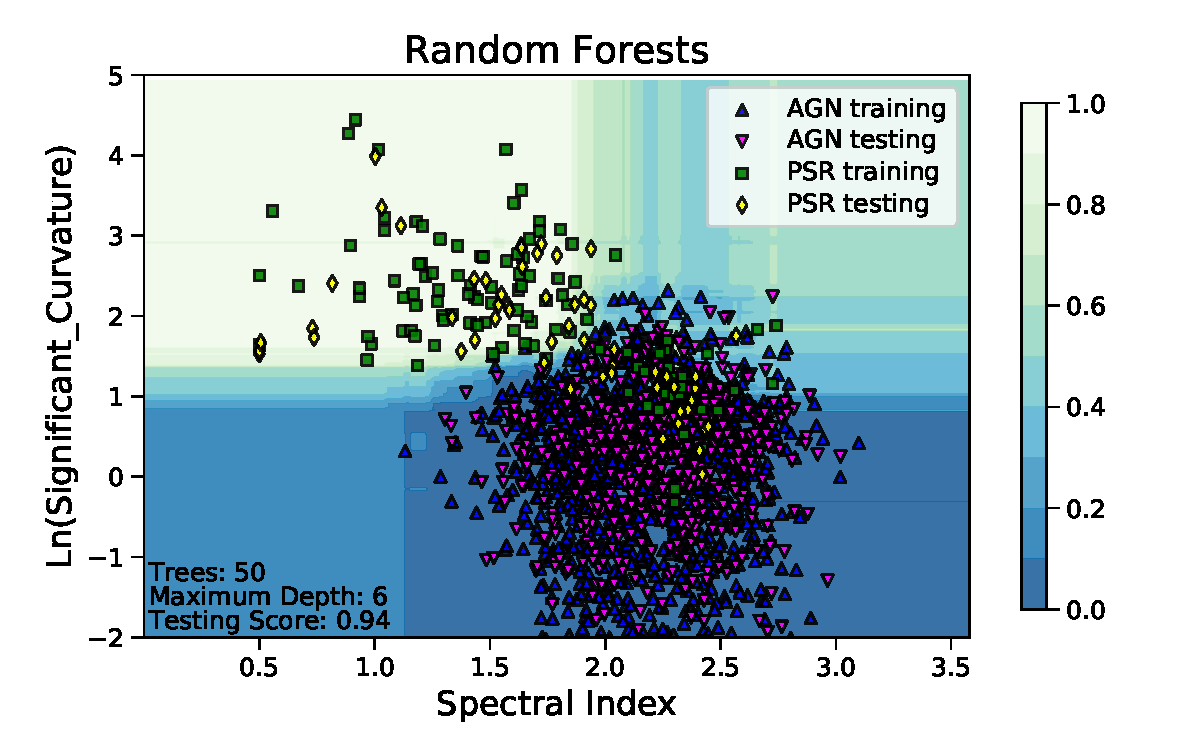
\includegraphics[width=0.5\textwidth]{plots/classification_domains/rf_50_6_final.pdf}
\caption{RF classification domains showing class probabilities for training with two features
averaged over 100 random splits into training and testing samples.
Color scale describes the probability for a source to be a pulsar.
}
\label{fig:RF_domains}
\end{figure}



\subsubsection{Boosted Decision Trees}

The meta-parameters for BDT algorithms are similar to RF algorithms: they are the number of trees and the maximal depth.
We used the Gradient Boosting algorithm for the construction of BDT \citep{gb}.
The classification is performed by a weighted average of trees, where the trees are constructed recursively in order to better address 
misclassifications from the previous step. 
Dependence of the accuracy on tree depth is shown in Fig. \ref{fig:BDT_depth}. 
Unlike the RF, which is also an ensemble based method, the testing accuracy drops for the maximal depths larger than 7. 


\begin{figure}[h]
\centering
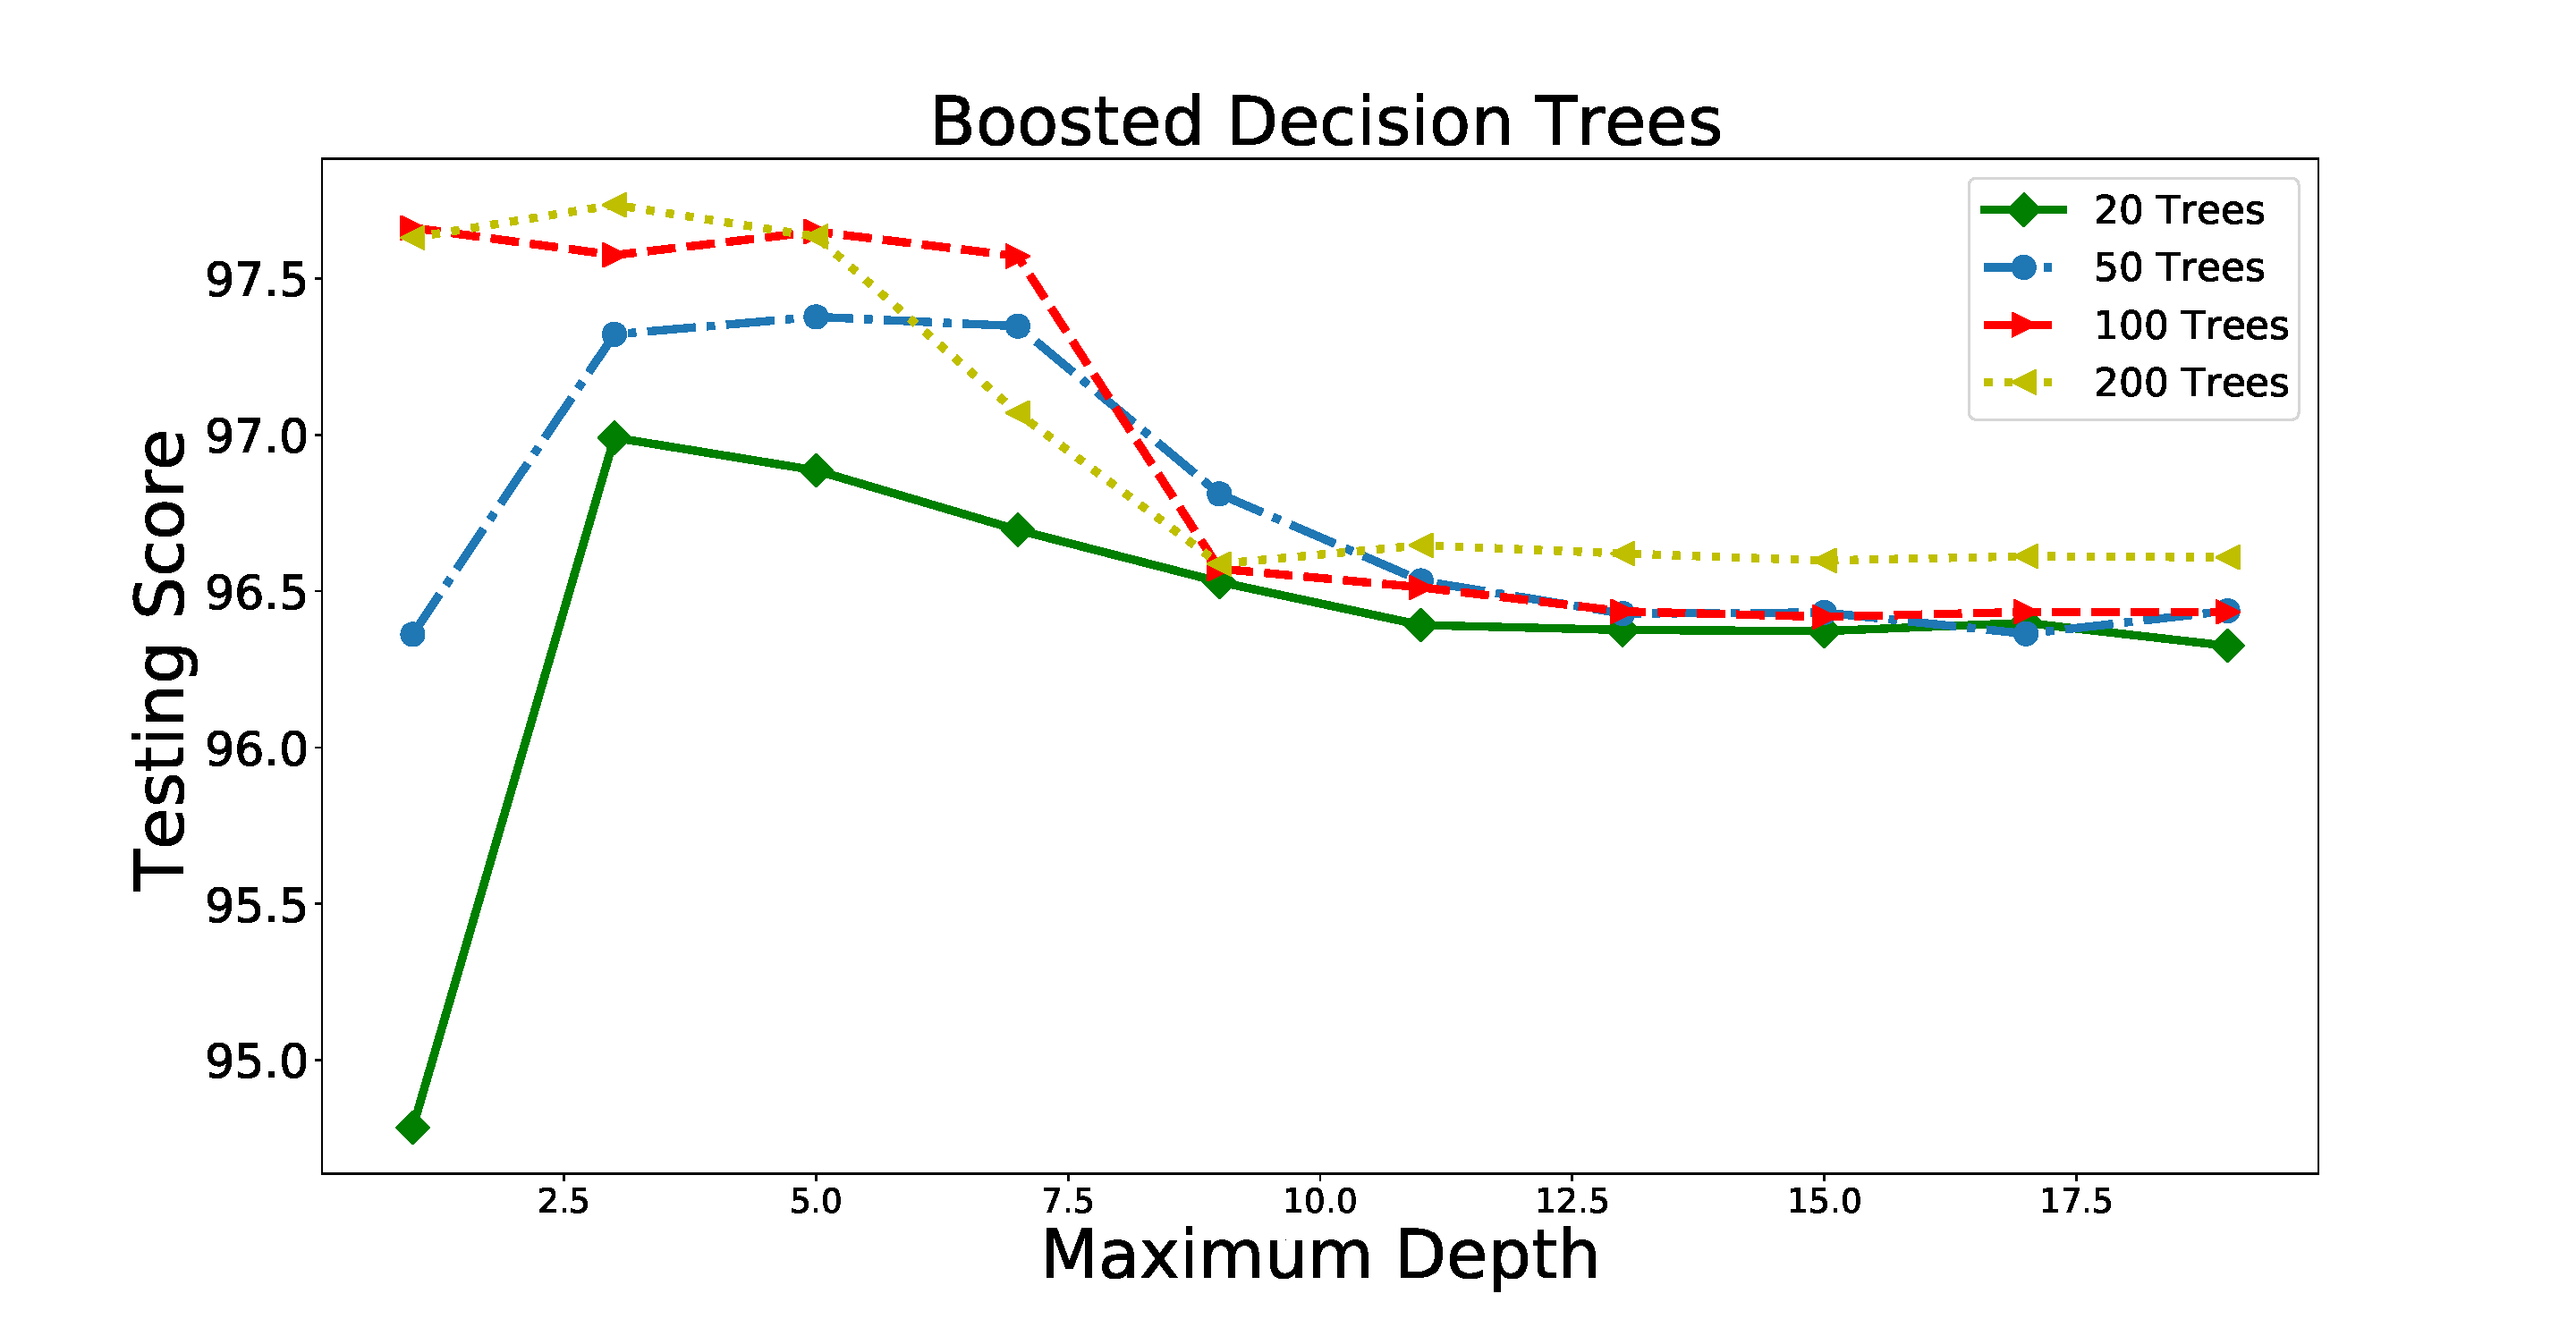
\includegraphics[width=\twopicsp\textwidth]{plots/bdt_train_assocnewfeats.pdf}
\caption{Dependence of BDT accuracy on maximum depth and the numbers of trees.}
\label{fig:BDT_depth}
\end{figure}

The classification domains in case of two features for 20 trees and the maximum depth of 2 is presented in Fig. \ref{fig:BDT_domains}. 
For the classification we will use BDT with 100 trees and the maximum depth of 2.


\begin{figure}[h]
\centering
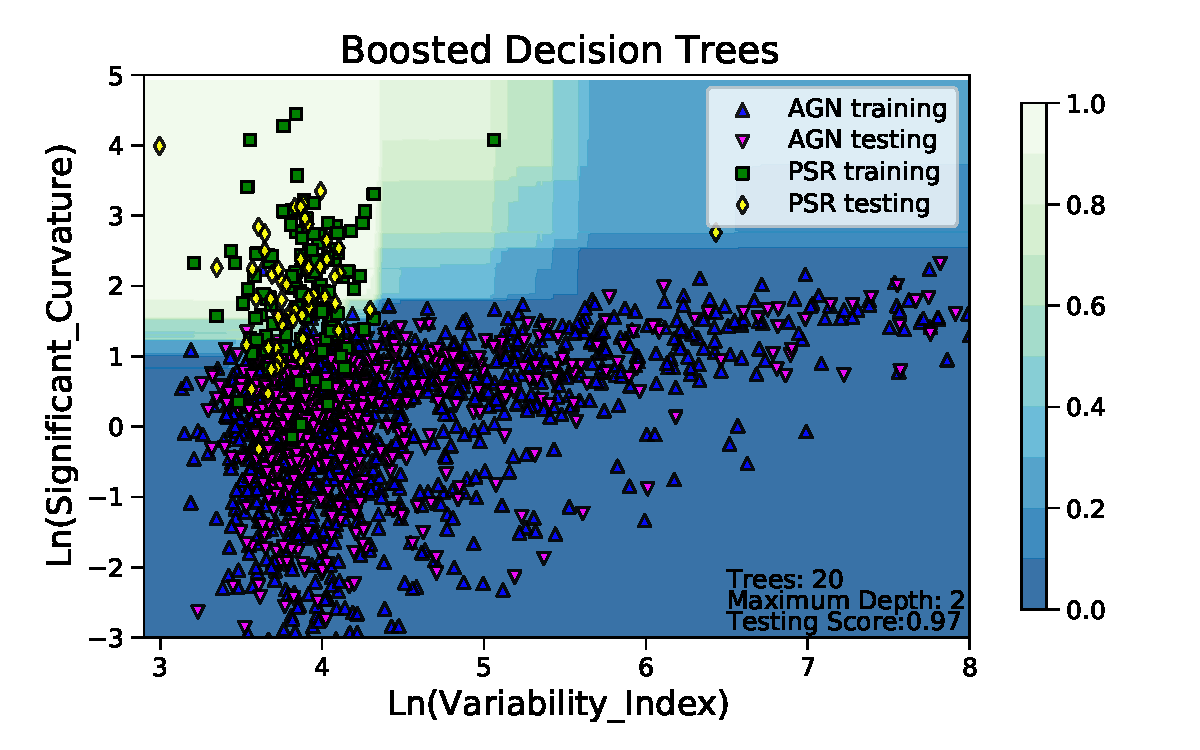
\includegraphics[width=0.5\textwidth]{plots/classification_domains/bdt_20_2.pdf}
\caption{Classification domains for BDT for training with two features 
averaged over 100 splits into training and testing samples.
}
\label{fig:BDT_domains}
\end{figure}



In tree-based algorithms, one can calculate feature importance by using the averaged reduction of impurity for nodes (Gini index in our case) involving the different features. 
The importance of features for the case of two different algorithms: RF with 50 trees and maximum depth of 6, and BDT with 100 trees with maximum depth of 2,  are shown in Table \ref{tab:feat_imp}.
We find that the most important feature for both cases is the significance of curvature.
Other significant features are the hardness ratio of the last two energy bins, uncertainty of the energy flux at 100 MeV, and the variability index.



\begin{table}[!h]
\tiny
\centering
\renewcommand{\tabcolsep}{1mm}
\renewcommand{\arraystretch}{1}

\begin{tabular}{c c c}
\hline
\hline
Feature & RF: 50, 6& BDT:100, 2\\
\hline
{ $\ln$(Signif\_Curve)}&  0.331  & 0.518   \\
{ HR45}&0.137&0.071\\
{ $\ln$(Unc\_Energy\_Flux100)} &0.122& 0.050   \\
$\ln$(Variability\_Index)& 0.098&0.225  \\
$\ln$(Energy\_Flux100) & 0.071&0.019   \\
500MeV\_Index&0.065& 0.028  \\
HR23 & 0.062&0.052  \\
HR12& 0.052&0.012  \\
HR34&0.025&0.005\\
GLAT &0.017& 0.002     \\
GLON & 0.014&0.011  \\
\hline
\end{tabular}
\vspace{0.4cm}
\caption{Feature importances for RF (50 trees, max depth 6) and BDT (100 trees, max depth 2) algorithms.
The features are ordered by decreasing importance for the RF algorithm.
}
\label{tab:feat_imp}
\end{table}

It is interesting to note that Galactic latitude is among the least significant features.
We have also used sin(GLAT) to check that this is not due to scaling, i.e., the large range of values of GLAT,
but the significance is similar to the GLAT itself.
We further discuss the dependence on GLAT in Section \ref{sec:lat-lon-profiles}, 
where we calculate the latitude and longitude profiles of the associated and unassociated source counts.
\subsubsection{Neural Networks}

In the case of NN, the number of free parameters depends on the number of hidden layers and on the number of neurons in the hidden layers. The final model accuracy also depends on the number of epochs that the network is allowed to be trained for and on the optimization algorithm. 

\begin{figure}[h]
\centering
\hspace*{-0.5cm}
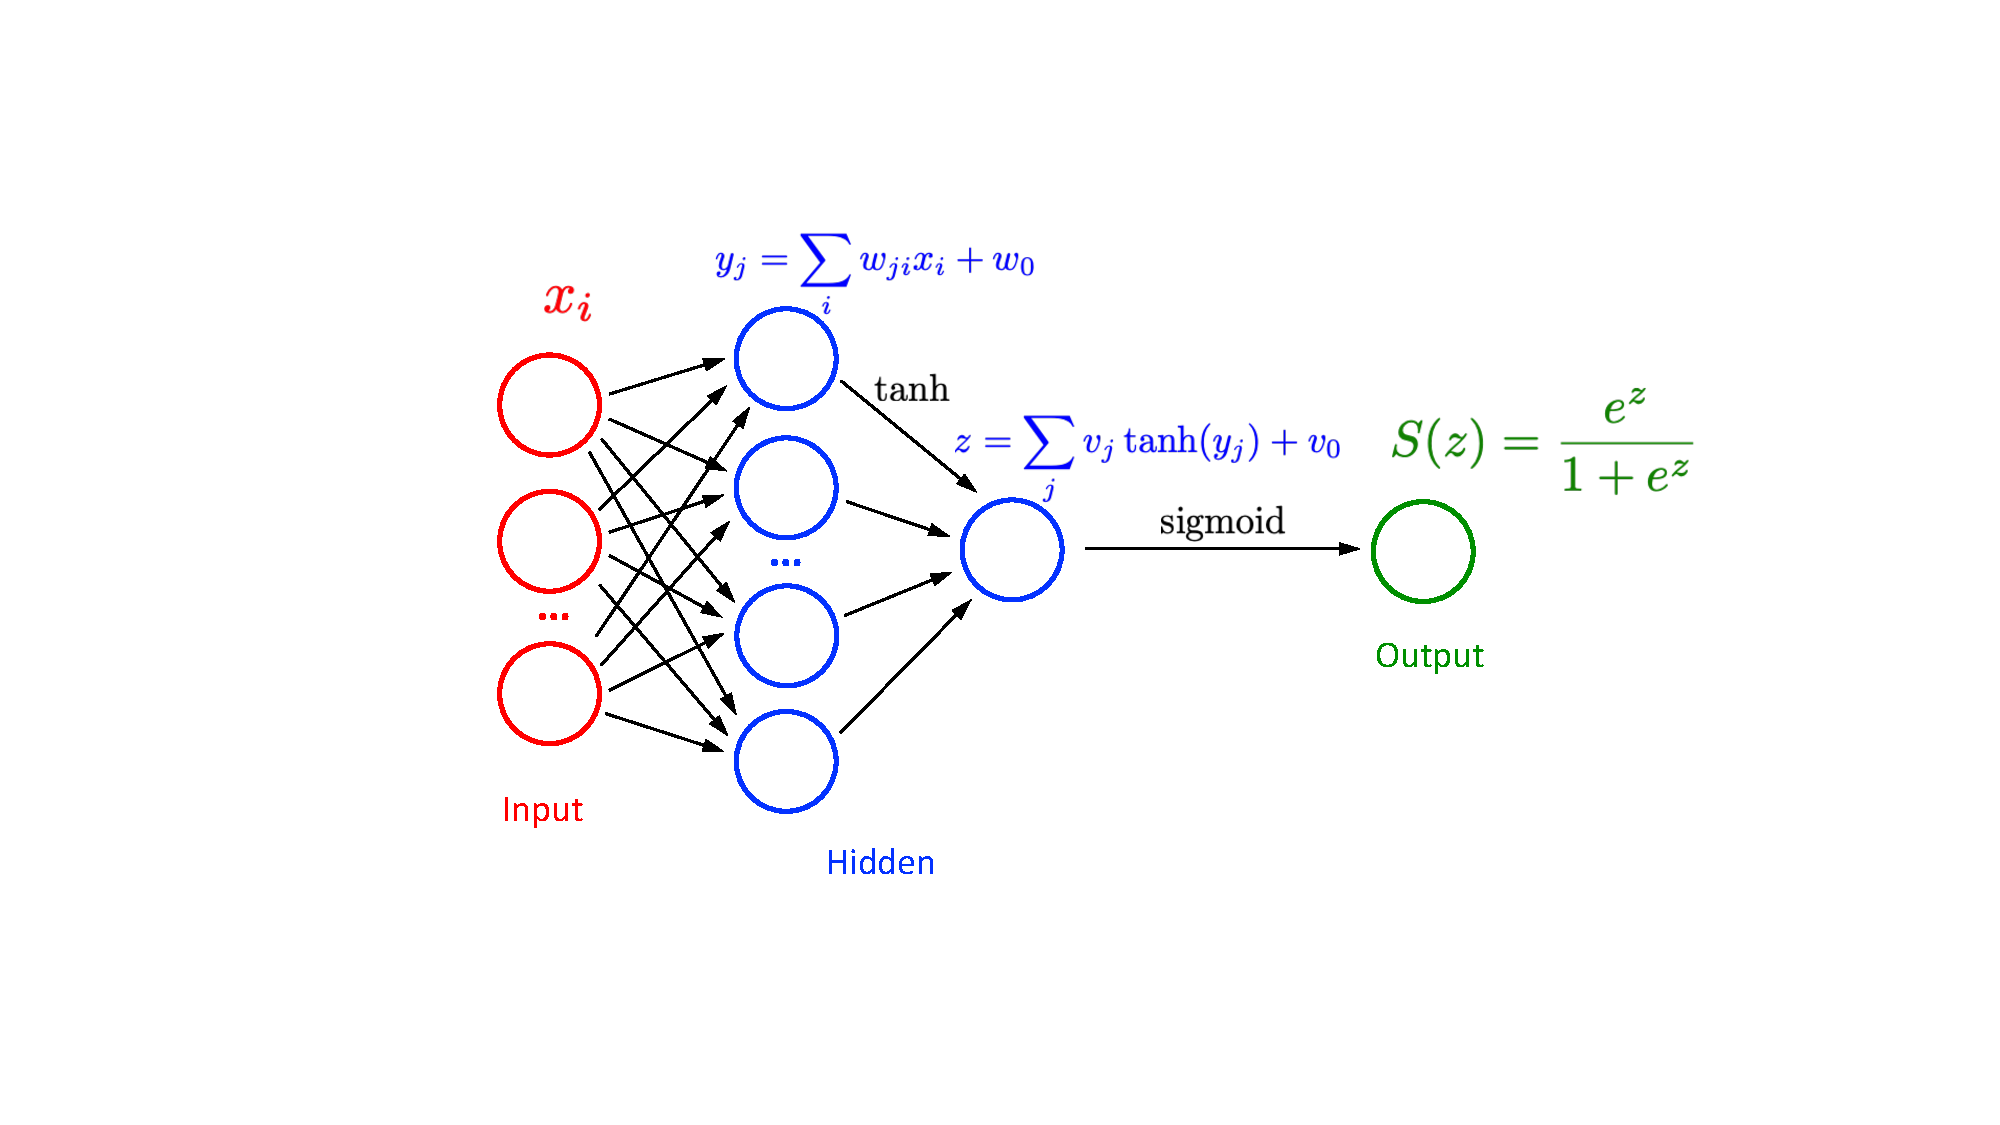
\includegraphics[width=0.45\textwidth]{plots/CNN_network.pdf}
\caption{
NN architecture that we use in the construction of the probabilistic catalogs.
The activation function in the output layer is sigmoid $S(x) = {e^{x}}/{(1 + e^{x})}$.
}
\label{fig:NN_structure}
\end{figure}

The general architecture of the NN that we use in this paper is shown in Fig. \ref{fig:NN_structure}.
It is a fully connected NN with 11 input nodes (shown by red circles with input features $x_i$), one hidden layer (shown by blue circles),
and an output layer (shown by the green circle).
The hidden layer consists of several nodes with values $y_j$. 
For the activation function at the hidden layer we use either hyperbolic tangent (tanh - shown on the plot) or rectified linear unit (relu).
The activation function for the output layer is sigmoid, which we use to make sure that the output value can be interpreted as a class probability.
The unknown parameters are weights of features in the hidden layer $w_{ji}$ and in the output layer $v_j$ including
offsets $w_{j0}$ and $v_0$.
The unknown parameters are optimized by minimizing a loss function, which we choose to be
the cross entropy
$-\text{log}L = - \sum_i (y_i\text{log}(p_i)+(1-y_i)\text{log}(1 - p_i))$, 
where $y_i = 0,\,1$ are the true labels of the sources and $p_i$ are the predicted class probabilities.
We have also used NN with two hidden layers, but the accuracy was similar to the networks with one hidden layer (Appendix \ref{sec:app}). For the final classification model, we have chosen to use one hidden layer.

\begin{figure}[h]
\centering
\hspace*{-0.5cm}
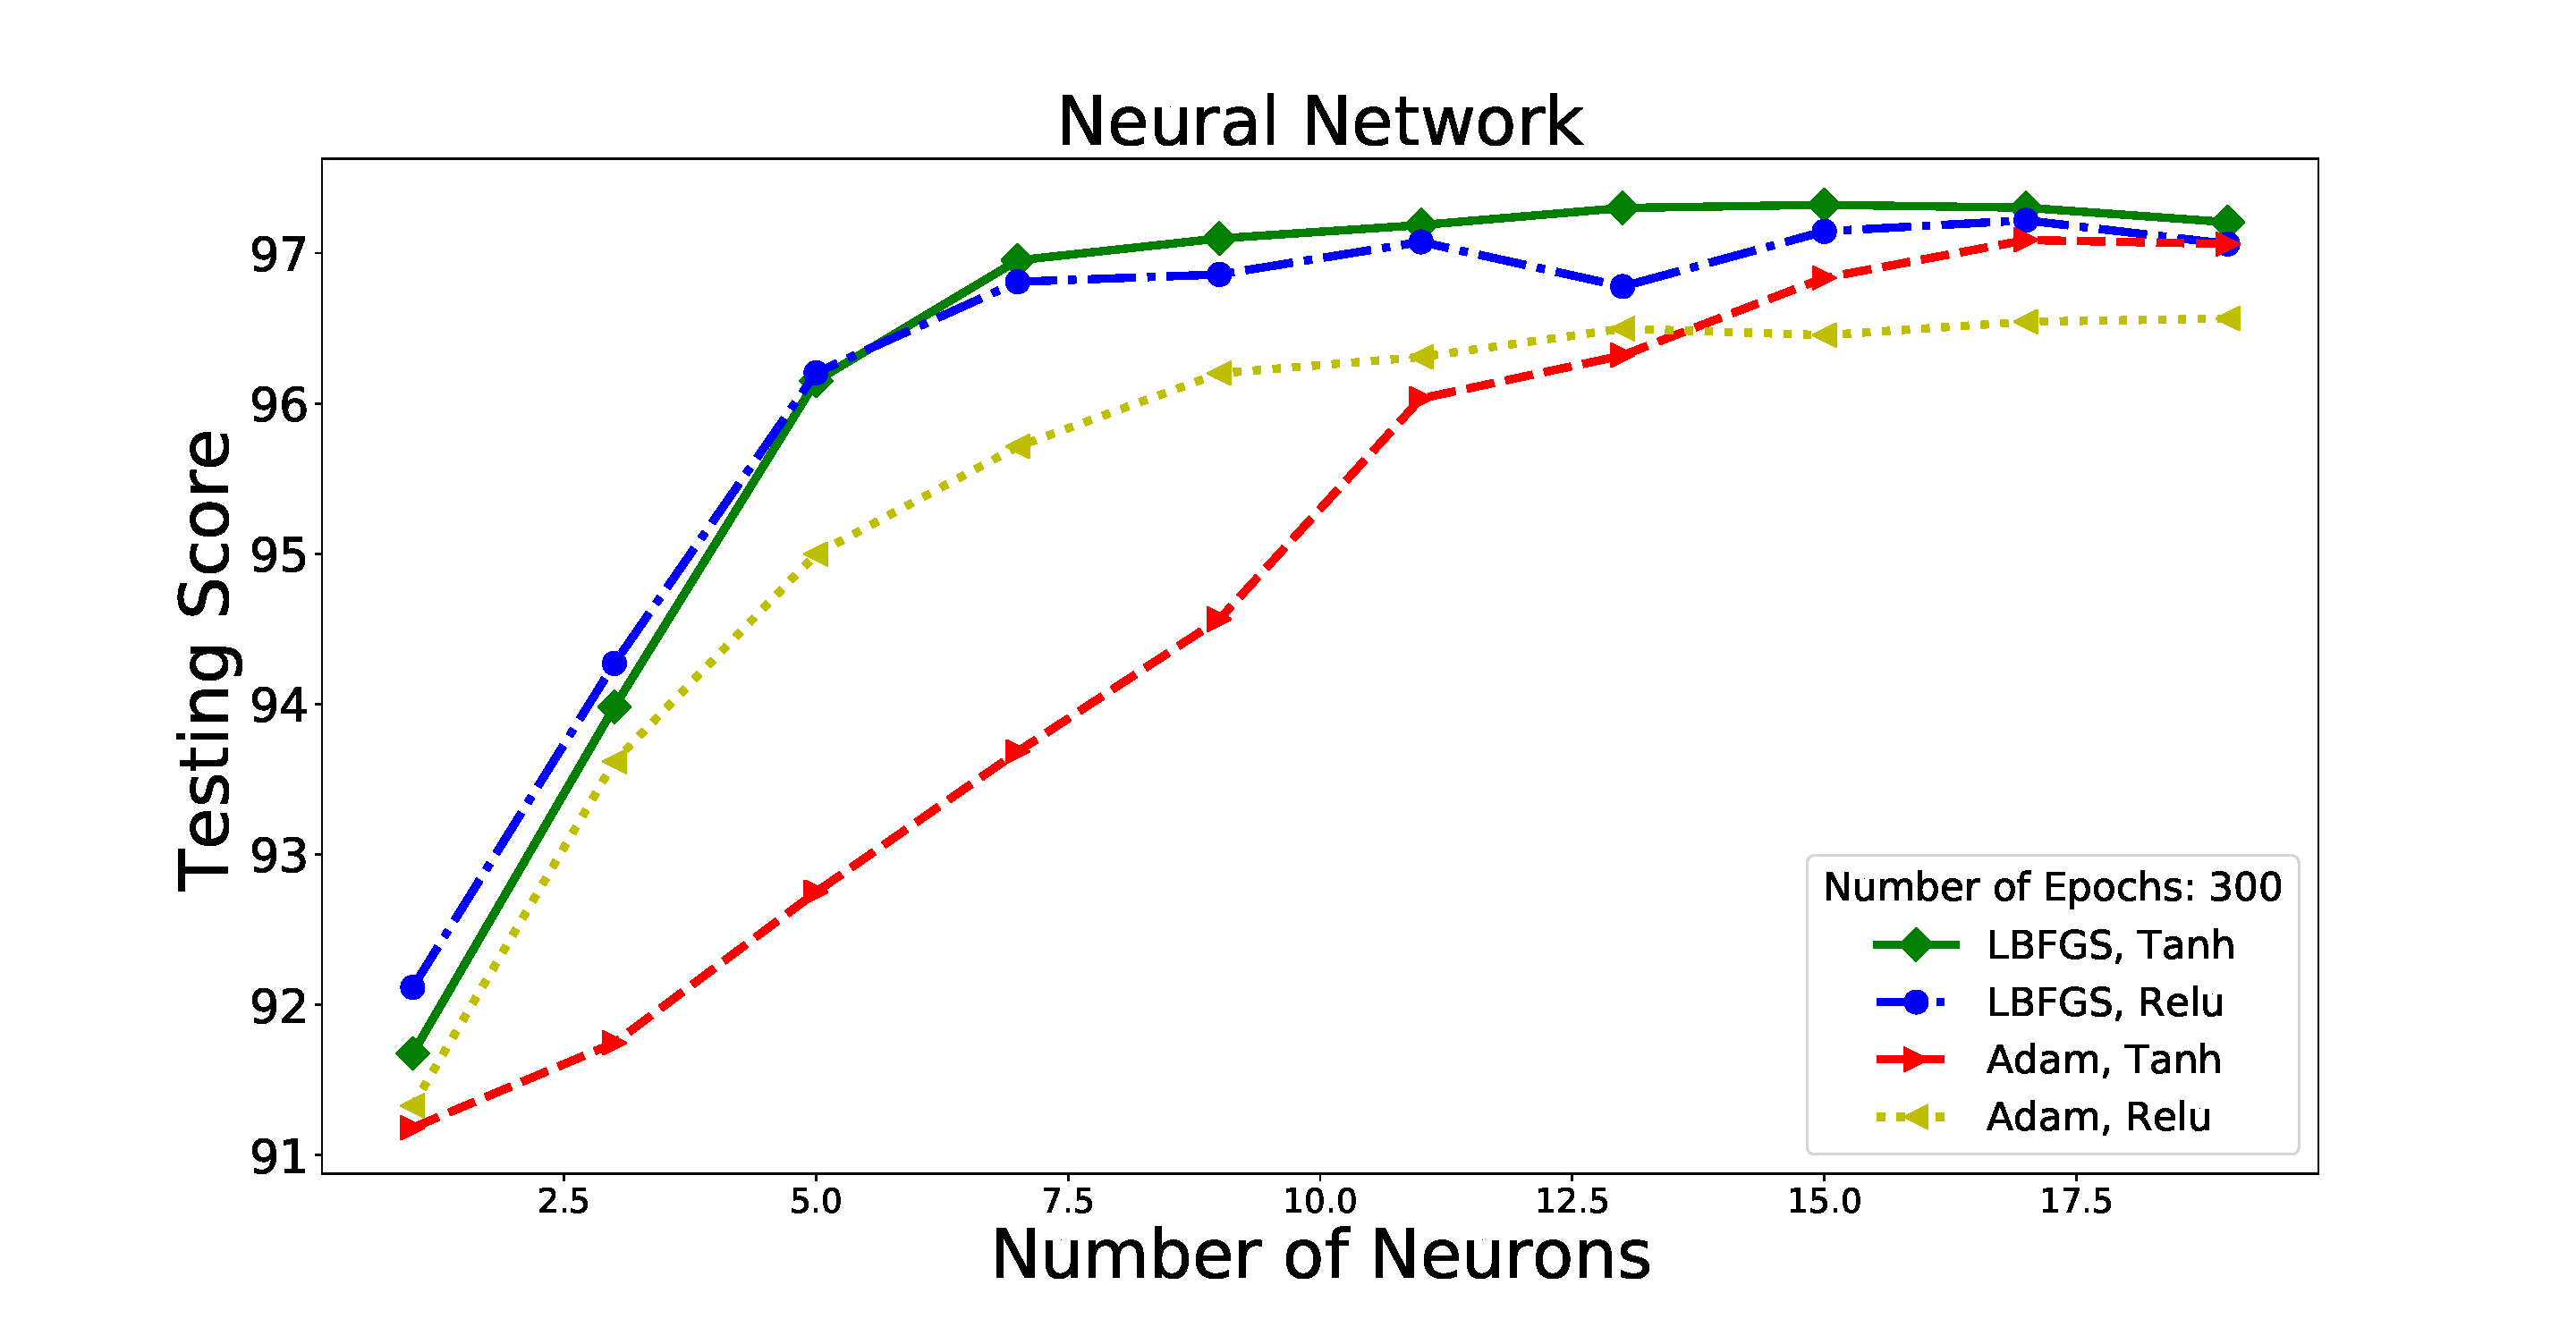
\includegraphics[width=0.5\textwidth]{plots/nn_train_neurons_assocnewfeat.pdf}
\caption{Dependence of accuracy on the number of neurons for different NN models.}
\label{fig:NN_neurons}
\end{figure}

Dependence of the testing accuracy on the number of neurons in the hidden layer, on the activation function, 
and on the optimization algorithm is shown in Fig. \ref{fig:NN_neurons}. 
We compare two activation functions at the hidden layer (tanh and relu) and two optimization algorithms: 
Limited memory Broyden-Fletcher-Goldfarb-Shanno \citep[LBFGS,][]{lbfgs} 
and the stochastic gradient descent algorithm Adam \citep{2014arXiv1412.6980K}.
We use 300 epochs for training.
Around 11 neurons in the hidden layer appears to be an optimal choice, since increasing the number of neurons leads to no significant increase in accuracy for all models. 

Dependence on the number of epochs (number of iterations in fitting) is presented in Fig. \ref{fig:NN_epochs}. 
The accuracy increases with higher number of epochs and saturates at around 200 for LBFGS and 300 for Adam. 




\begin{figure}[h]
\centering
\hspace*{-0.5cm}
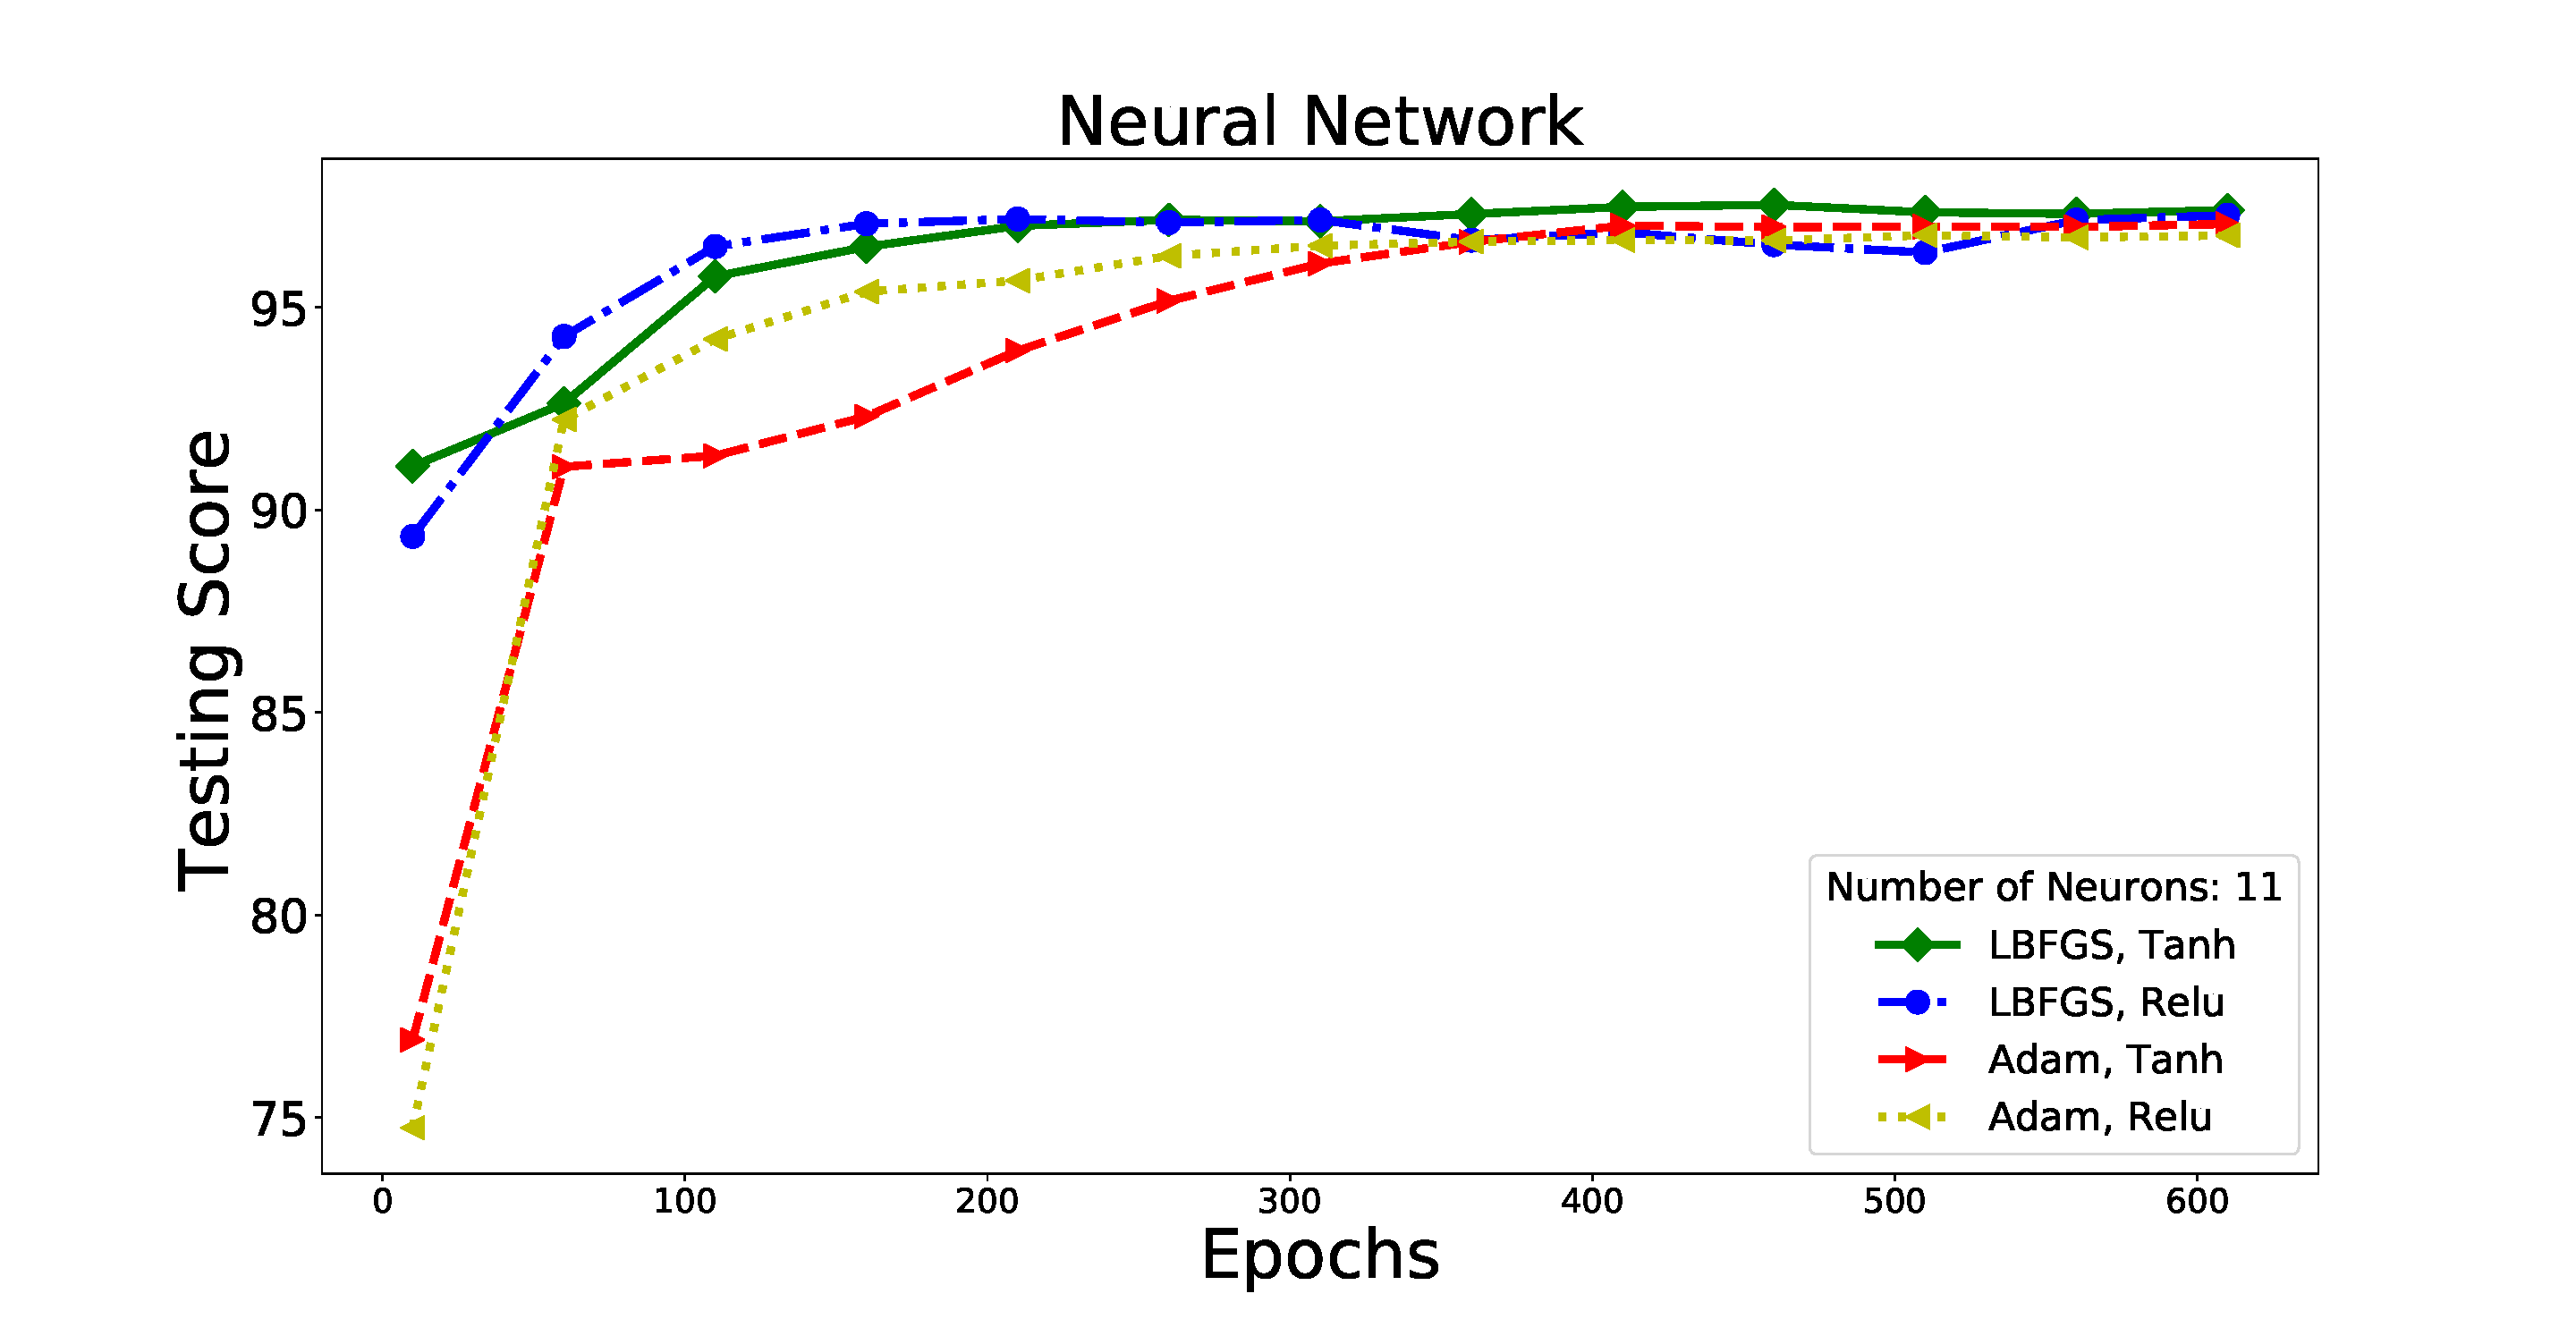
\includegraphics[width=0.5\textwidth]{plots/nn_train_epochs_assocnewfeat.pdf}
\caption{
Dependence of testing accuracy on the number of epochs in training for different solvers and activation functions.
}
\label{fig:NN_epochs}
\end{figure}
 
We illustrate the classification domains for NN with two input features in Fig. \ref{fig:NN_domains}. 
In this case we also use only two neurons in the hidden layer.
One can see that the separation boundary is smoother compared to the RF domains in Fig. \ref{fig:RF_domains} or BDT domains in Fig. \ref{fig:BDT_domains}.
For our final model we chose one hidden layer with eleven neurons, 300 training epochs, LBFGS solver, and tanh activation function at the hidden layer.


\begin{figure}[h]
\centering
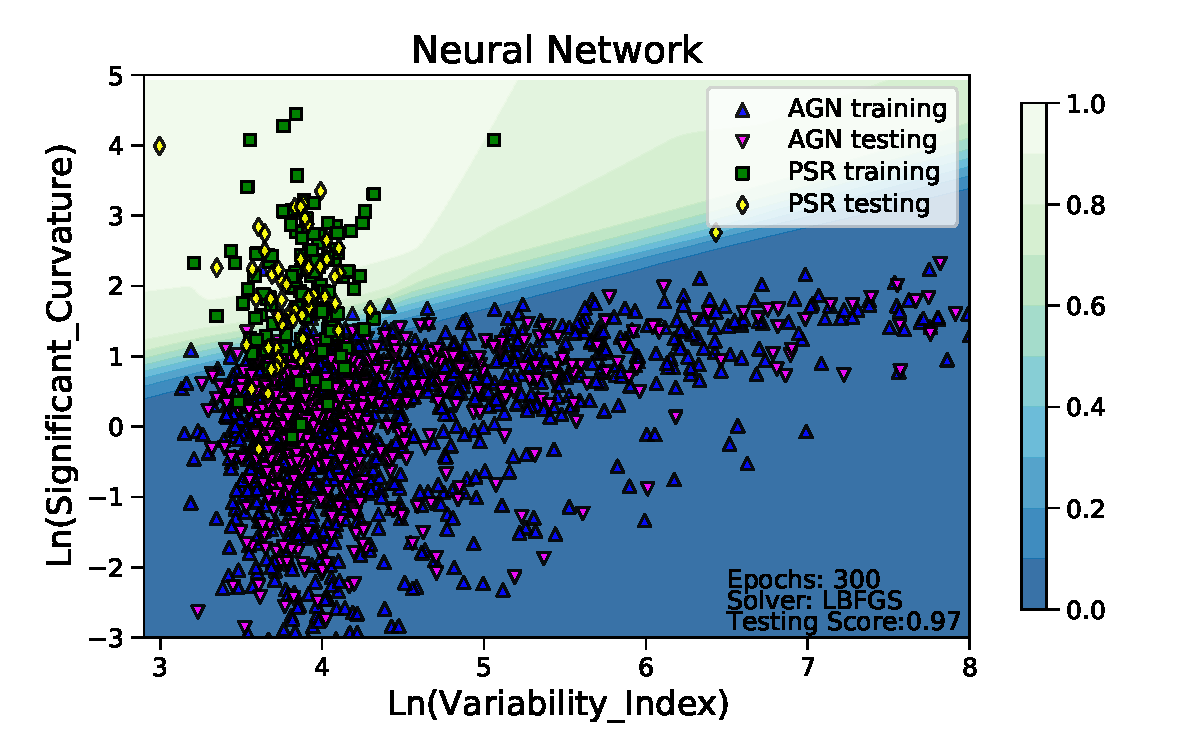
\includegraphics[width=0.5\textwidth]{plots/classification_domains/nn_300_lbfgs.pdf}
\caption{NN classification domains for 2 input features
averaged over 100 random splits into training and testing samples.
We use 2 neurons in the hidden layer. 
We use tanh activation function and LBFGS solver. 
}
\label{fig:NN_domains}
\end{figure}

\subsubsection{Logistic Regression}

As we have discussed in Section \ref{sec:class_alg}, 
the probability to belong to class 1 or 0 in LR is represented by the sigmoid function
$p_1(x) = 1 - p_0(x) = \frac{e^{m(x)}}{1 + e^{m(x)}}$ (see Eq. (\ref{eq:logit})),
where $m(x)$ is a function of input features $x$.
The complexity of the model is given by the number of parameters in $m(x)$.
We have considered two cases for $m(x)$: linear and quadratic function of the input features $x$.
Quadratic $m(x)$ resulted in a similar accuracy as linear $m(x)$.
Consequently, we have restricted our attention to linear functions $m(x) = f_0 + \sum_{k = 1}^{11} f_k x_k$.
In Fig. \ref{fig:LR_accuracy} we show the accuracy of the LR method as a function of the number of iterations
for different solvers, e.g., LBFGS \citep{lbfgs}, Stochastic Average Gradient \citep[SAG,][]{sag}, SAGA \citep[a variant of SAG,][]{saga},
and liblinear \citep[a special solver for LR and support vector machine classifications,][]{ll}.
As one can see from Fig. \ref{fig:LR_accuracy}, LBFGS and Liblinear outperform the other two solvers and converge much faster.
In order to illustrate the probability domains in LR, we show the classification with two features (LBFGs, 200 iterations)
in Fig. \ref{fig:LR_domains}. The domains look similar to the domains in the NN case (Fig. \ref{fig:NN_domains}).
For the final classification we will use LBFGs solver with 200 iterations.


\begin{figure}[h]
\centering
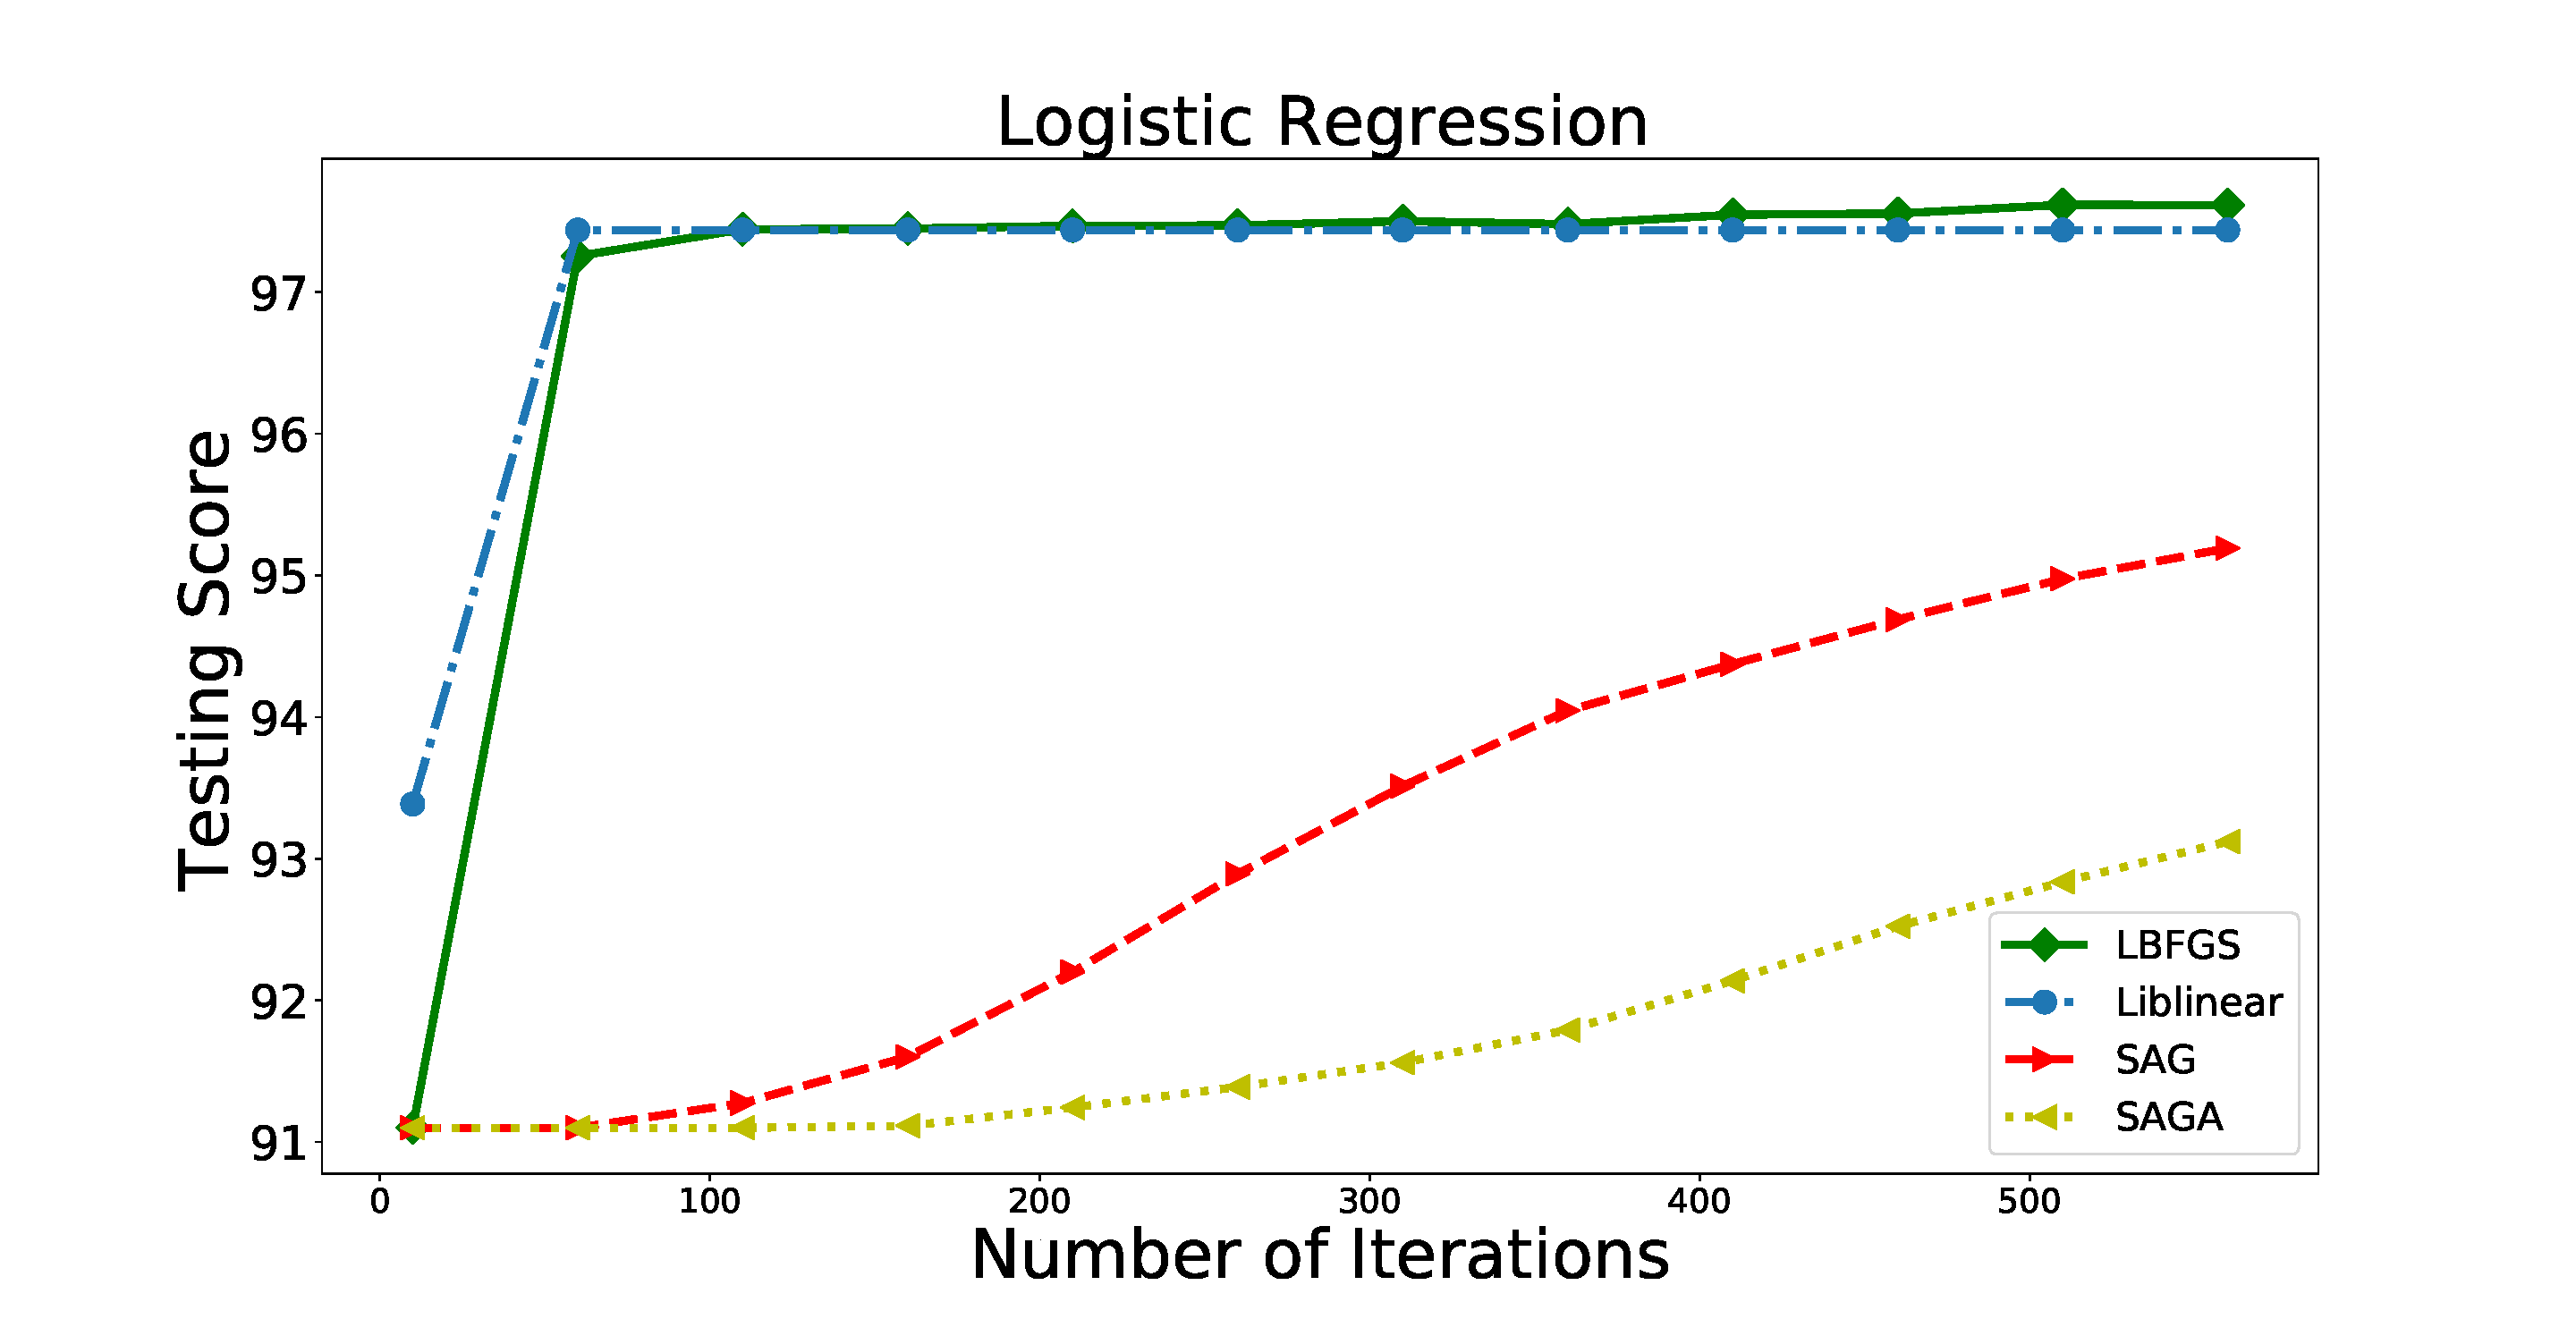
\includegraphics[width=\twopicsp\textwidth]{plots/lr_train_assocnewfeat.pdf}
\caption{Dependence of LR testing accuracy on the number of iterations for different solvers.}
\label{fig:LR_accuracy}
\end{figure}



\begin{figure}[h]
\centering
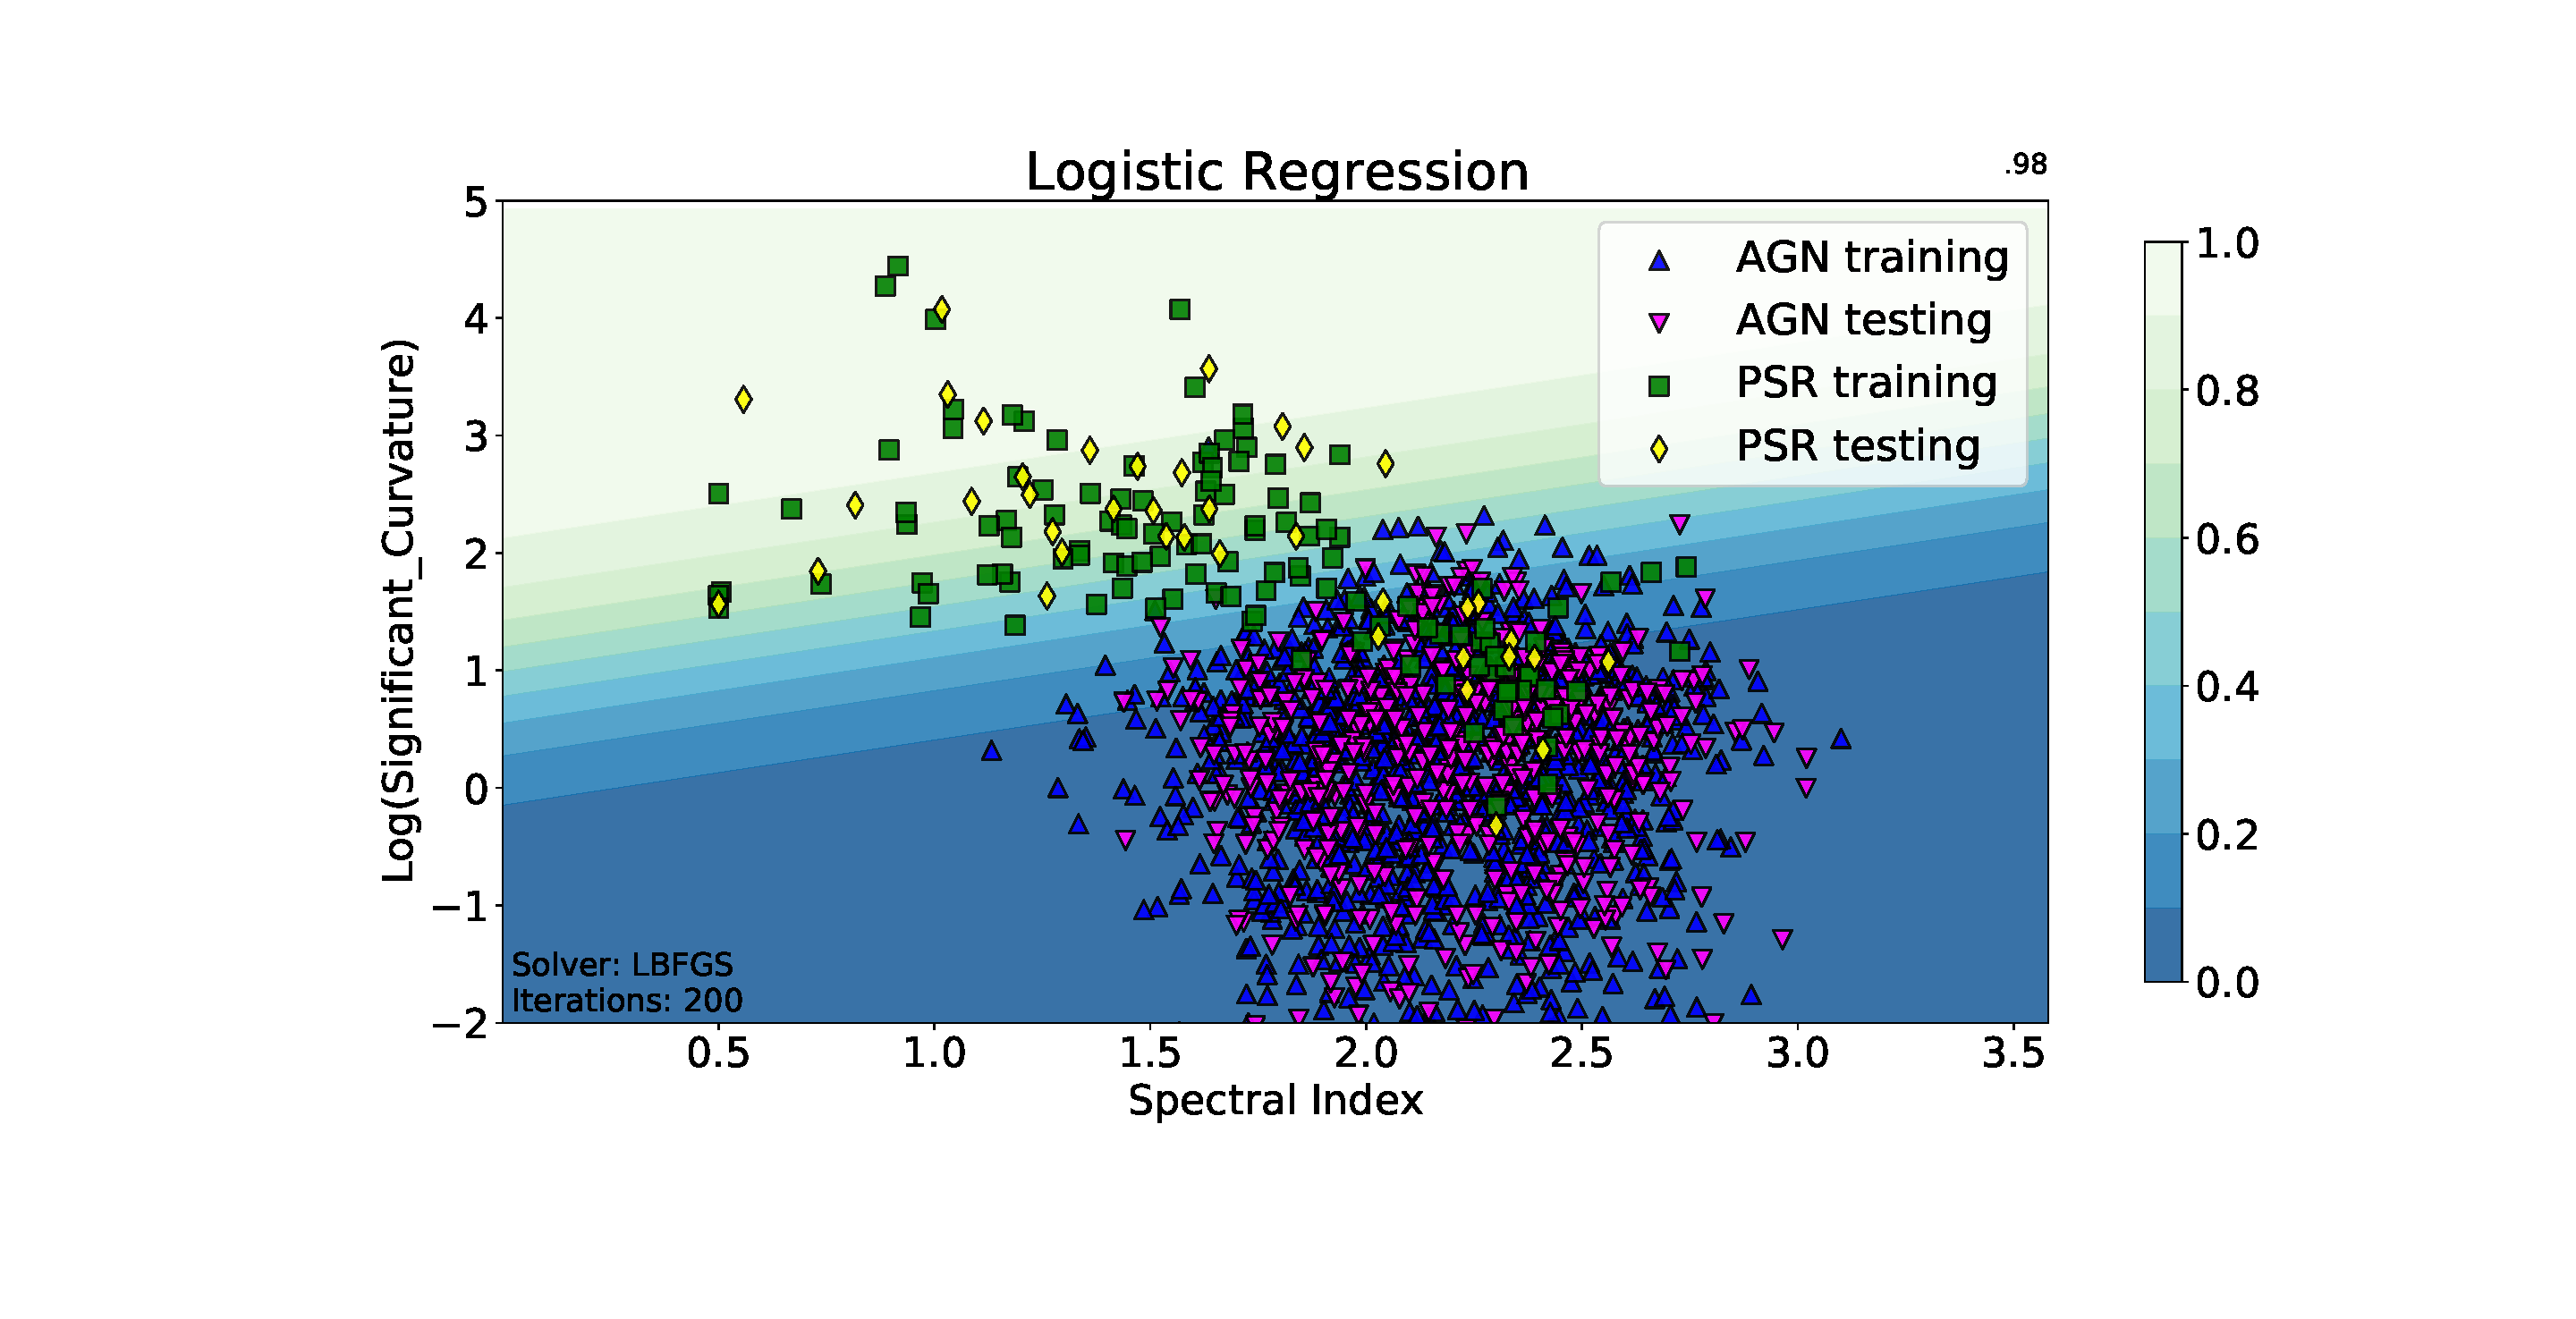
\includegraphics[width=0.5\textwidth]{plots/classification_domains/lr_200_lbfgs.pdf}
\caption{Classification domains for LR with two features 
averaged over 100 random splits into training and testing samples.}
\label{fig:LR_domains}
\end{figure}


\subsection{Oversampling}
\lb{sec:oversampling}

\Fermi-LAT catalogs have many more AGNs than pulsars, i.e., the datasets are imbalanced.
For example, the 3FGL catalog has 1744 associated AGNs and 167 associated pulsars.
In the previous subsections we have optimized the overall accuracy. In this case, the algorithms try to identify AGNs rather than pulsars,
since it gives better accuracy. As a result, in the region of parameter space, where both pulsars and AGNs are present, the algorithms
will give higher probability for a source to be an AGN.


The problem of classification of imbalanced datasets can be quantitatively described in terms of precision and recall.
If we denote by ``\# true'' the number of pulsars in the dataset, by ``\# positive'' -- the number of sources predicted to be pulsars, and by 
``\# true positive'' -- the number of pulsars predicted to be pulsars, then  $precision \rm = \frac{\#\ true\ positive}{\#\ positive}$ is a measure how clean the prediction is, while $recall \rm = \frac{\#\ true\ positive}{\#\ true}$ is a measure how well the algorithm can detect the pulsars, i.e., how complete is the list of predicted pulsars.
If we reduce the pulsar domain by attributing uncertain sources predominantly to AGNs, then for pulsars the precision will increase, but the recall will decrease.



\begin{figure}[h]
\centering
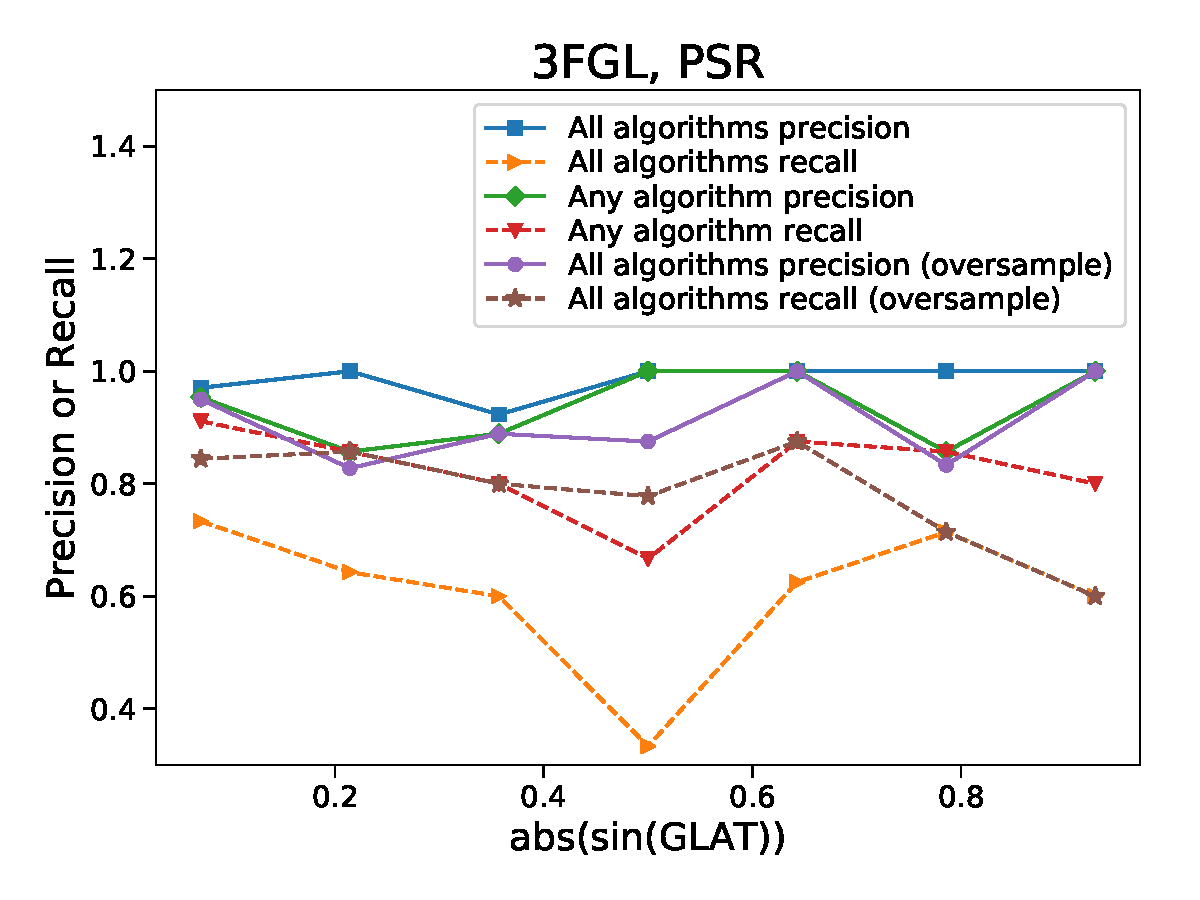
\includegraphics[width=\twopicsp\textwidth]{plots/all_algs_3FGL_precision_recall_oversample_PSR.pdf}
\caption{Precision and recall for pulsars using all-algorithm and any-algorithm classification for unweighted training data and
all-algorithm classification for oversampling of pulsars in training data. For details see Section \ref{sec:oversampling}.}
\label{fig:prec_recall}
\end{figure}


In Fig. \ref{fig:prec_recall} we show precision and recall for classification of pulsars.
In particular, in the first two lines (solid blue with squares and dashed orange with right triangles) a source is categorized as a pulsar if all four algorithms classify it as a pulsar,
while in lines 3 and 4 (solid green with diamonds and dashed red with down triangles) a source is attributed to the PSR class, if any of the algorithms classifies it as a pulsar.
It is clear that for lines 1 and 2 the pulsar domain is smaller than for lines 3 and 4, since in the former case, the domain is the intersection of domains for individual algorithms, while in the latter it is the union.
For all-algorithms classification the precision is 100\% for most of latitudes, while the recall is between 40\% and 80\%, i.e., the list of pulsars is generally clean but incomplete.
In case of any-algorithm classification, the recall is increased by about 20\% for most latitudes compared to the all-algorithms classification, but the precision drops by up to 20\% at some latitudes, i.e., the completeness improves at the expense of cleanliness of the sample.
Alternatively to using any-algorithm classification, one can give larger weights to pulsars or oversample pulsars in the training process, i.e., use the same source several times, so that the numbers of pulsars and AGNs in training are the same.
Provided that in some applications it is beneficial to have as complete as possible the list of pulsar candidates among unassociated sources, we have retrained the algorithms using oversampling with the same meta-parameters as in the previous sections.

In general one can either under- or oversample a dataset. Undersampling would reduce the number of AGNs to match the number of pulsars. However, since the total number of sources is not very high, we have chosen oversampling. 
For training with oversampling, we copy randomly existing pulsars and add them to the dataset until the number of pulsars and AGNs are the same.
Although pulsars in the training dataset are redundant, they help to increase the weight of pulsars in the classification model.
We illustrate the oversampling procedure in Fig. \ref{fig:LR_domains_O} top panel:
the number of times a source appears in training is shown by adding markers with shifts to the right and above the original position of the source (note that the shift is introduced for presentation only, the parameters of the sources are exactly the same as in the original source).
In the bottom panel of Fig. \ref{fig:LR_domains_O} we repeat Fig.  \ref{fig:LR_domains} in order to compare the classification domains with and without oversampling.
One can see that pulsar domain in the top panel is larger than the pulsar domain in the bottom panel.
As a result, in the top panel more pulsars are classified as pulsars but also more AGNs are falsely classified as pulsars in the intersection region. 
Since the overall number of AGNs is larger than the number of pulsars, the testing accuracy with oversampling is smaller than without oversampling.

The results of training with oversampling are presented  in Fig. \ref{fig:prec_recall},
lines 5 and 6 (solid purple with circles and dashed brown with stars). 
These lines show precision and recall when a source is categorized as a pulsar, if all four algorithms trained with oversampling classify it as a pulsar. 
The precision and recall in this case are similar to the any-algorithm classification for the training without oversampling.


\begin{figure}[h]
\centering

\includegraphics[width=0.5\textwidth]{plots/classification_domains/lr_200_lbfgs_oversample.pdf} \\
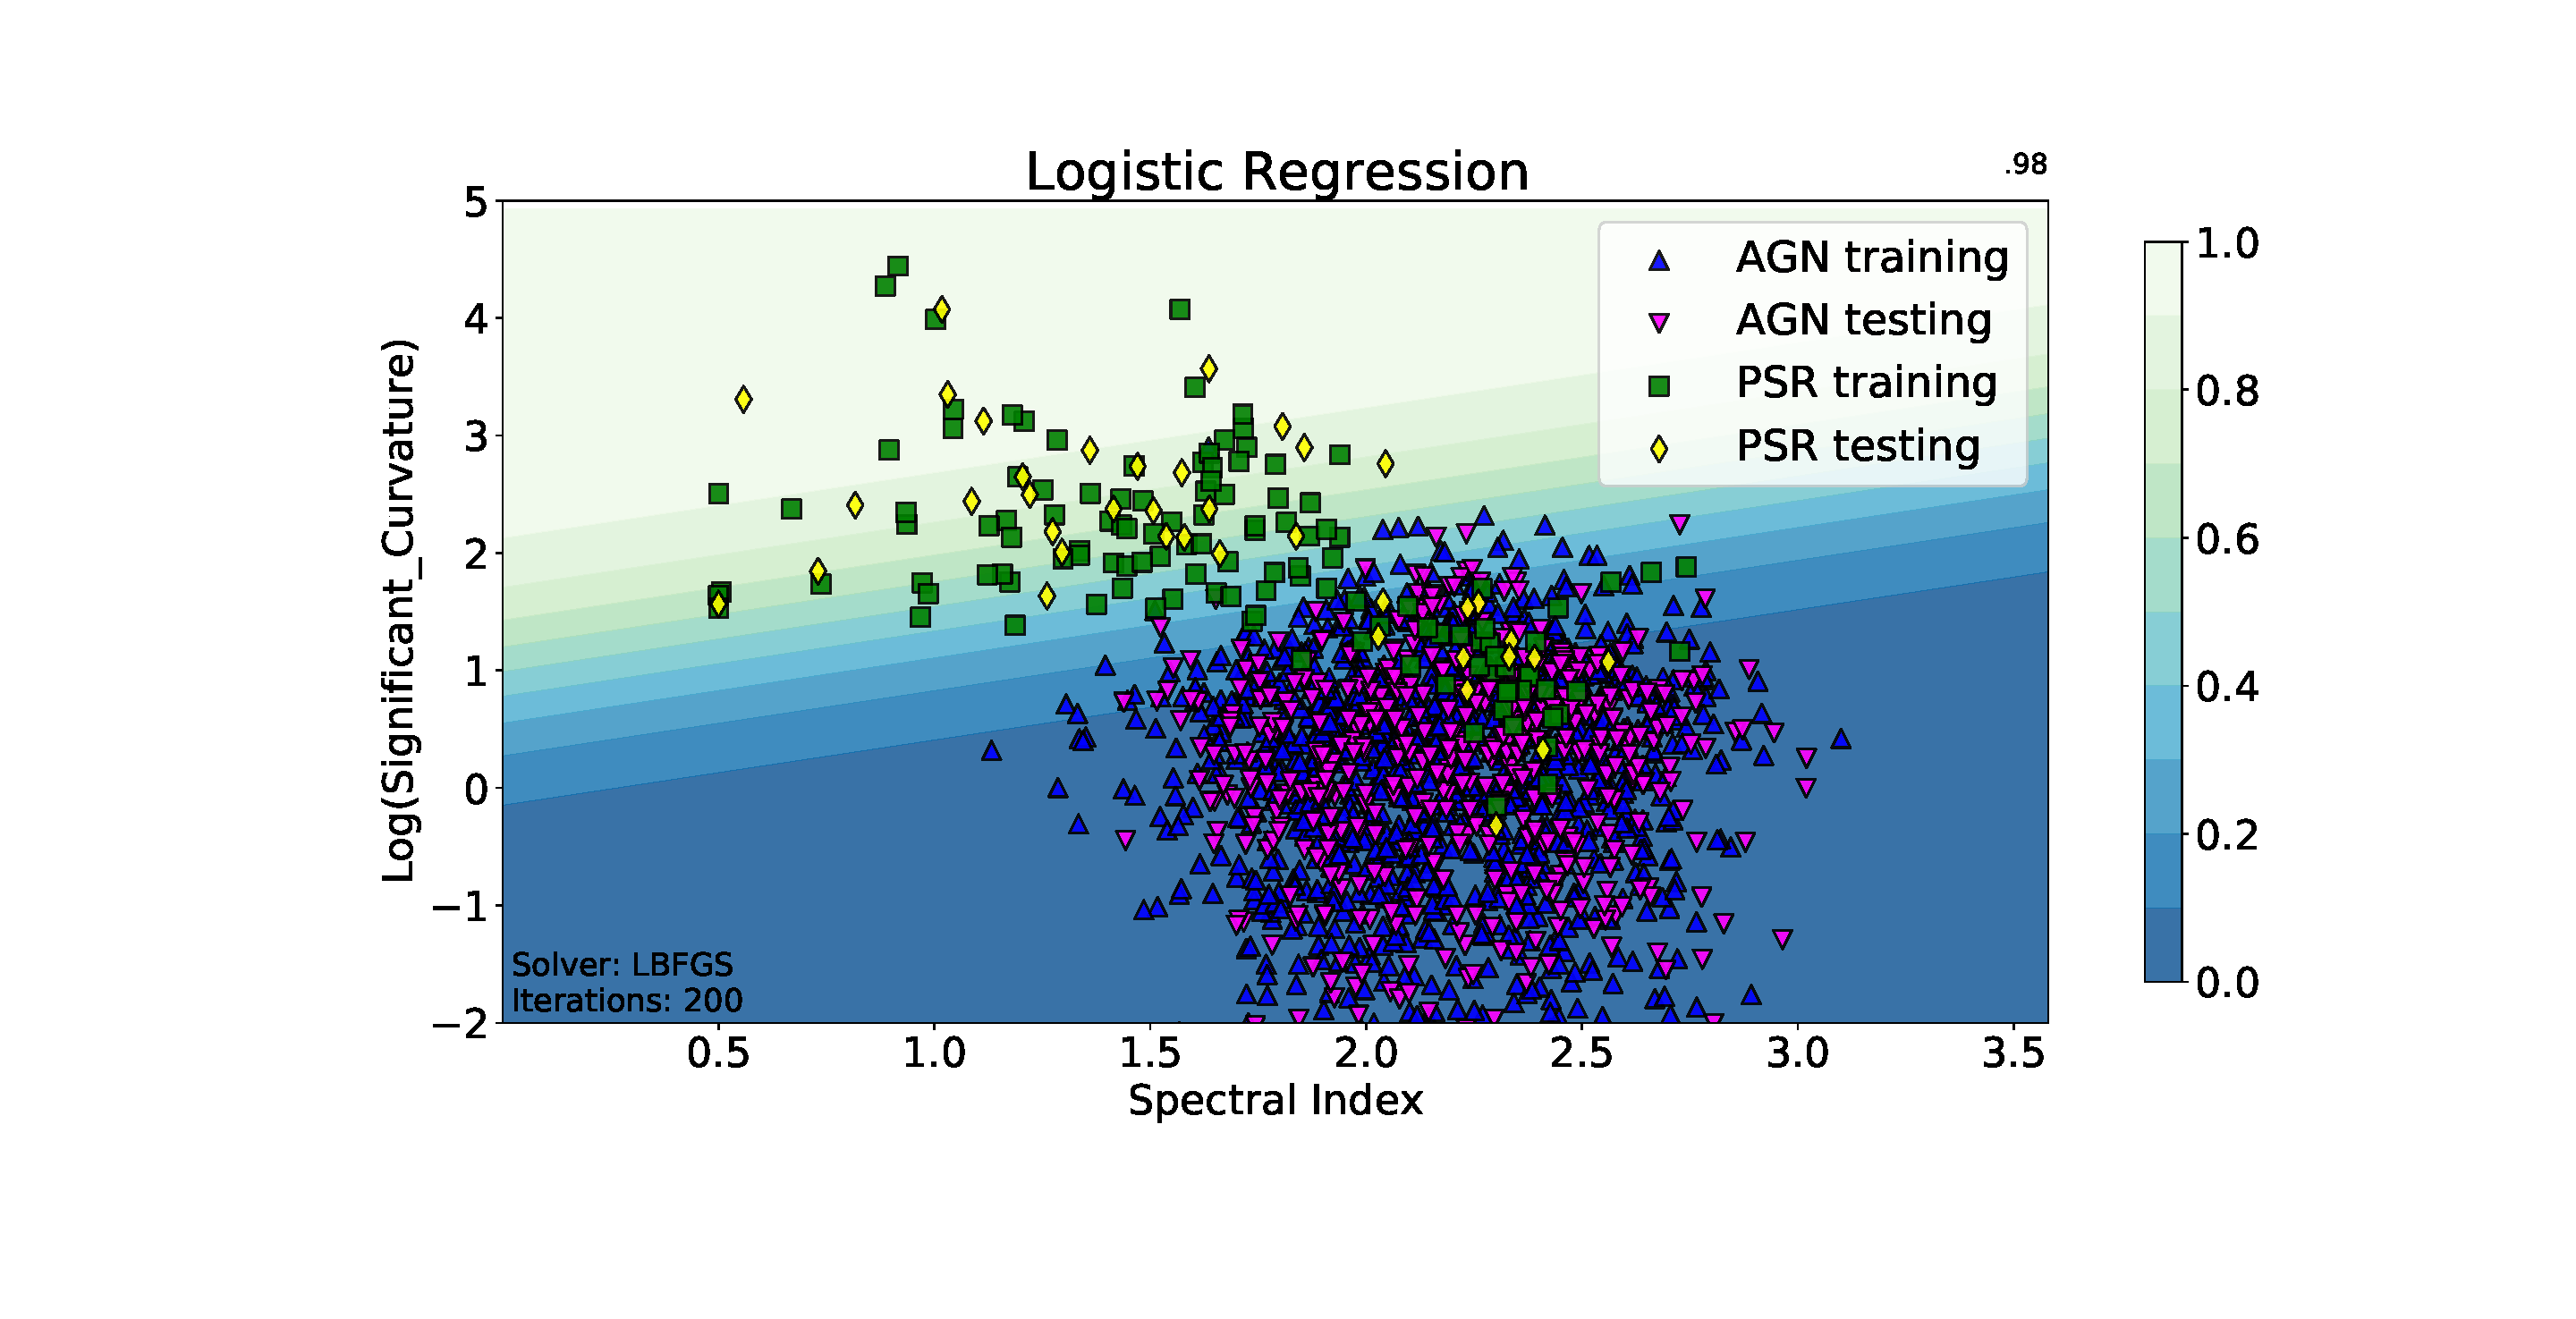
\includegraphics[width=0.5\textwidth]{plots/classification_domains/lr_200_lbfgs.pdf}
\caption{Top panel: LR classification domains showing class probabilities for training with oversampling.
The oversampling is illustrated by repeating the pulsar markers with a shift: the number of markers is equal to the number of times the pulsar appears in training.
Bottom panel: we repeat Fig. \ref{fig:LR_domains} for convenience of comparison with the oversampled training in the top panel.
In both panels the domains are obtained by averaging over 100 random splits into training and testing samples.
}  
\label{fig:LR_domains_O}
\end{figure}

\section{Probabilistic catalogs based on the 3FGL and 4FGL catalogs}
\lb{sec:prob_cats}

In this section we use the ML algorithms optimized in the previous section to construct probabilistic
classification of sources in the 3FGL and 4FGL catalogs.
%Having optimized our algorithms, we decided to test them on 3FGL data which was initially unassociated but then became associated in 4FGL. Furthermore, we tested the algorithms on 4FGL associated data, and also predicted for unassociated data.


\subsection{Probabilistic classification of sources in 3FGL and comparison with 4FGL}
\lb{sec:3FGLprediction1}


%In this section we perform probabilistic classification of sources in the 3FGL catalog.
We use the following four algorithms for the classification of sources: RF with 50 trees and maximal depth of 6, BDT with 100 trees and maximal depth of 2, NN with 11 neurons, LBFGS solver, and 300 epochs, and LR with LBFGS solver and 200 iterations. 
For training we use the pulsars and AGNs from the 3FGL catalog. In addition to original datasets, we perform oversampling of pulsars in order to balance the numbers of pulsars and AGNs.
As a result, we have 8 classification methods: 4 algorithms trained with and without oversampling.


\begin{table}[!h]
\hspace{-0.2cm}
\resizebox{0.47\textwidth}{!}{
    \tiny
  \centering
    \renewcommand{\tabcolsep}{0.4mm}
\renewcommand{\arraystretch}{1.6}

%\hspace{-3mm}
    \begin{tabular}{|c|c|c|c|c|c|c|}
    \hline
    Algorithm&Parameters &  Testing&Std. Dev.& Comparison with \\
    & & Accuracy & & 4FGL-DR2 Accuracy \\
    \hline
    RF & 50 trees, max depth 6  &97.37&0.60& 91.41  \\
    RF\_O &   &97.90&0.50& 90.28 \\
    \hline %\midrule   -> aakash do you mean this?
    BDT & 100 trees, max depth 2    &   97.65&0.54&90.64 \\
%    \hline %\midrule   -> aakash do you mean this?
%    BDT & 200 trees, max depth 2    &   95.8  \\
    BDT\_O &     &   97.79&0.51& 90.79 \\
    \hline
    NN & 300 epochs, 11 neurons, LBFGS & 97.29&0.97& 89.32\\
    NN\_O &  & 94.31&5.13& 85.99\\
    \hline
    LR & 200 iterations, LBFGS solver & 97.63&0.54& 89.97 \\
    LR\_O &  &93.68&0.99& 85.55\\
    \hline
     
    \end{tabular}}
    \vspace{2mm}
    \caption{Testing accuracy of the 4 selected algorithms for classification of 3FGL sources and comparison with associations in the 4FGL-DR2 catalog. 
    ``\_O'' denotes training with oversampling.}
    \label{tab:selected_algs}
\end{table}



\begin{figure}[h]
\centering
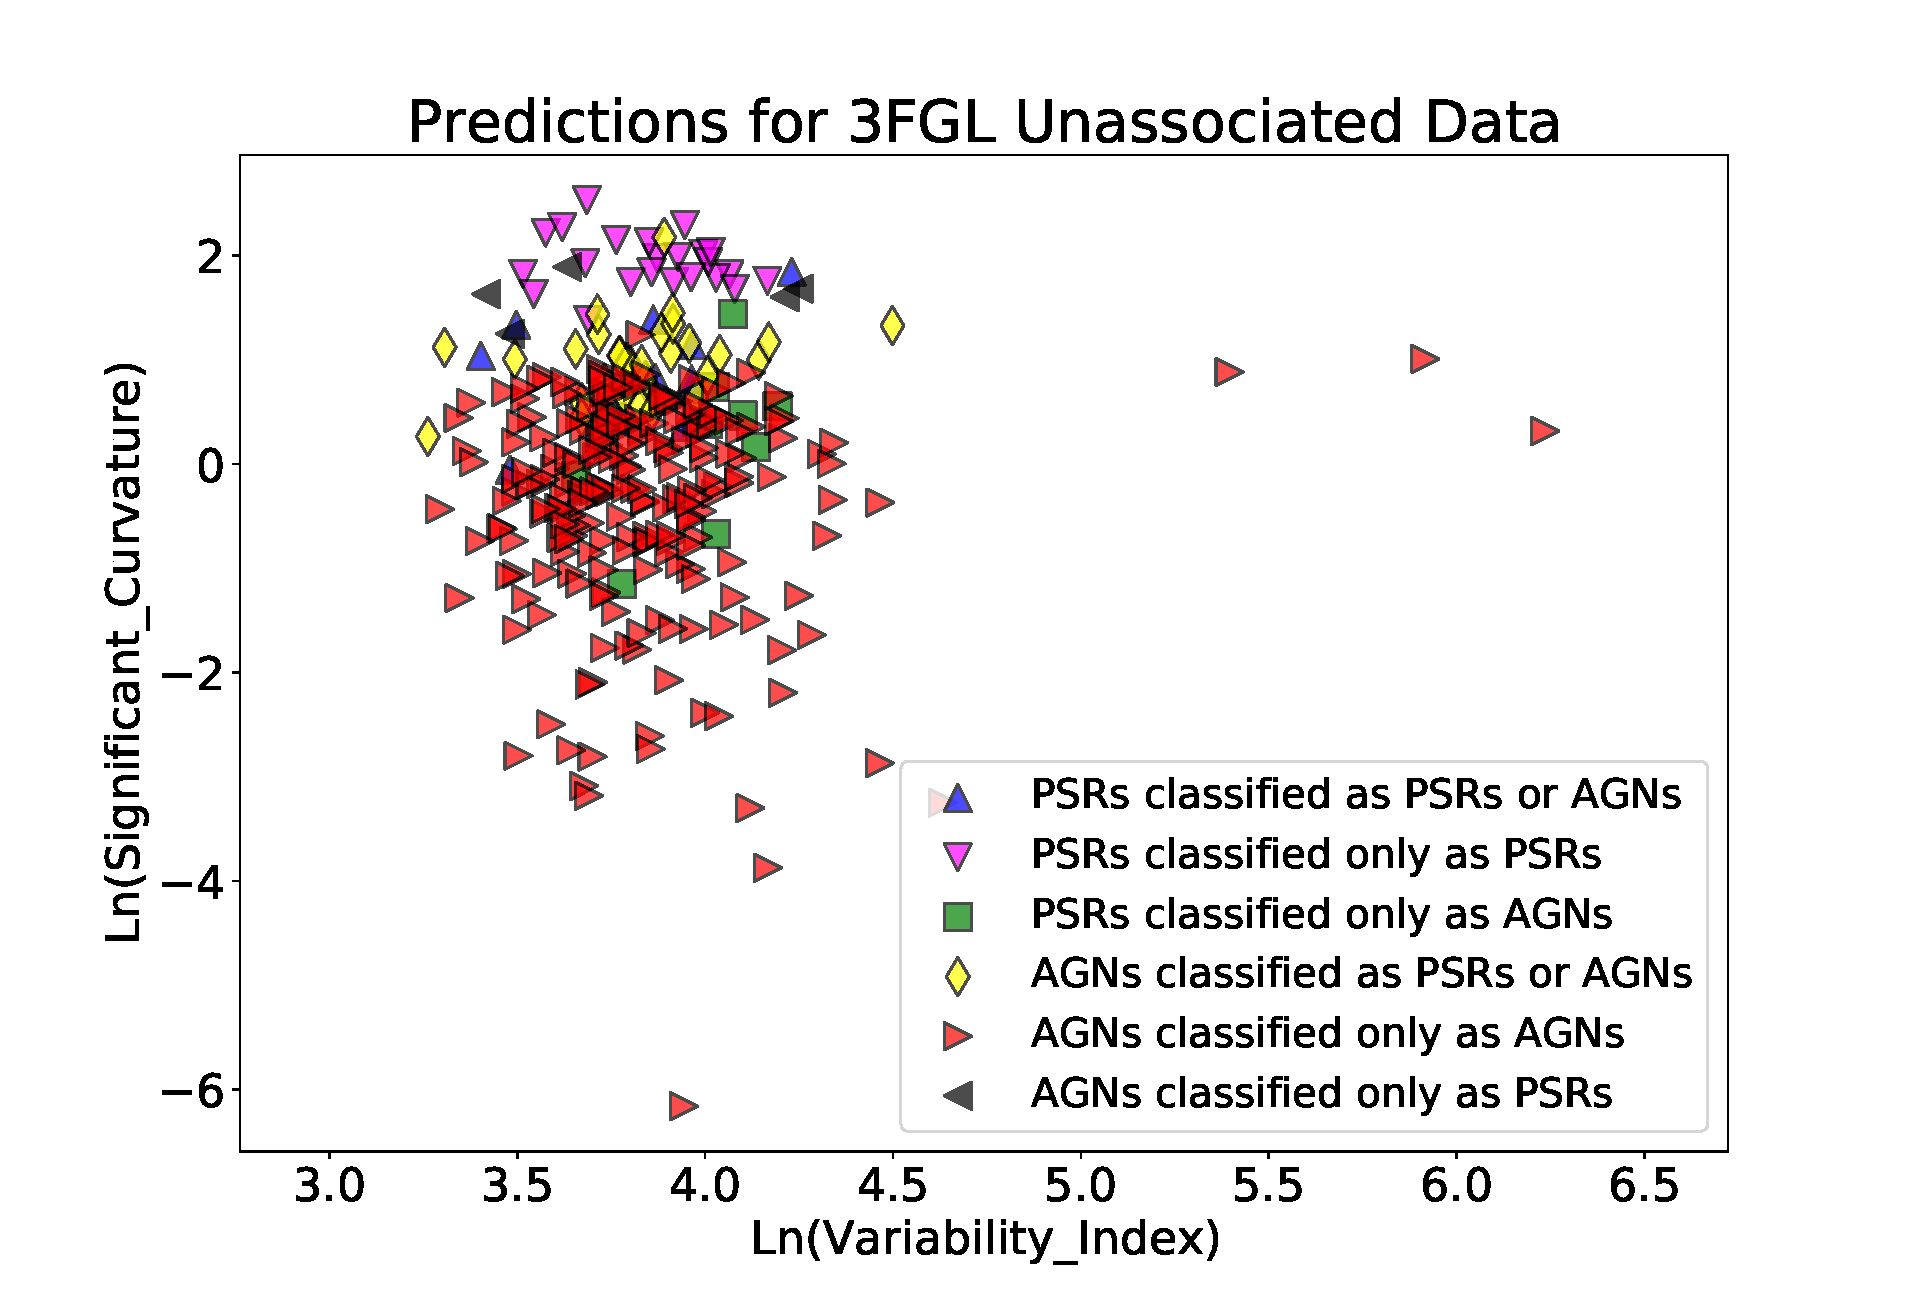
\includegraphics[width=0.48\textwidth]{plots/plot_final_DR2.pdf}
%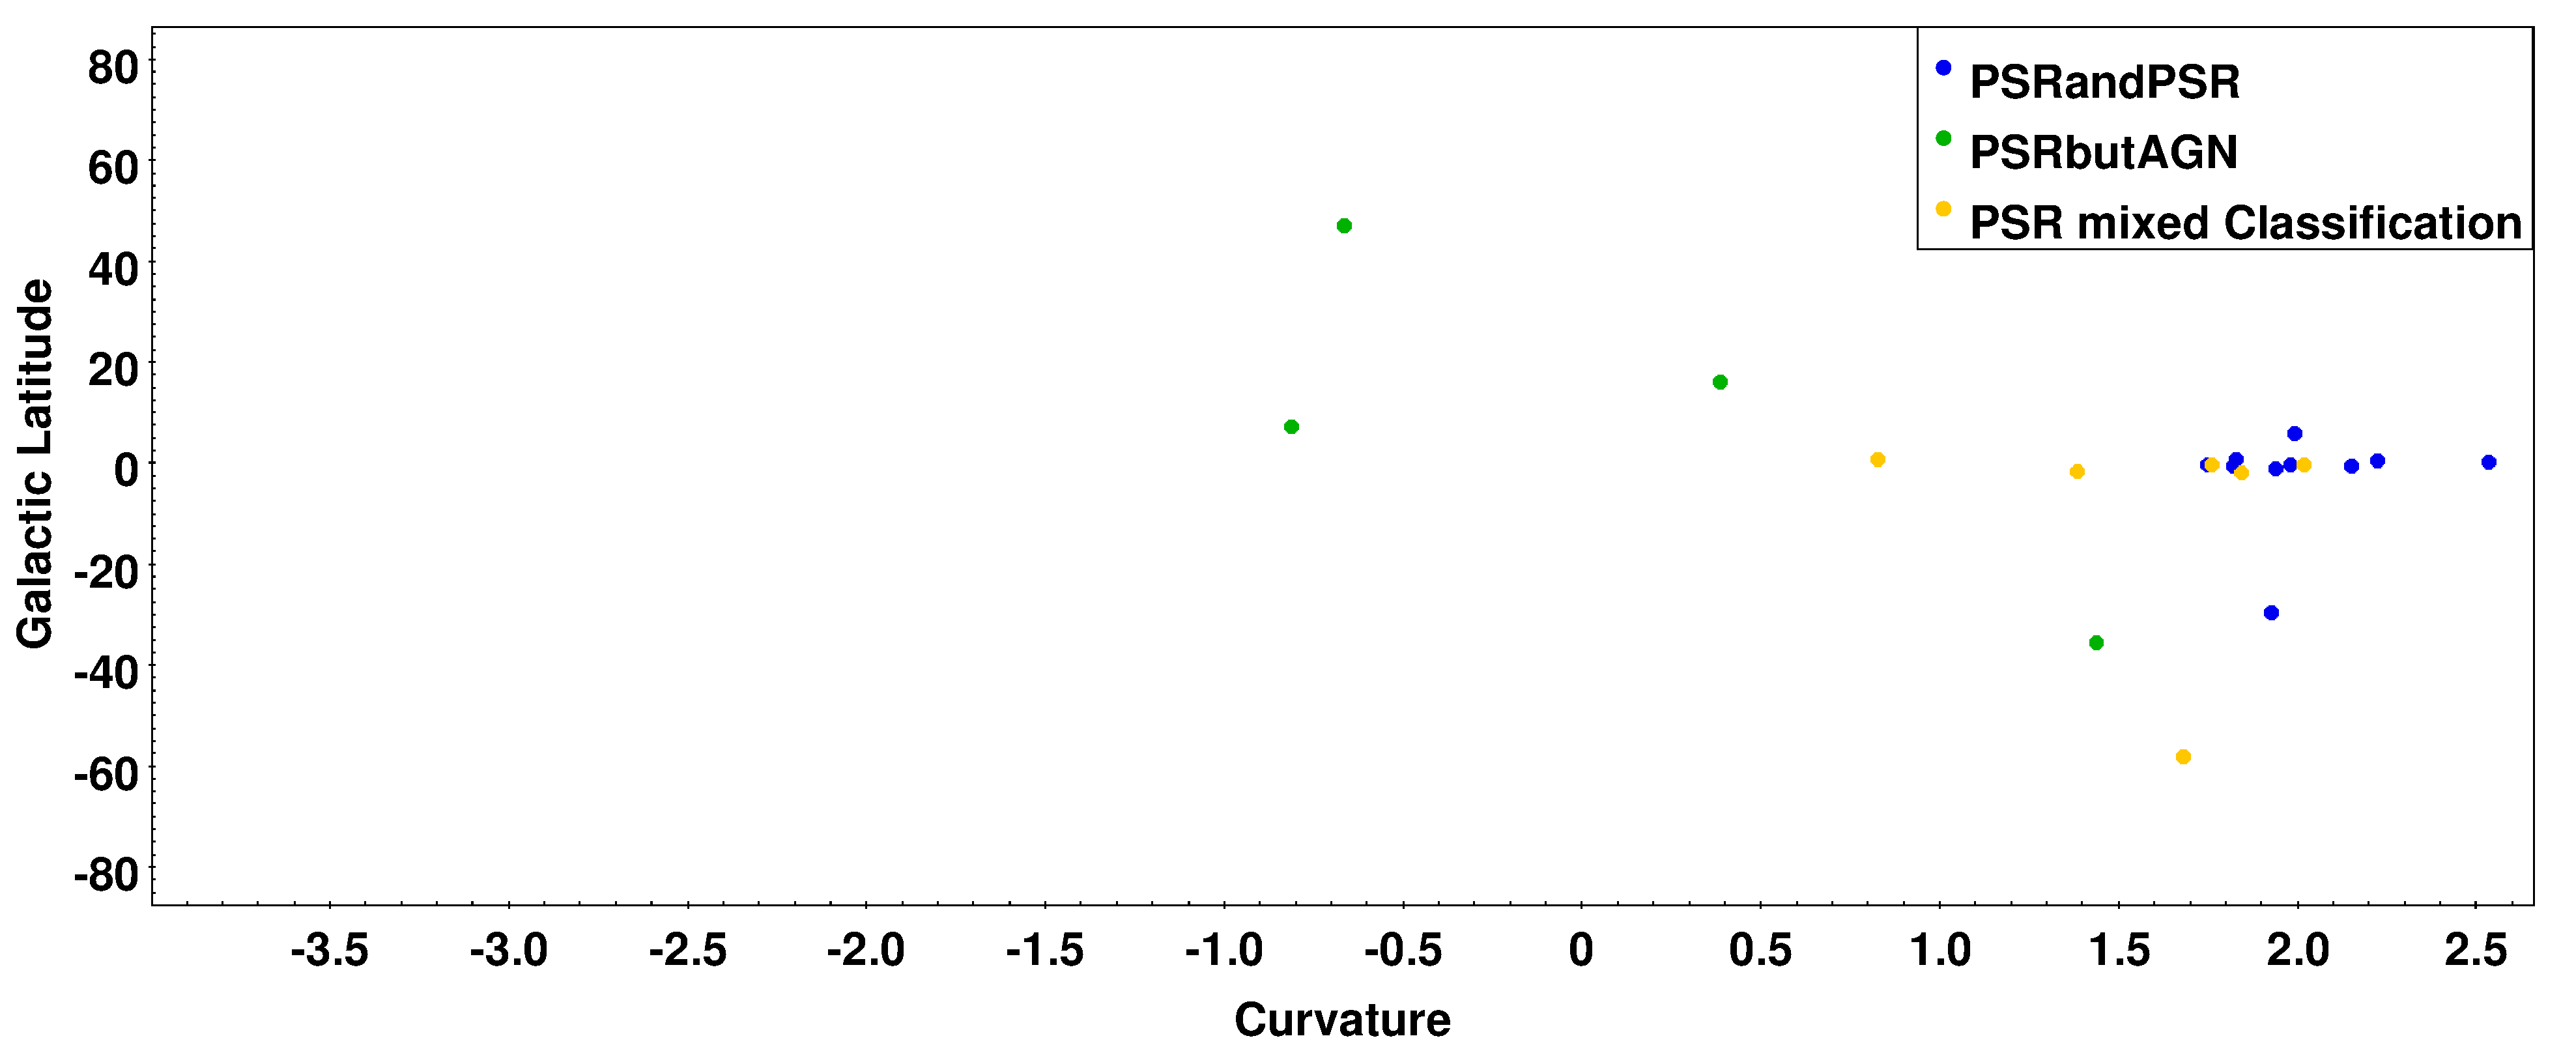
\includegraphics[width=\twopicsp\textwidth]{plots/PSR3.pdf}
\caption{Comparison of class prediction for unassociated 3FGL sources with classes in 4FGL-DR2. 
For more details see Section \ref{sec:3FGLprediction1}.}
%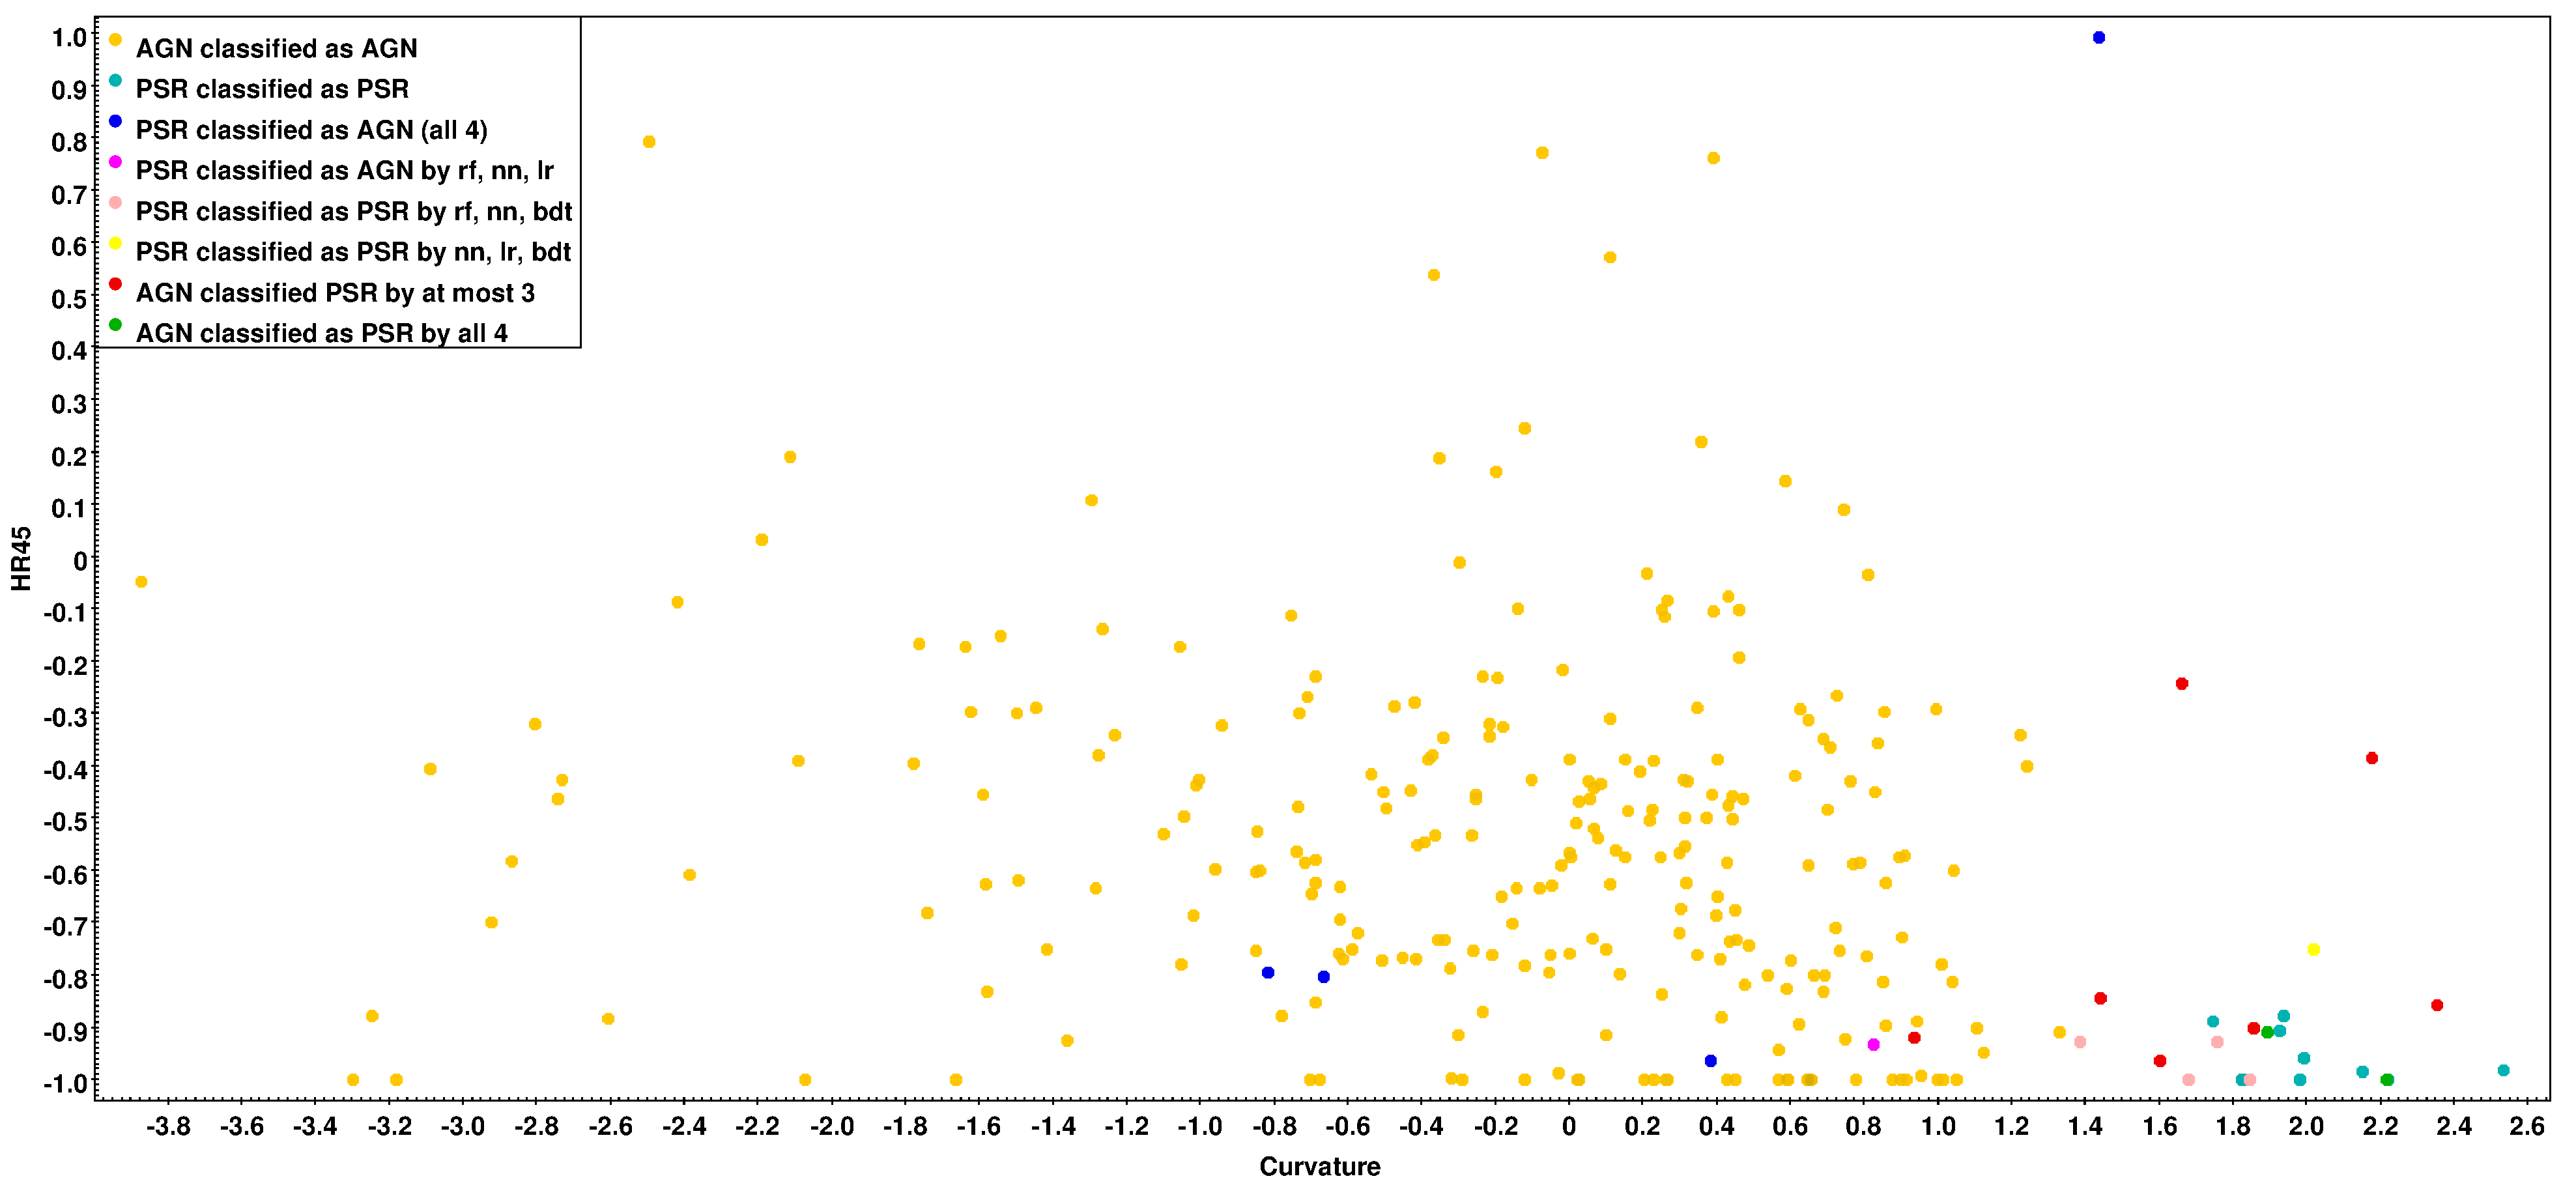
\includegraphics[width=\twopicsp\textwidth]{plots/final_catalog.pdf}
\label{fig:3FGL_vs_4FGL_classes}
\end{figure}

The selected algorithms are summarized in Table \ref{tab:selected_algs}, where oversampling is shown by ``\_O''.
``Average testing accuracy'' is computed by taking 1000 times 70\% - 30\% split into training and testing samples and averaging over the 
accuracies computed for the testing samples.
In addition, we look at sources, which are unassociated in 3FGL but have either pulsar or AGN association in 4FGL-DR2: there are 302 such sources.
The accuracy of our prediction for the four selected algorithms with and without oversampling, taking the 4FGL-DR2 classes as the true values, is reported in the column ``Comparison with 4FGL Accuracy''.
The correct classifications and misclassifications for the 302 sources with PSR or AGN associations in 4FGL-DR2 are also presented in Figure \ref{fig:3FGL_vs_4FGL_classes}.
The class at the beginning of the label name corresponds to the association in the 4FGL-DR2, while the second half of the labels corresponds to classification of unassociated sources in 3FGL. For example, ``PSRs classified only as PSRs'' shows sources which have PSR association in 4FGL-DR2 and all eight methods classified the corresponding unassociated sources in 3FGL as a pulsar. ``PSRs classified as either PSRs or AGNs'' labels sources with PSR associations in 4FGL-DR2 but the corresponding unassociated sources in 3FGL have both PSR and AGN classifications by different ML methods.
The unassociated sources are classified as PSRs or AGNs if the corresponding probability is larger than 0.5.
We notice that misclassified or partially misclassified sources in Figure \ref{fig:3FGL_vs_4FGL_classes} typically happen on the boundary between the two classes or even inside the opposite class.
Many of these sources also have flags in the 3FGL catalog, such as a potential problem with the background diffuse emission model in the location of the source, which can lead to a poor reconstruction of the source spectrum and, consequently, misclassification of the source.


As a result of the classification with the eight ML methods,
we created a probabilistic catalog based on the 3FGL sources without missing values.%
\footnote{There are thirteen sources with missing values in the 3FGL catalog (2 unassociated, 5 AGNs, 1 pulsar, and 5 ``other'' sources), 
which we save in a separate file ``3FGL\_sources\_with\_missing\_values.csv'' for reference. In particulat all of these sources have a value in significant curvature of 0.
%\dima{Which features are missing for these sources, could we still classify them?}
}
We train on 70\% of the sources associated with pulsars or AGNs and save the probability values for testing sources, for sources which are not classified as pulsars or AGNs, and for unassociated sources.
We repeat the splitting and training 1000 times and report the sample average and standard deviation of the classification probabilities,
i.e., we average over 1000 values for unassociated sources and sources not classified as AGNs or pulsars, 
while the average for AGNs and pulsar is over the number of times the sources appear in the testing sample, which is 300 on average.
%Like in the case of associated sources, where we split the data 1000 times, we also do a 1000 runs for the unassociated case. This allows us to calculate individual probabilities and their standard deviations for all sources.
%\dima{Classification of associated sources is done by averaging over testing-training samples splits.
%Do we also do averaging for unassociated sources?}
We have also subselected the 302 unassociated 3FGL sources, which have PSR or AGN associations in 4FGL-DR2,
and saved them for convenience of comparison as a separate file.

In the probabilistic catalogs we add columns with corresponding probabilities for each algorithm and each class,
i.e., provided that there are 8 methods (including oversampling) and 2 classes, we add 16 columns: 8 for unweighted and 8 for oversampled training data. The columns with '\_O' represent the oversampled probabilities. We also add 16 columns for standard deviations of probabilities. Although class probabilities and standard deviation for each algorithm are not independent (probabilities add up to 1 and standard deviations are equal for AGN and PSR classes), we keep the corresponding columns in view of the generalizations to multi-class classification (e.g., 3-class classification in Section \ref{sec:3class}).
%Although the class probabilities for each algorithms should add up to one for every source, we still keep the columns for all classes for convenience.
Table \ref{tab:prob_cat} shows an example of the probabilistic catalog for a few unassociated 3FGL sources.
Notice that the first source is classified as a pulsar by BDT and as an AGN by RF, LR, and NN algorithms,
it is an example of a source with mixed classification.
%i.e., it has a label ``classified either as PSRs or AGNs'' in Figure \ref{fig:3FGL_vs_4FGL_classes}. - is it associated in 4FGL?
%The second and third sources are classified as AGNs by all four algorithms, i.e., they will have a label ``classified only as AGNs'',
%while the last source is classified as a pulsar by all four algorithms, i.e., it will have a label ``classified only as PSRs''.
Out of 1008 unassociated sources in 3FGL, 111 are classified as pulsars by all eight methods, 597 are classified as AGNs, and 300 have mixed classifications.
Out of 111 sources classified as pulsars, 6 sources have counterparts in Parkes survey \citep{Camilo2015} within 2 arc minutes (see Table \ref{tab:parkes}).

We summarize the results of classification of unassociated sources in Table \ref{tab:prediction_2and3class} in the ``2-class'' row.
The ``AGNs'' column shows the number of unassociated sources where all eight methods from Table \ref{tab:selected_algs} 
give the probability for a source to be an AGN above 50\%.
Similarly the ``Pulsars'' column shows the number of unassociated sources where all algorithms predict the source to be more likely a pulsar.
The ``Mixed'' column shows the number of sources with mixed classification, i.e., some algorithms predict that the source is more likely an AGN while the other algorithms predict that it is more likely a pulsar.
We also add the ``OTHER'' column in order to compare the results with the 3-class classification later in this Section.
Since there is no ``OTHER'' class in the 2-class classification, the corresponding entry is empty.
In the ``2-class corr'' row we show a possible correction of the number of pulsars and AGNs due to presence of other sources.
Here we assume that the fraction of AGN-like and pulsar-like sources among the other sources is the same for associated and for unassociated sources.
In particular, if we denote by $N_{\rm AGN}$ the number of unassociated sources with AGN-like probabilistic classification,
by $N_{\rm AGN}^{\rm ass\,OTHER}$ the number of sources with AGN-like classification among associated OTHER sources,
by $N_{\rm ass}$ ($N_{\rm unass}$) the total number of associated (unassociated) sources, then
the number of AGN-like sources among the unassociated ones corrected for the presence of OTHER sources can be estimated as

\be
\lb{eq:other_correction}
N_{\rm AGN}^{\rm corr} = N_{\rm AGN} - N_{\rm AGN}^{\rm ass\,OTHER} \,\frac{N_{\rm unass}}{N_{\rm ass}}.
\ee
Analogous corrections are applied for the number of unassociated sources with PSR and with mixed classifications.
If we denote by $N^{\rm ass\,OTHER}$ the total number of associated other sources, then the estimated number of 
OTHER sources among unassociated ones is
\be
\lb{eq:2class_other}
N^{\rm unass}_{\rm OTHER} = N^{\rm ass\,OTHER} \,\frac{N_{\rm unass}}{N_{\rm ass}}.
\ee
We show this estimate in the OTHER column in the ``2-class corr'' row.
We note that since 
$N_{\rm AGN}^{\rm ass\,OTHER} + N_{\rm PSR}^{\rm ass\,OTHER} + N_{\rm MIXED}^{\rm ass\,OTHER} = N^{\rm ass\,OTHER}$,
this estimate is consistent with corrections in Equation (\ref{eq:other_correction}) for sources classified as AGNs, pulsars, or with mixed classification.


\pgfplotstableread[col sep=comma]{tables/3FGL_unassoc_vs_4FGL_assoc.csv}\loadedtable
\begin{table}
\pgfplotstabletypeset[columns={Source_Name_3FGL,AGN_BDT,AGN_RF,AGN_LR,AGN_NN},
column type=l,
string type,
every head row/.style={before row={\toprule & \multicolumn{4}{c}{AGN Probability} \\},after row=\midrule,},
every last row/.style={after row=\midrule}, %\vdots },
columns/Source_Name_3FGL/.style={column name=Source\_Name\_3FGL},
columns/AGN_BDT/.style={column name=BDT,numeric type,fixed,precision=3},
columns/AGN_NN/.style={column name=NN,numeric type,fixed,precision=3},
columns/AGN_RF/.style={column name=RF,numeric type,fixed,precision=3},
columns/AGN_LR/.style={column name=LR,numeric type,fixed,precision=3},
skip rows between index={4}{302}
]\loadedtable
\caption{\label{tab:prob_cat}
Example of the AGN classification probabilities for a few unassociated sources in the 3FGL catalog \citep{2015ApJS..218...23A}. We have ommited the oversampled probability columns here.}
\end{table}




\pgfplotstableread[col sep=comma]{tables/3fgl_unassoc_predictions_matches_with_Parkes(2015)_1.csv}\loadedtable
\begin{table}
\pgfplotstabletypeset[columns={Source_Name_3FGL,GLON,GLAT,Separation},
column type=l,
string type,
every head row/.style={before row={\toprule},after row=\midrule,},
every last row/.style={after row=\midrule },
columns/Source_Name_3FGL/.style={column name=Source\_Name\_3FGL},
columns/GLON/.style={column name=GLON,numeric type,fixed,precision=1},
columns/GLAT/.style={column name=GLAT,numeric type,fixed,precision=1},
columns/Separation/.style={column name=Sep (arksec),numeric type,fixed,precision=1}
]\loadedtable
\caption{\label{tab:parkes}
Connection of unassociated 3FGL sources classified as pulsars with Parkes pulsars \citep{Camilo2015}.}
\end{table}




\subsection{Probabilistic classification of sources in the 4FGL-DR2 catalog}
\lb{sec:4FGLprediction}

In this section we construct a probabilistic classification of sources in the 4FGL-DR2 catalog. The 4FGL-DR2 catalog \citep{2020arXiv200511208B} 
is based on 10 years of \Fermi-LAT data \citep[compared to 8 years of data in the 4FGL catalog,][]{2020ApJS..247...33A}.
It contains 5788 sources, which is 723 sources more than in the 4FGL catalog (all sources in 4FGL are kept in 4FGL-DR2 even if they fall
below the detection threshold with 10 years of data). 
3770 sources in 4FGL-DR2 have either an  AGN or a PSR classification, 
1658 sources are unassociated (we only look at CLASS1 column in the catalog), and the rest 346 sources are other sources with classification like PWN, SNR, etc.
There are 14 sources in 4FGL-DR2 with missing values: four AGNs, one PWN (Crab), and nine unassociated sources.
As in the previous section, we use for training and testing sources associated with either AGNs or pulsars,
which have no missing values used for classification.
%\footnote{In the 4FGL catalog there is only one source with missing values: 4FGL J0534.5+2201i associated with the Crab pulsar wind nebula.}
We then calculate the classification probabilities of AGN and PSR classes for both the associated and the unassociated sources.
The 4FGL catalog has higher number of features, especially due to the difference in modeling of the spectra compared with the 3FGL catalog. 
We selected 28 of these features and looked for correlations among them. If any feature was correlated or anti-correlated with a Pearson index of $\pm$0.75 or higher with another feature, then only one of these features was kept. 
%The correlation matrix is shown in Figure \ref{fig:corr_mat}.
The resulting 10 features are:
GLON, GLAT, ln(Pivot\_Energy), ln(Energy\_Flux100), ln(Unc\_Energy\_Flux100), LP\_Index, Unc\_LP\_Index, LP\_beta, LP\_SigCurv, ln(Variability\_Index).
In addition similar to the classification of the 3FGL sources, we add 6 hardness ratios to the list of features:
hr12, hr23, hr34, hr45, hr56, hr67 (in the 4FGL-DR2 catalog there are two more energy bins compared to the 3FGL catalog).
Thus, in total we use 16 features for classification of 4FGL-DR2 sources.
%Some of these features are direct counterparts to the features which we used in the 3FGL catalog, e.g., GLAT, LP\_Index (instead of 500MeV\_Index), LP\_SigCurv (instead of ln(Signif\_Curve)), ln(Variability\_Index), hardness ratios.

\begin{comment}
\begin{figure*}[h]
\centering
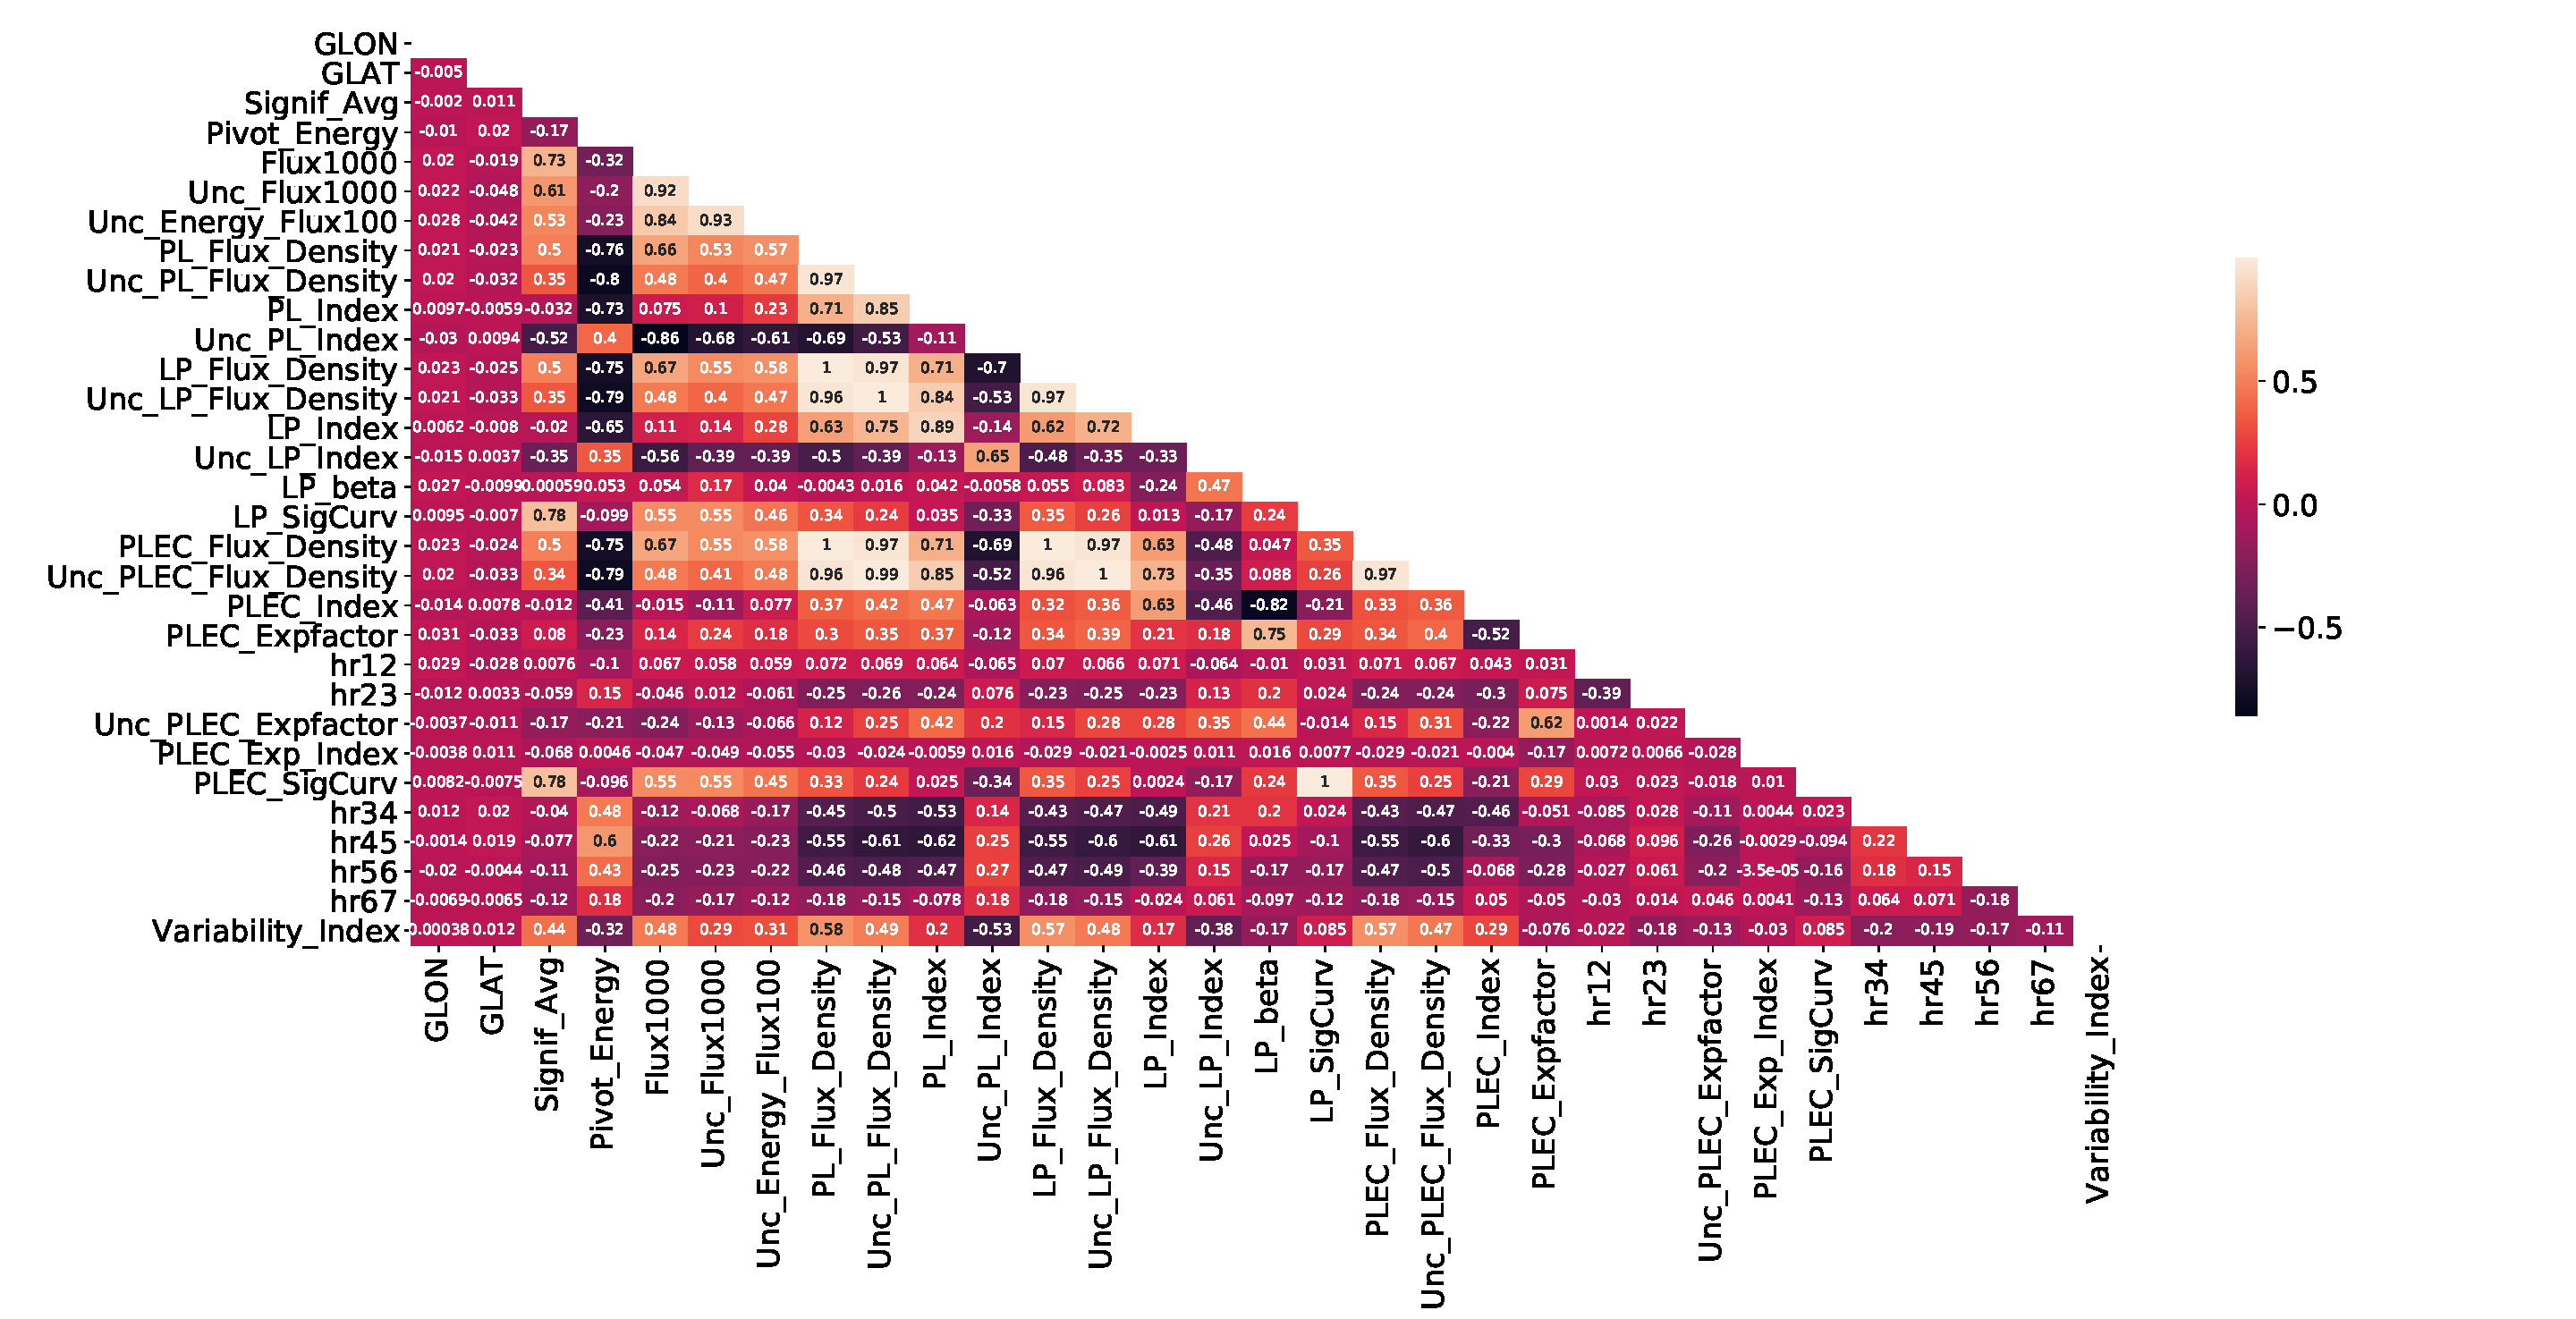
\includegraphics[width=\textwidth]{plots/correlation_4fgl_assoc.pdf}
%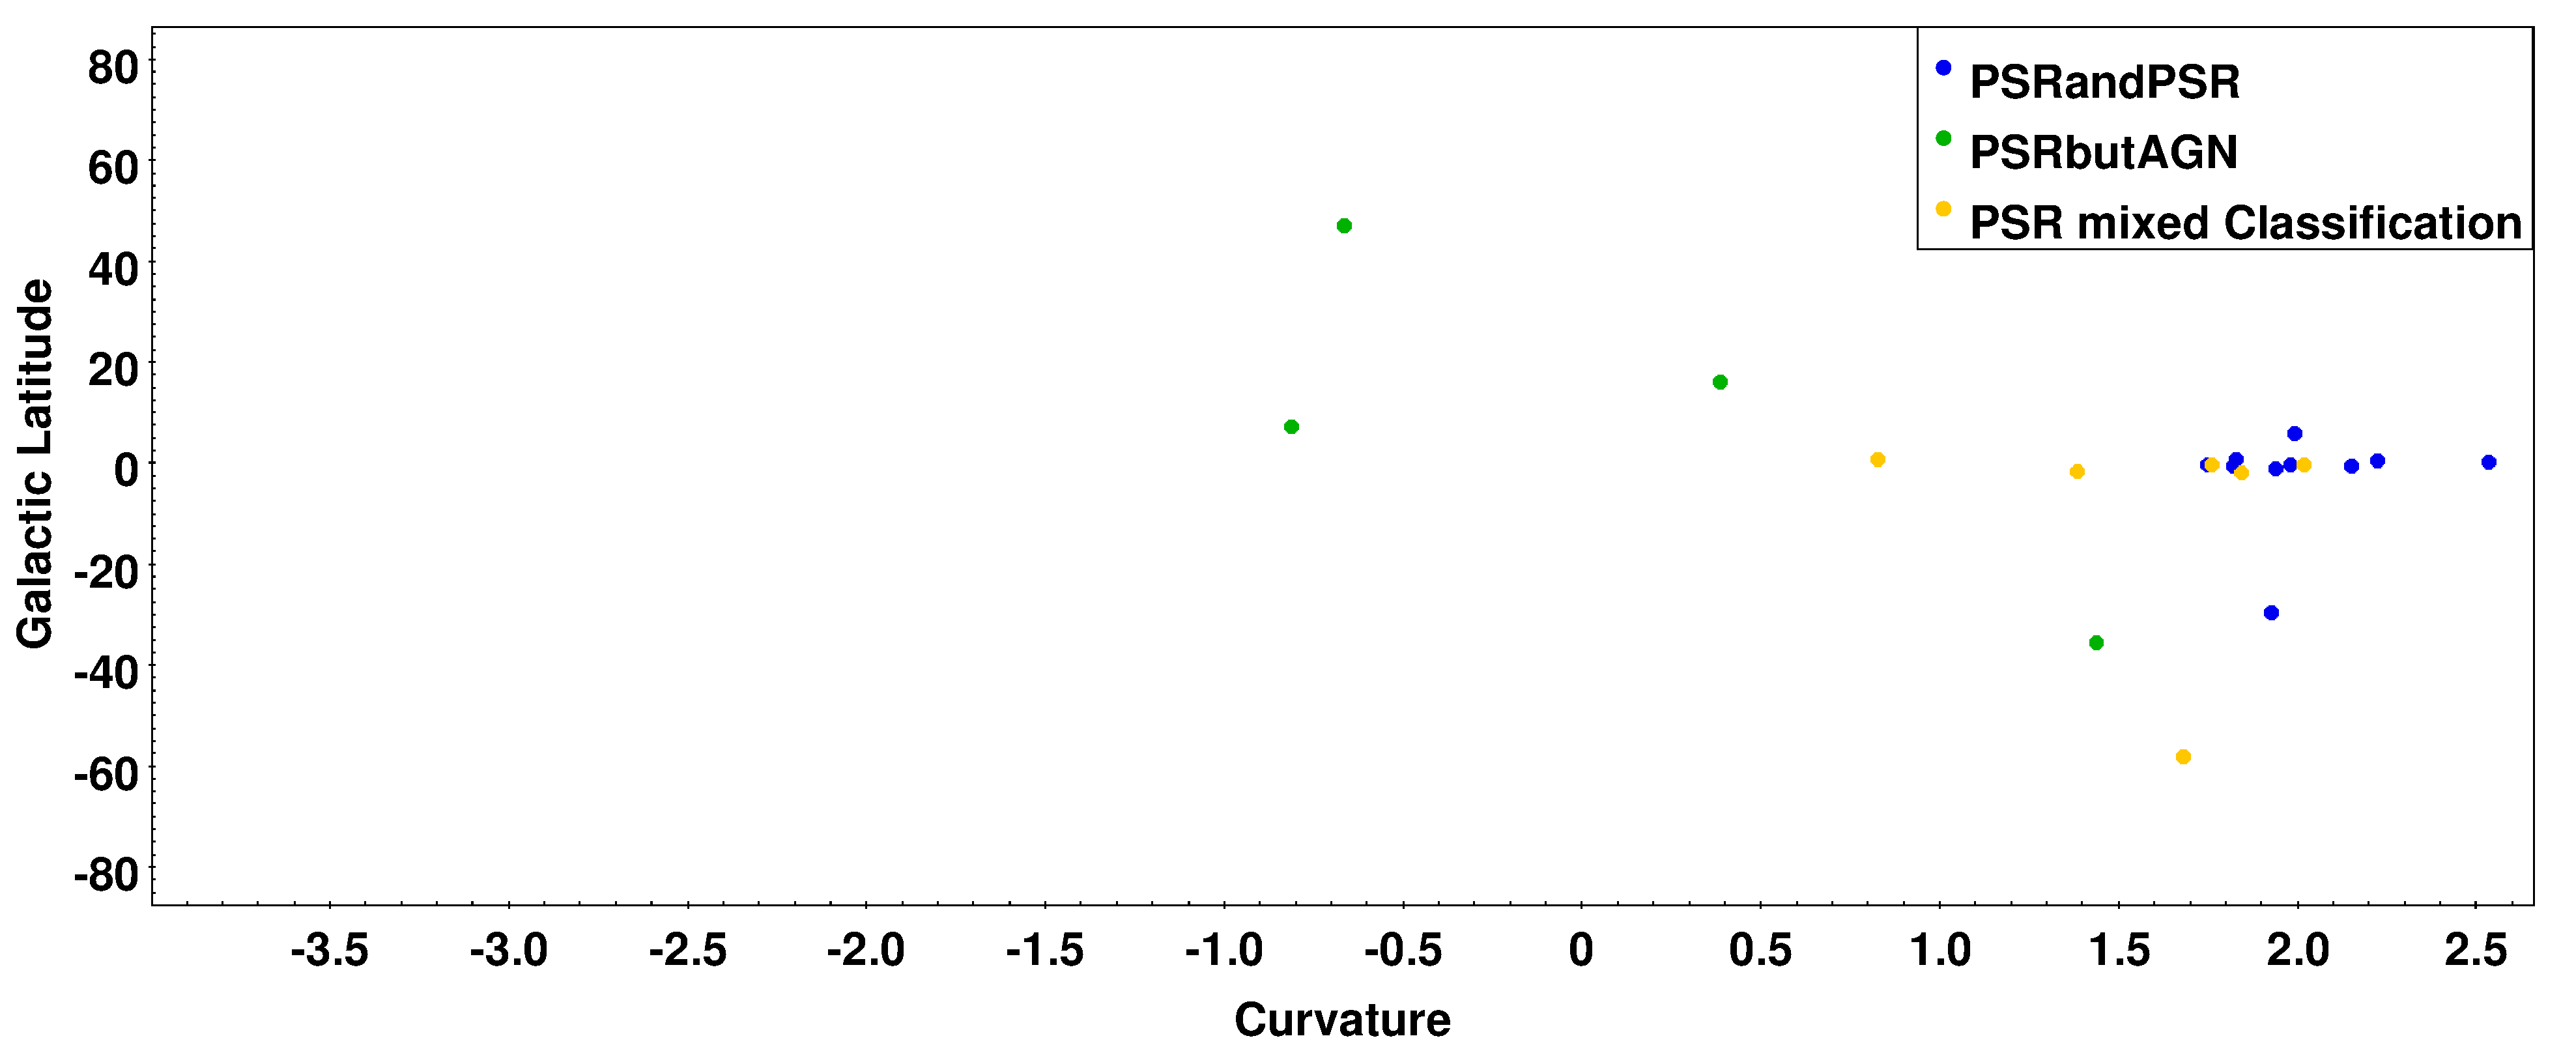
\includegraphics[width=\twopicsp\textwidth]{plots/PSR3.pdf}
\caption{Corelation matrix for 4FGL-DR2 associated data }
%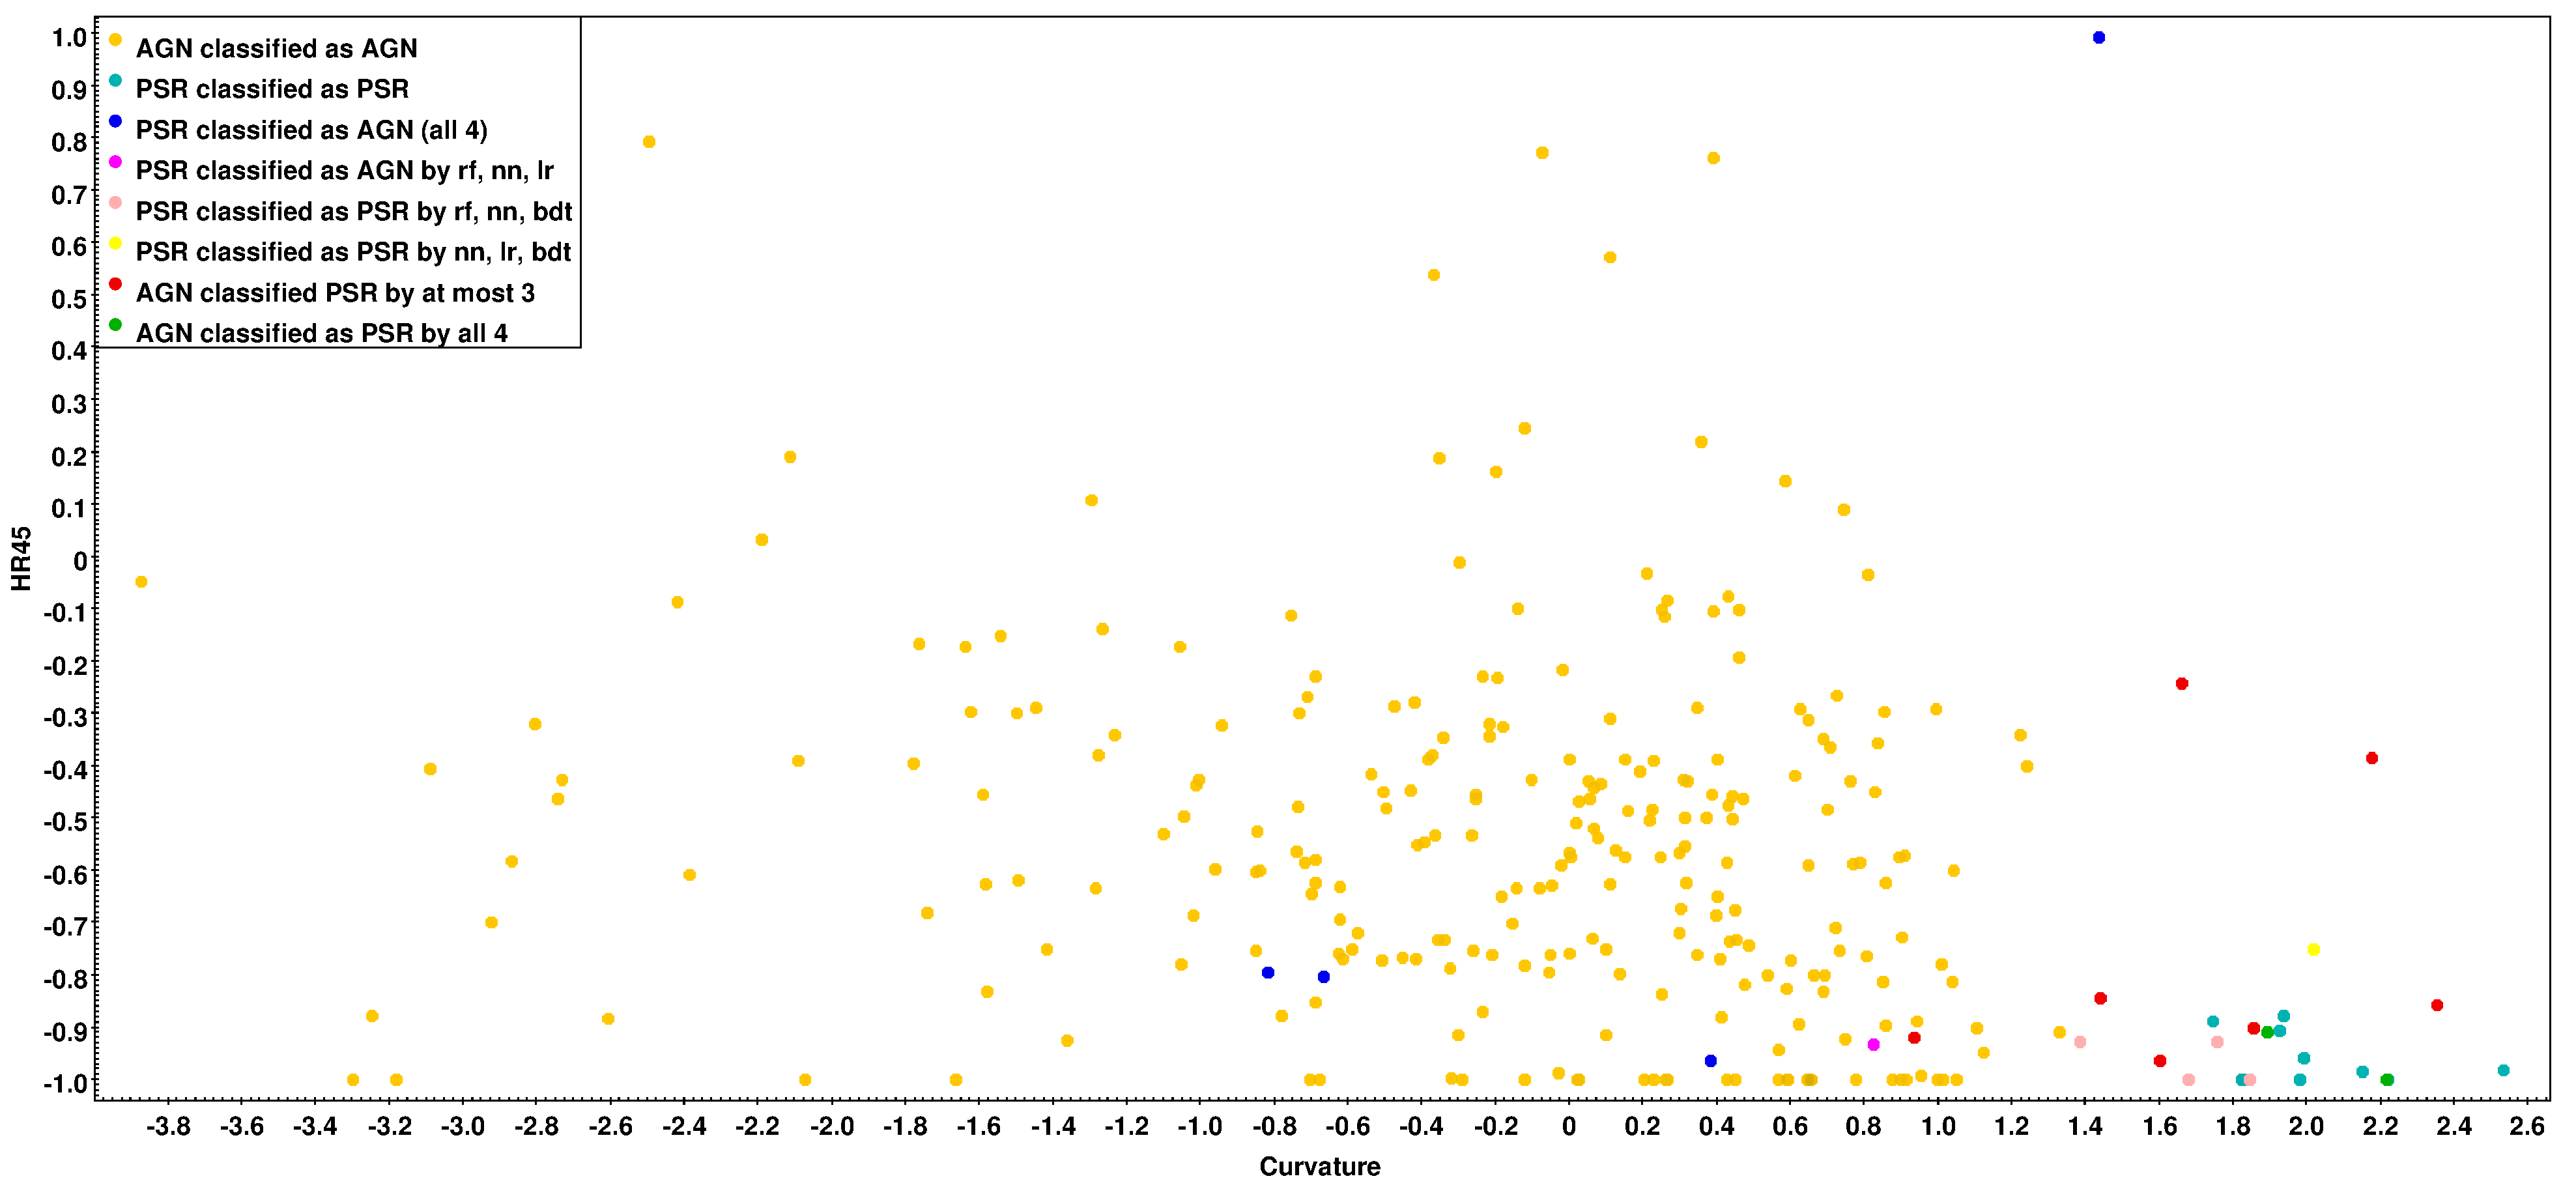
\includegraphics[width=\twopicsp\textwidth]{plots/final_catalog.pdf}
\label{fig:corr_mat}
\end{figure*}
\end{comment}

For the classification of 4FGL-DR2 sources, we confirmed that the parameters used in 3FGL classification provide an optimal performance for the 4FGL-DR2 catalog as well.
Therefore, we used the same meta-parameters for the four algorithms as in the construction of the probabilistic catalog based on 3FGL, except for NN where we increased the number of neurons in the hidden layer to 16. Similar to the construction of the 3FGL probabilistic catalog, we use both unweighted training samples and oversampling, i.e., we have 8 classification methods.
We retrain the algorithms using the 16 features for the 4FGL-DR2 sources.
The corresponding accuracies are reported in Table \ref{tab:selected_algs2}.
All algorithms have a slightly better accuracy for the 4FGL-DR2 catalog compared to the 3FGL catalog, which is likely due to a better determination of the spectra in 4FGL-DR2, to a higher number of features, and more associated sources used as training data. 

% (same as the number of features). However, due to the number of features being higher, we hypothesized that the Neural Network should under-perform as compared to before.

\begin{table}[!h]
\resizebox{0.45\textwidth}{!}{
    \tiny
 %  \centering
    \renewcommand{\tabcolsep}{0.4mm}
\renewcommand{\arraystretch}{1.6}

    \begin{tabular}{|c|c|c|c|}
    \hline
    Algorithm&Parameters & Testing Accuracy & Std. Dev.\\
    \hline
    RF& 50 trees, max depth 6  &97.87 & 0.36\\
    RF\_O   &&97.56&0.39 \\
    \hline %\midrule   -> aakash do you mean this?
    BDT & 100 trees, max depth 2    &   97.63 &0.39\\
    BDT\_O&&97.72&0.38\\
    \hline
    NN & 300 epochs, 16 neurons, LBFGS  & 97.41 & 0.47\\
    NN\_O&&95.48&0.66\\
    \hline
    LR & LBFGS solver, 200 iterations & 97.80&0.38\\
    LR\_O&&96.03&0.53\\
    \hline
     
    \end{tabular}}
    \vspace{0.2cm}
    \caption{Testing accuracy of the 4 algorithms on 4FGL-DR2 associated data. ``\_O'' denotes training with oversampling.}
    \label{tab:selected_algs2}
\end{table}

The expected numbers of pulsars and AGNs among the 1658 unassociated sources in 4FGL-DR2 without missing values are
presented in the 4FGL-DR2 part of Table \ref{tab:prediction_2and3class}.
The definition of rows is the same as in the 3FGL catalog 2-class classification in Section \ref{sec:3FGLprediction1}.


\begin{table}[!h]
\resizebox{0.45\textwidth}{!}{
    \tiny
 %  \centering
    \renewcommand{\tabcolsep}{0.3mm}
\renewcommand{\arraystretch}{1.5}

    \begin{tabular}{| l |c|c|c|}
    \hline
    Correction for other sources & AGNs & Pulsars & Mixed \\
    \hline
    Uncorrected &  872 & 162  &  624 \\
    \hline
    Corrected & 820.8  & 134.6  & 563.2 \\
    \hline
     
    \end{tabular}}
    \vspace{0.2cm}
    \caption{Expected numbers of pulsars and AGNs among unassociated sources in the 4FGL-DR2 catalog \citep{2020arXiv200511208B}.
    For definitions see Table \ref{tab:3FGL_prediction}.}
    \label{tab:4FGL-DR2}
\end{table}


Finally, we looked at sources which were unassociated in both 3FGL and 4FGL-DR2 (using 'ASSOC\_FGL' as an identifier for 3FGL sources). Out of 303 such sources\footnotetext{These are actually 303 4FGL-DR2 sources and 302 3FGL sources with 2 4FGL-DR2 sources associated with 1 3FGL source.}, 40 sources are predicted to be pulsars using 3FGL features and 75 sources are predicted to be pulsars using 4FGL features. This leads to 29 sources which are predicted by all eight methods to be pulsars for features taken from both 3FGL and 4FGL catalogs. 
For convenience, we save these 29 pulsar candidates as a separate file.

Among the 6 unassociated 3FGL sources classified as pulsars and spatially associated with pulsars in the Parkes survey in Table \ref{tab:parkes}, four are unassociated in 4FGL-DR2 and are predicted to be pulsars by the probabilistic classification of unassociated 4FGL-DR2 sources. Of the other two, one is now associated as a pulsar in 4FGL-DR2, and the second one is not detected in 4FGL-DR2. 




\section{Three-Class Classification}
\lb{sec:3class}

One of the caveats of the analysis with two classes is that there are associated sources, which do not belong to AGN or PSR classes. These have the labels: unk, spp, glc, snr, gal, sbg, GAL, sfr, bin, SNR, HMB, LMB, css, PWN, pwn, hmb, SFR, BIN, lmb, NOV.
We collect all these associated sources, which do not belong to AGN and PSR classes into a new class, which we label as ``OTHER''.
Since in two-class classification we train algorithm to classify sources only into AGN and PSR classes, OTHER sources are also classified as either AGN or PSR.
This introduces a bias in the estimates of the number of AGNs and pulsars among unassociated sources.
One possibility to correct this bias is to assume that the fractions of OTHER sources among associated and unassociated sources are the same (Equation (\ref{eq:other_correction})).
This correction can be applied for the total number of sources or for the number of sources in some window of parameters,
e.g., in a flux bin or in a range of latitudes and longitudes.
This is a straightforward calculation but it has some limitations. In particular, it implicitly assigns equal probabilities to all AGNs (and all PSRs) to belong to the OTHER class.
For a small range of parameters the variance of this estimate can be very large due to small number of associated OTHER sources in this parameter range.
As we will see in Section \ref{sec:pop_studies}, this correction depends on the choice of the variable used for binning, e.g.,
overall correction with latitude bins is not equal to the correction with longitude bins.

In this section we discuss the construction of probabilistic catalogs with multi-class classification (3-class classification in our case).
We start with the construction of the probabilistic catalog based on 3FGL by adding the class ``OTHER'', which includes all associated sources without AGN or PSR associations: there are 108 such sources in 3FGL.
We use the same 11 features as in the 2-class classification: the only difference is that we use cos(GLON) instead of GLON.
The reason is that LR and NN methods have a significantly worse performance than RF and BDT methods when we use GLON,
but, as we show below, all four methods have comparable accuracy when we use cos(GLON).
This can be due to discontinuity in the GLON variable. 
We perform optimization of the meta-parameters for the four ML algorithms with the 3 classes.


\begin{figure}[h]
\center
%\hspace*{-1cm}
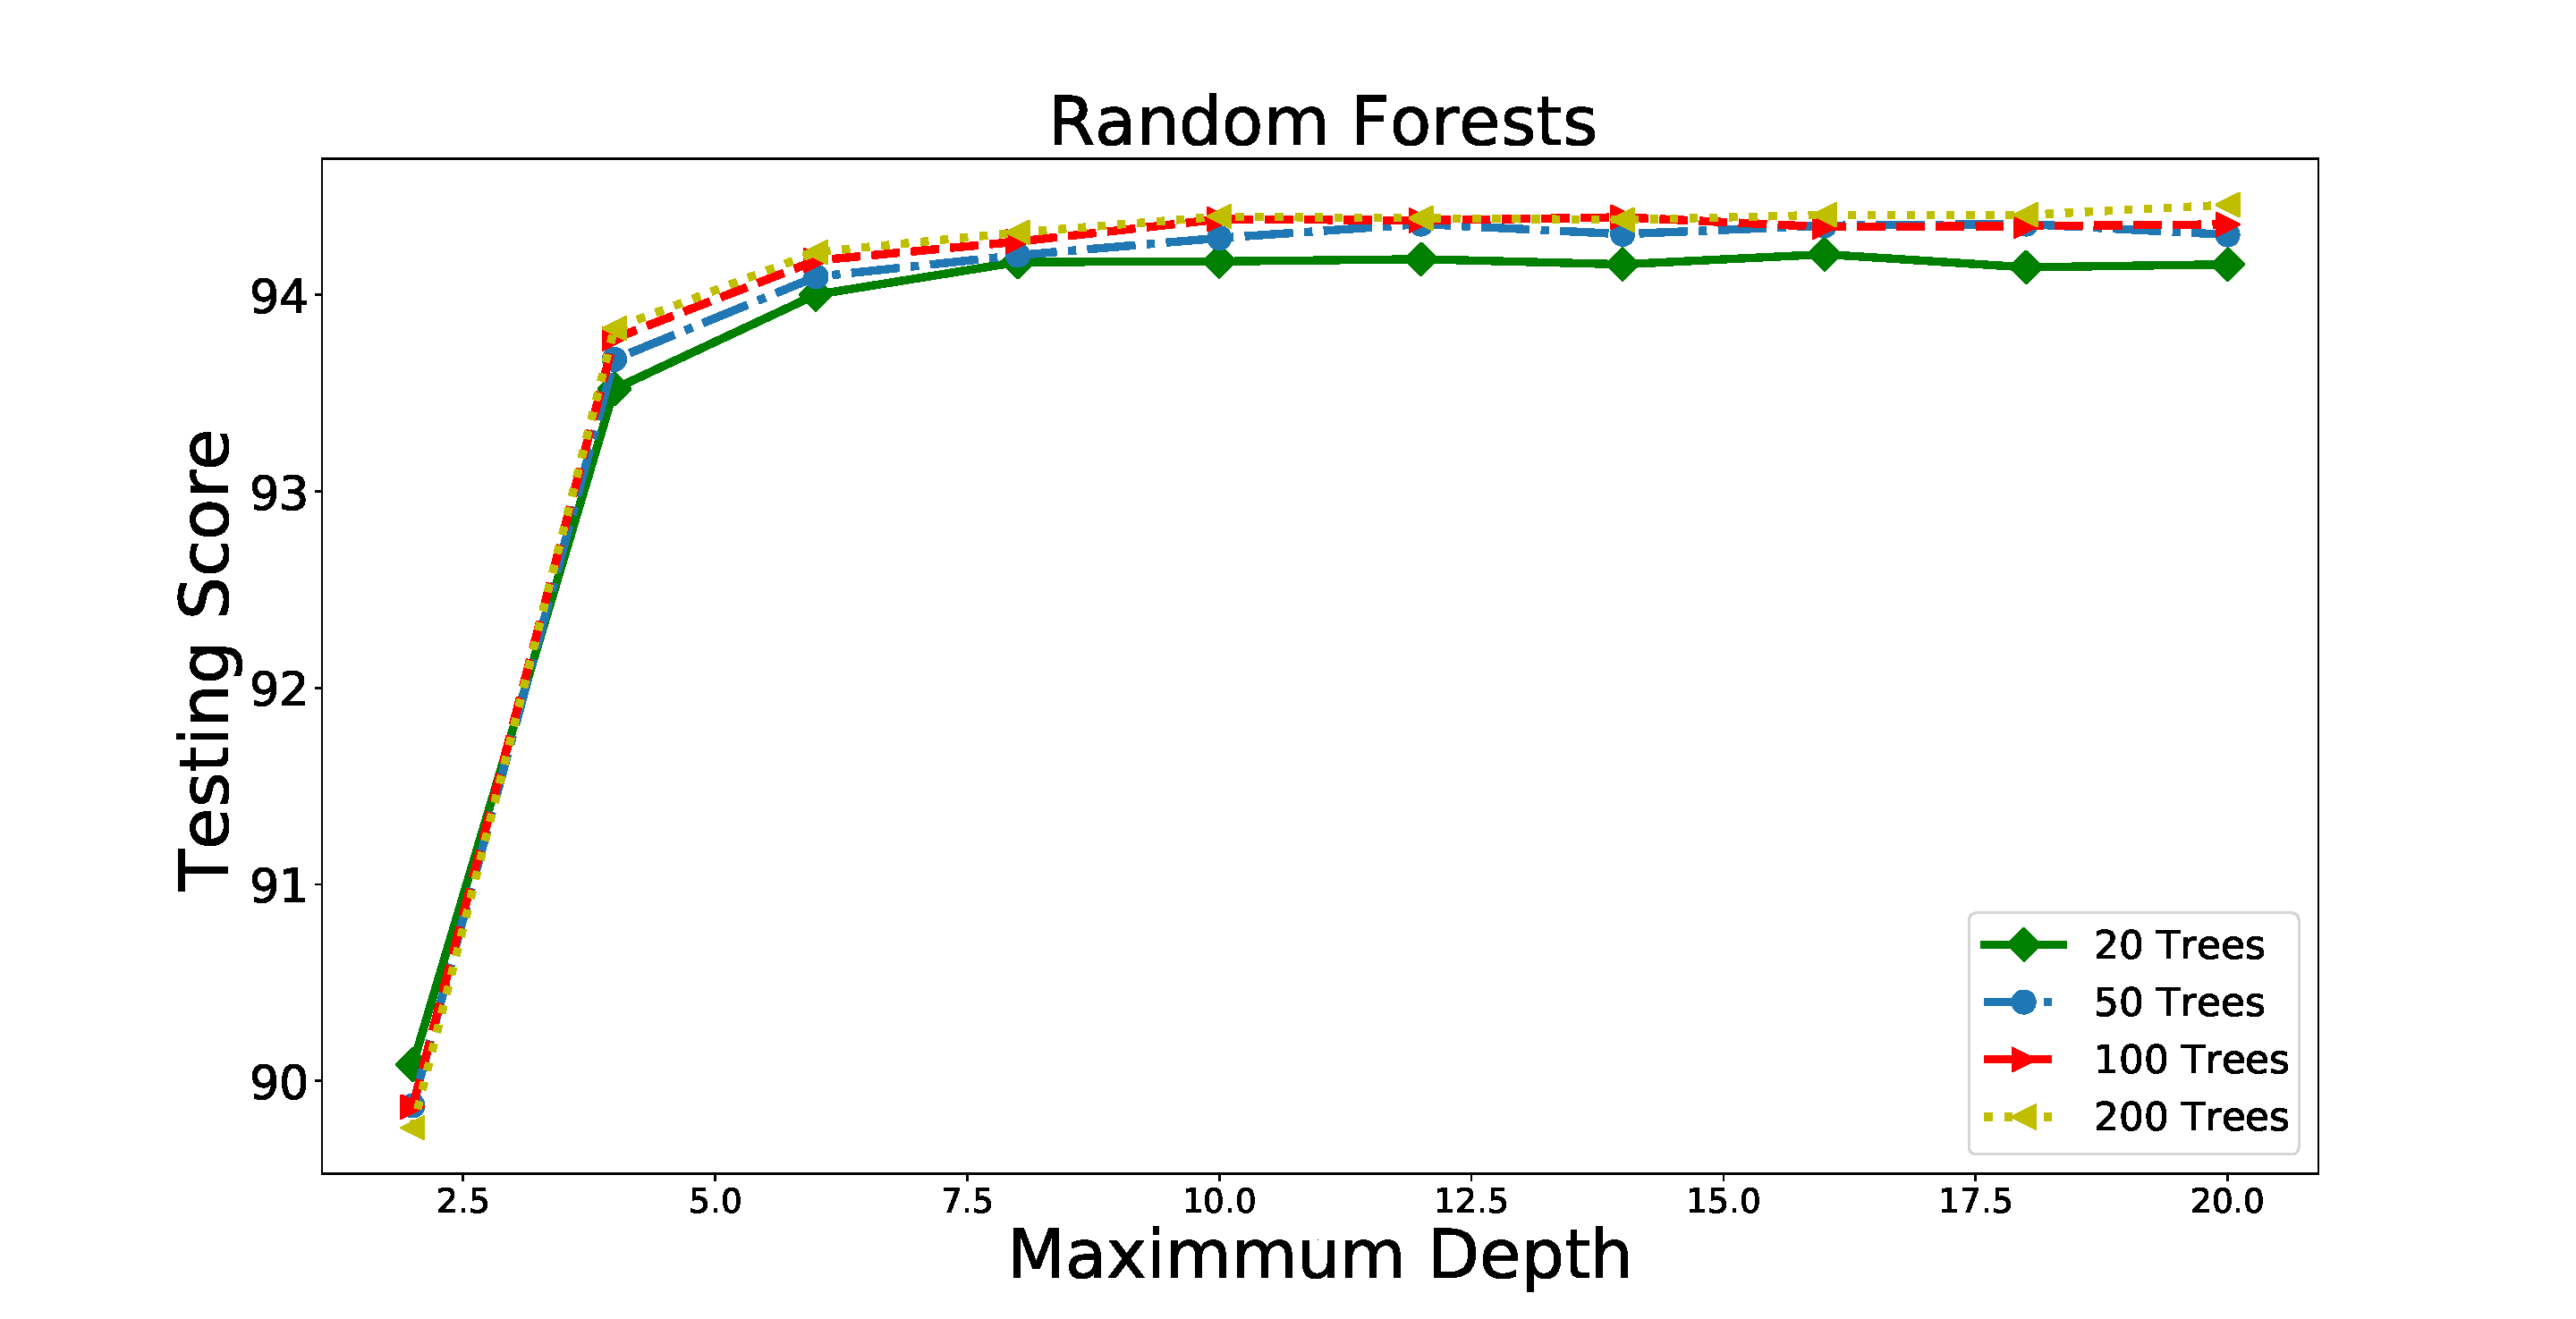
\includegraphics[width=0.5\textwidth]{plots/rf_train_multi.pdf}\\
%\hspace*{-1cm}
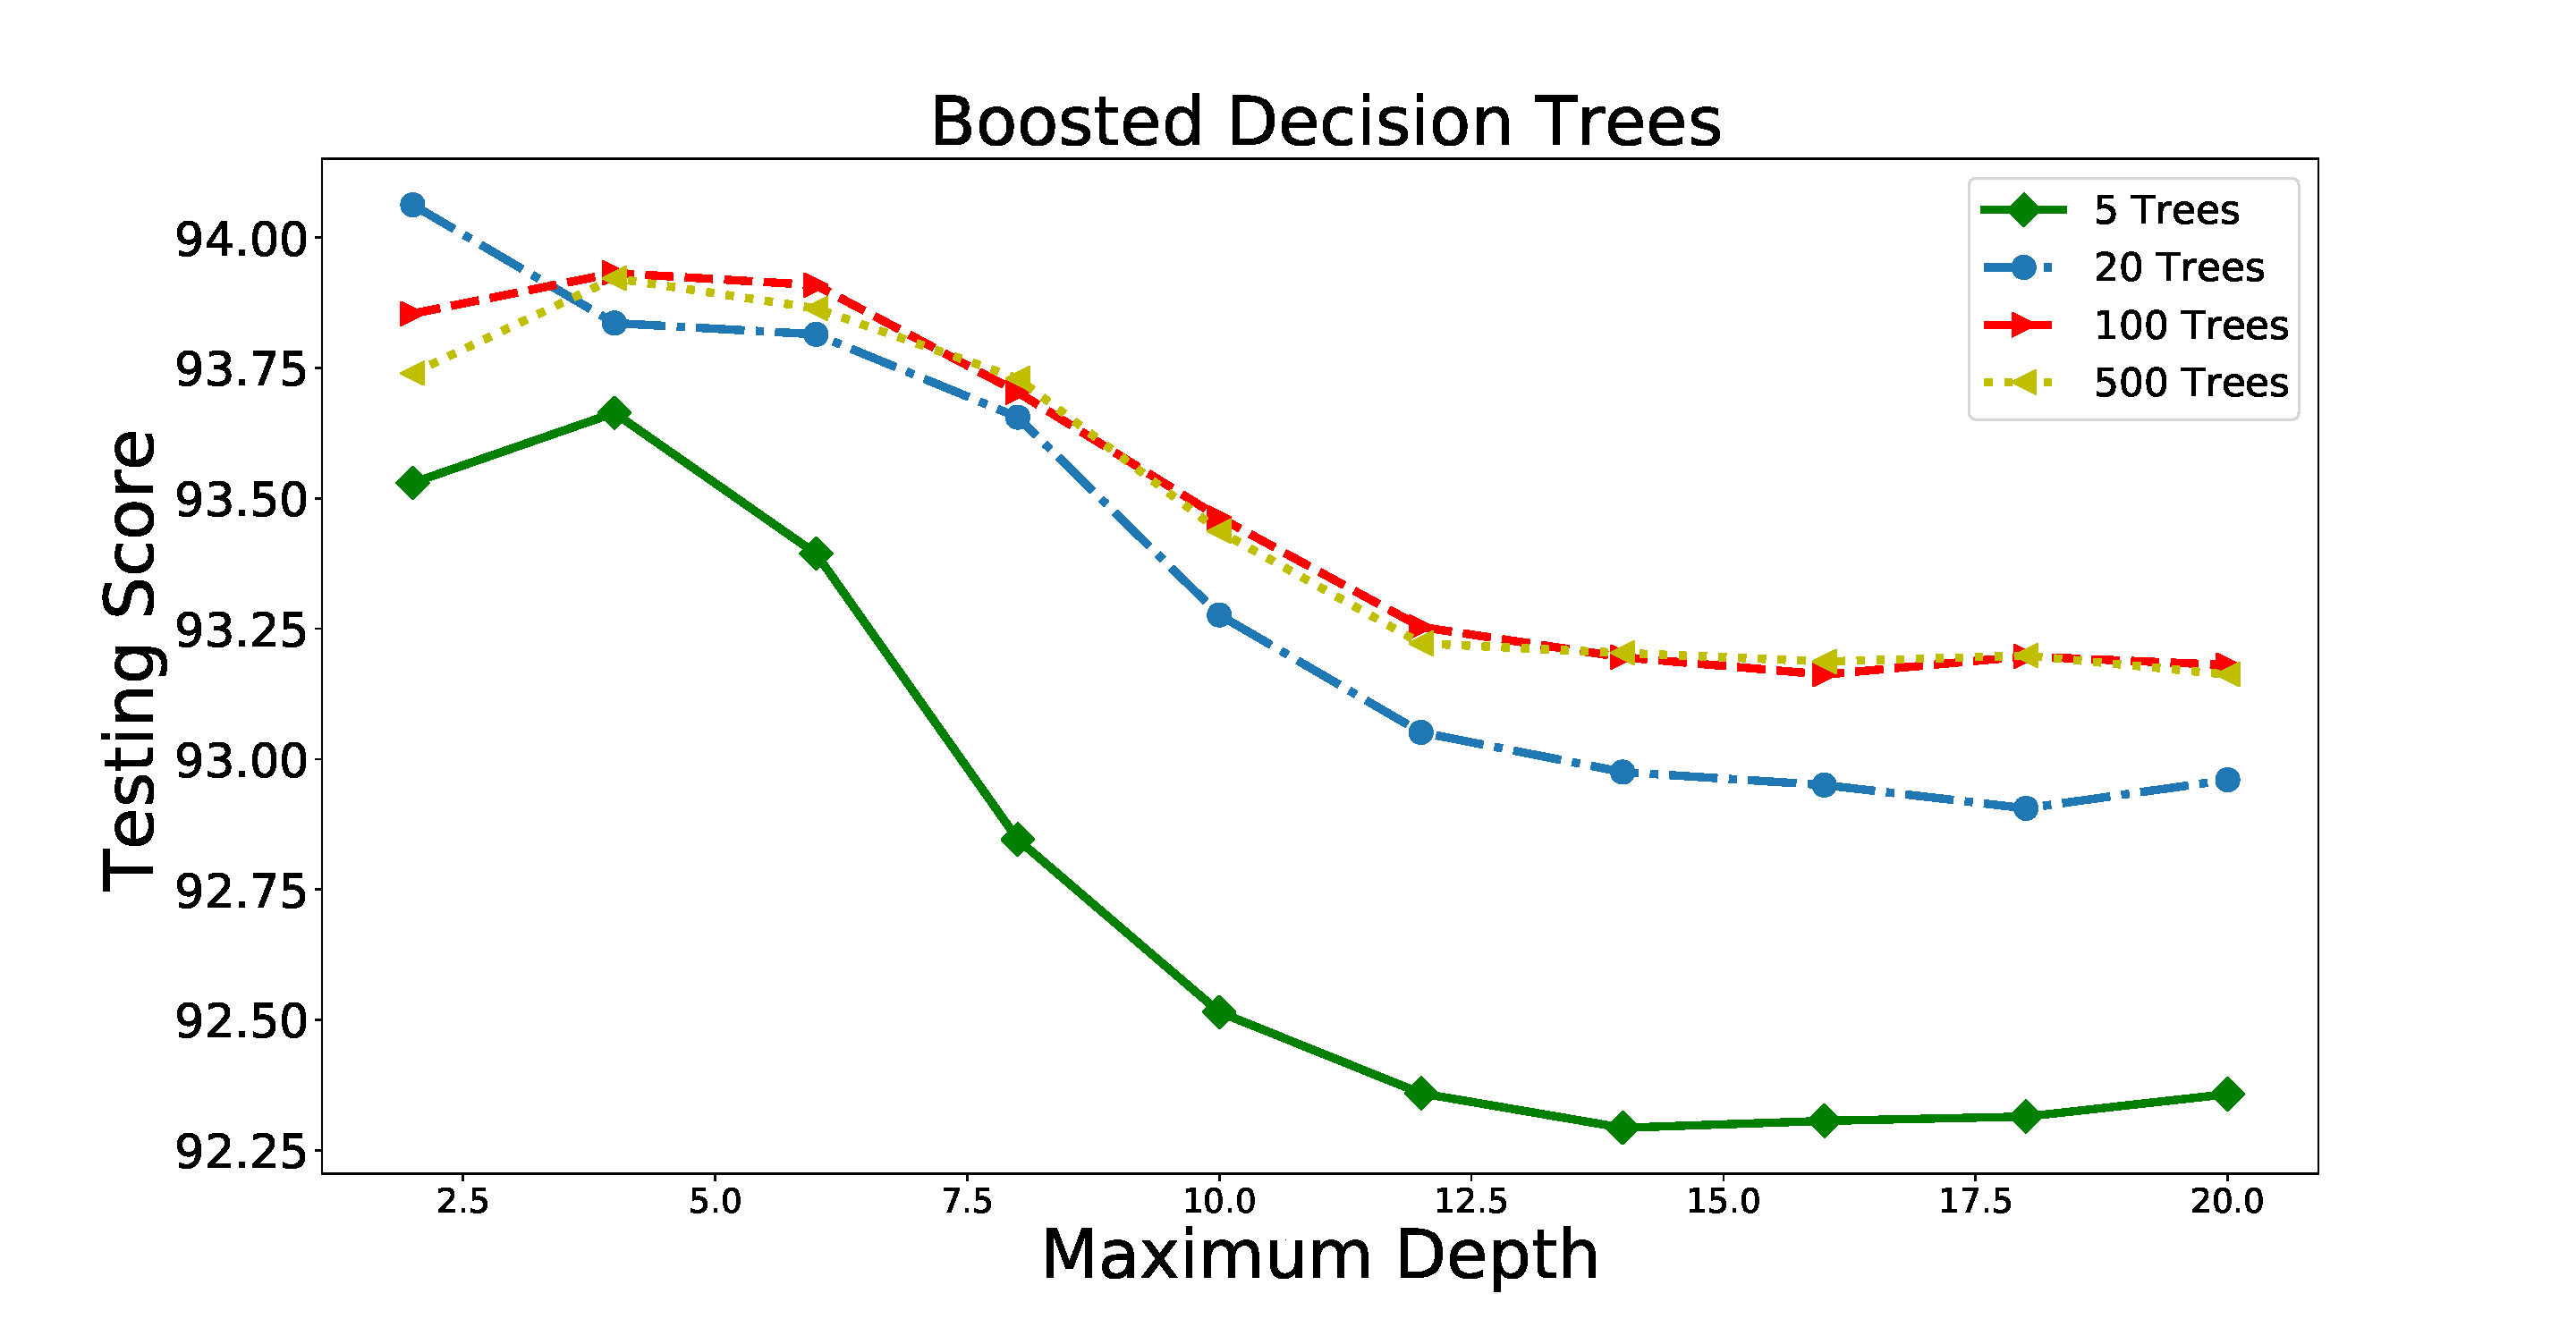
\includegraphics[width=0.5\textwidth]{plots/bdt_train_multi.pdf}
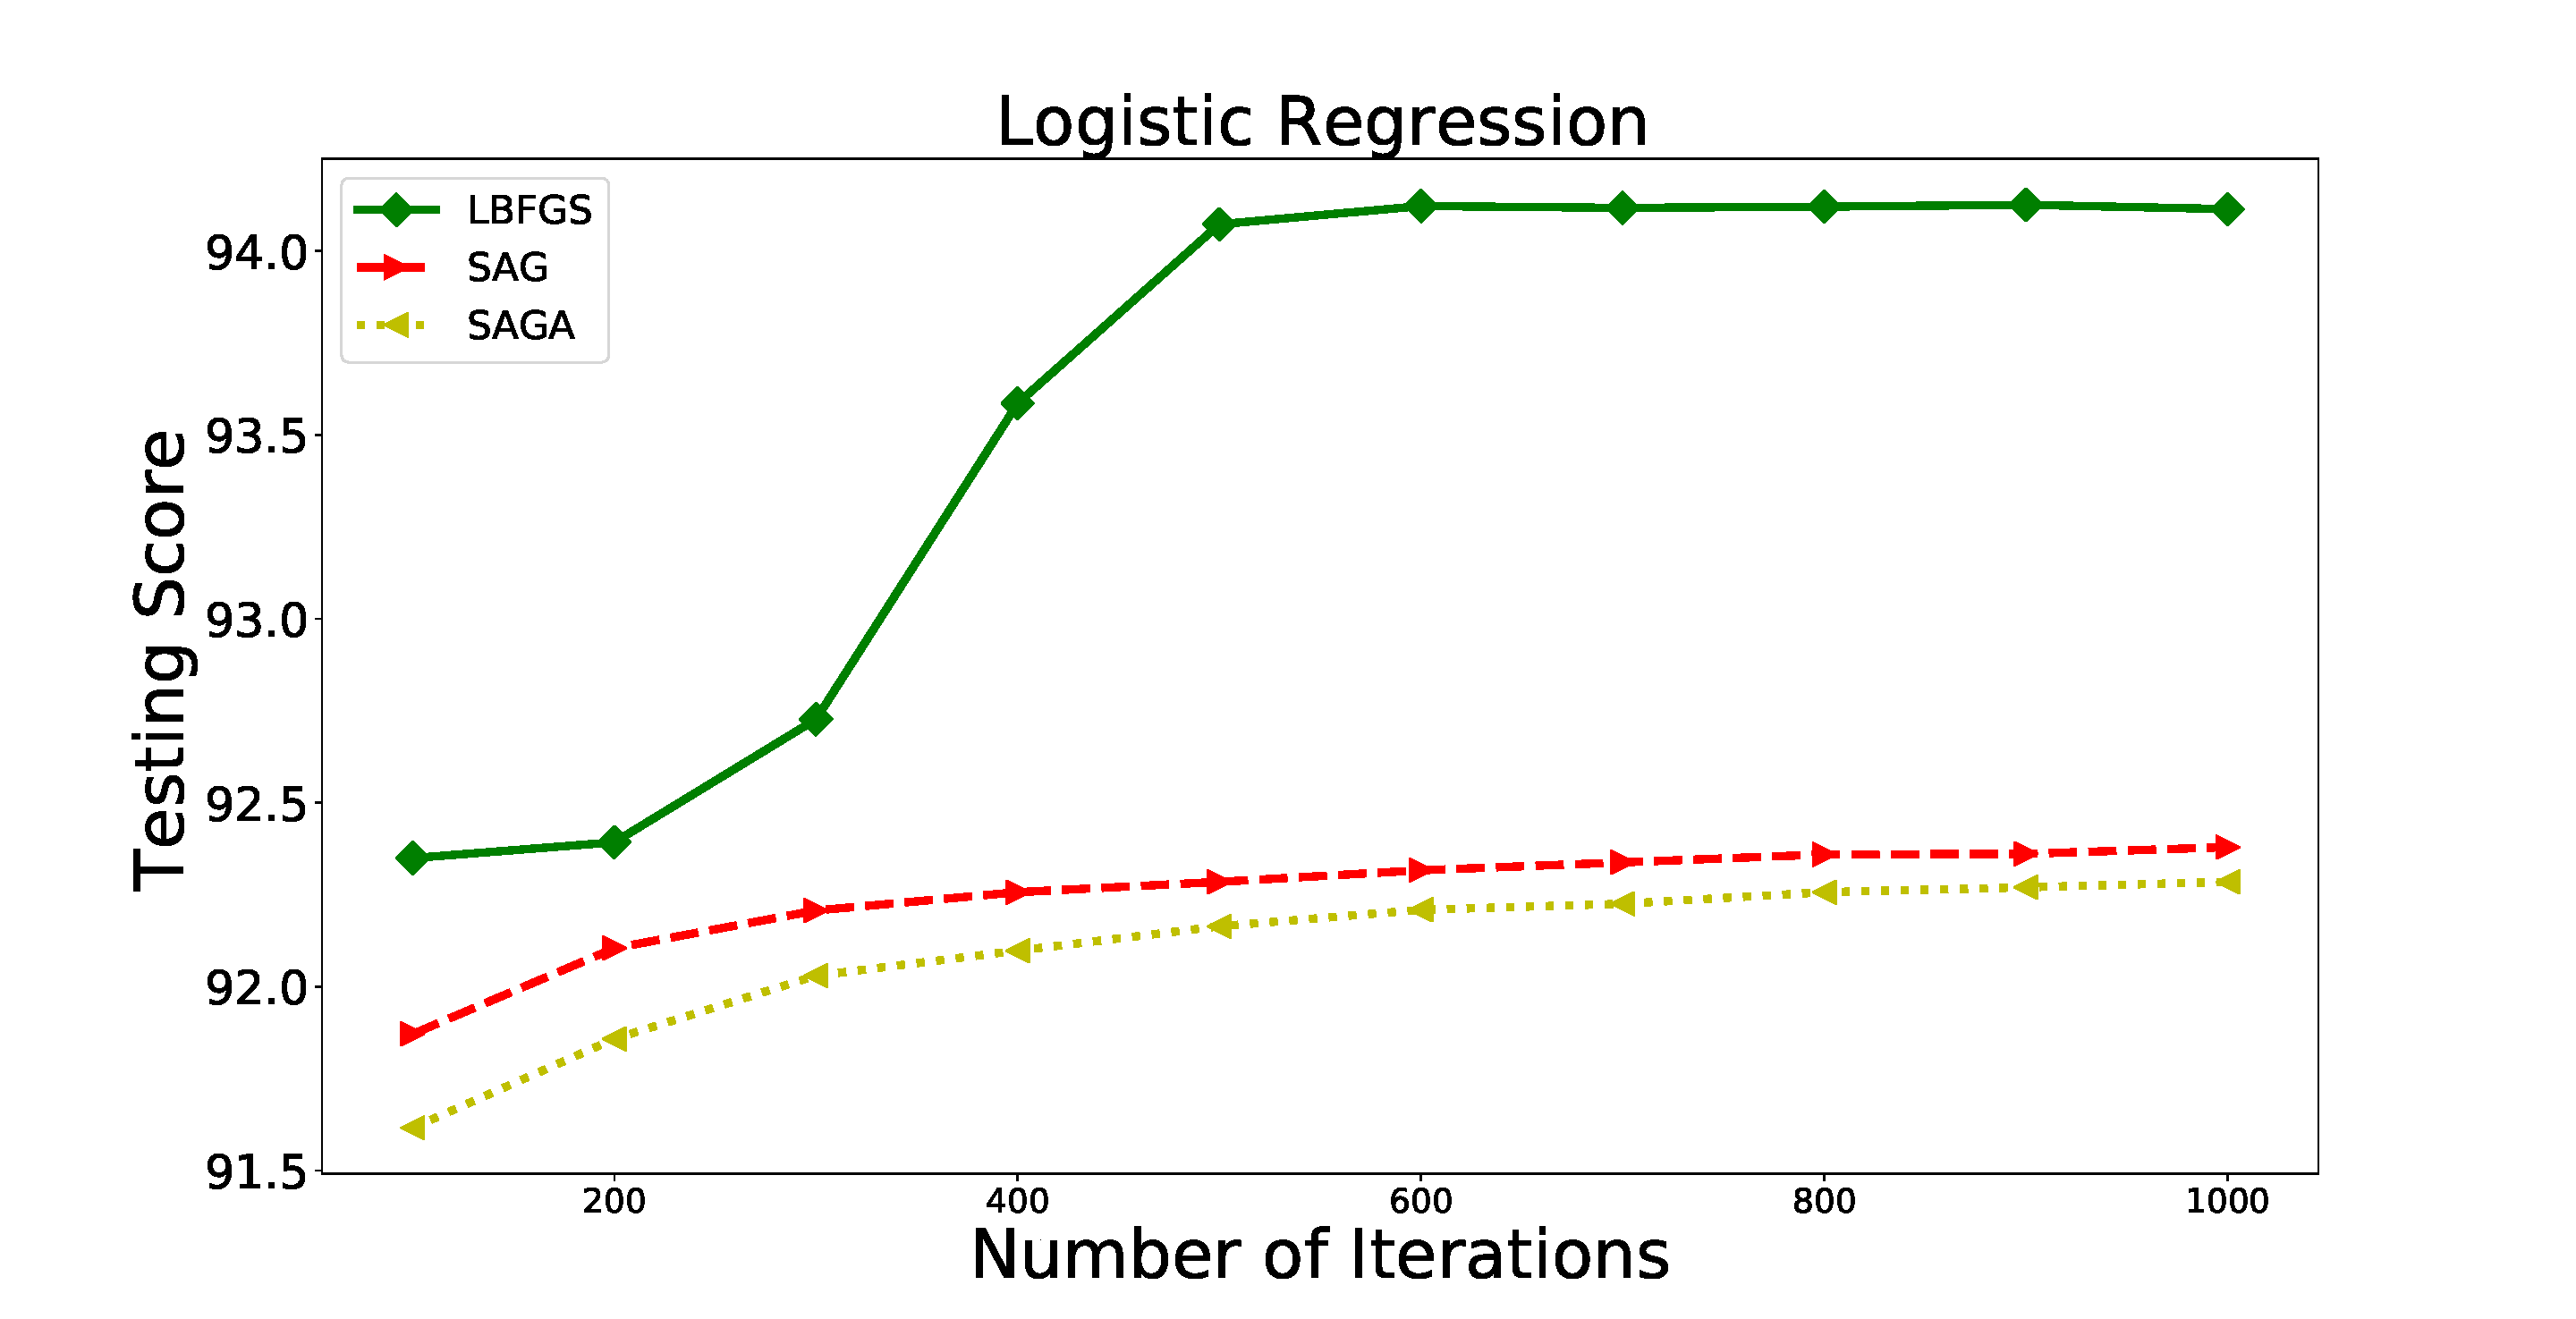
\includegraphics[width=0.5\textwidth]{plots/lr_train_multi.pdf}
\caption{Accuracy for the 3-class classification with RF, BDT and LR  methods. LR does not have liblinear solver here, since liblinear cannot handle multinomial loss.
}
\label{fig:tree_multi}
\end{figure}

\begin{figure}[h]
\center
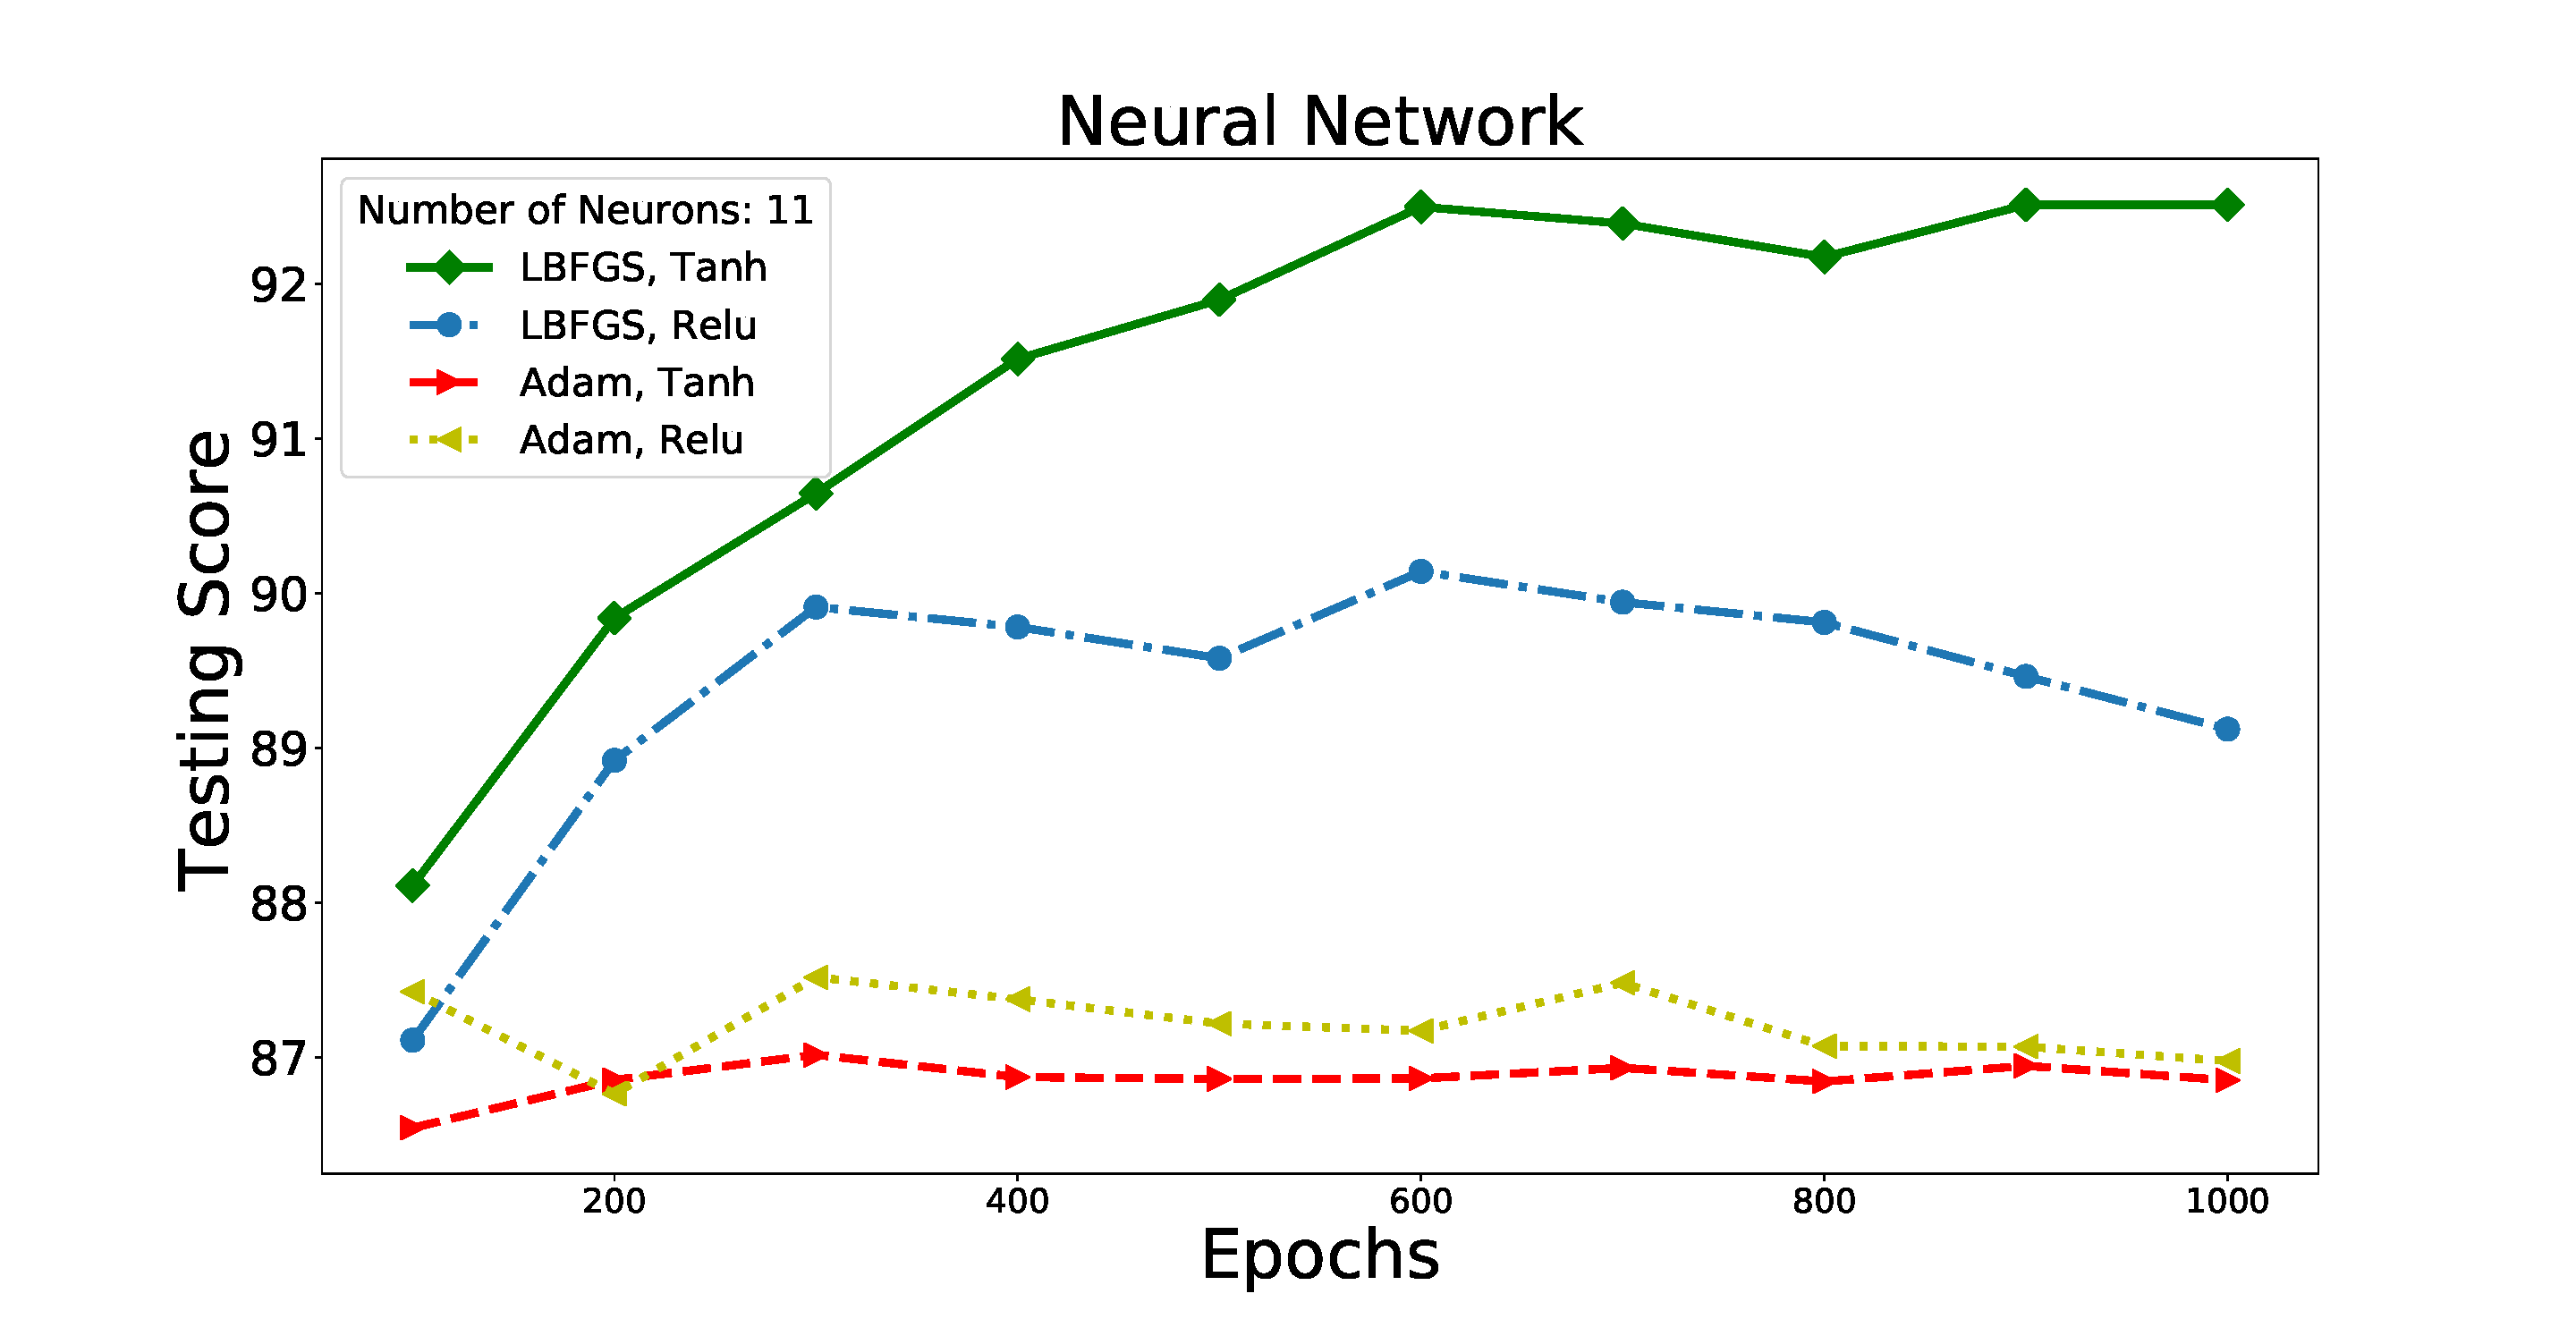
\includegraphics[width=0.5\textwidth]{plots/nn_epoch_train_multi.pdf}\\
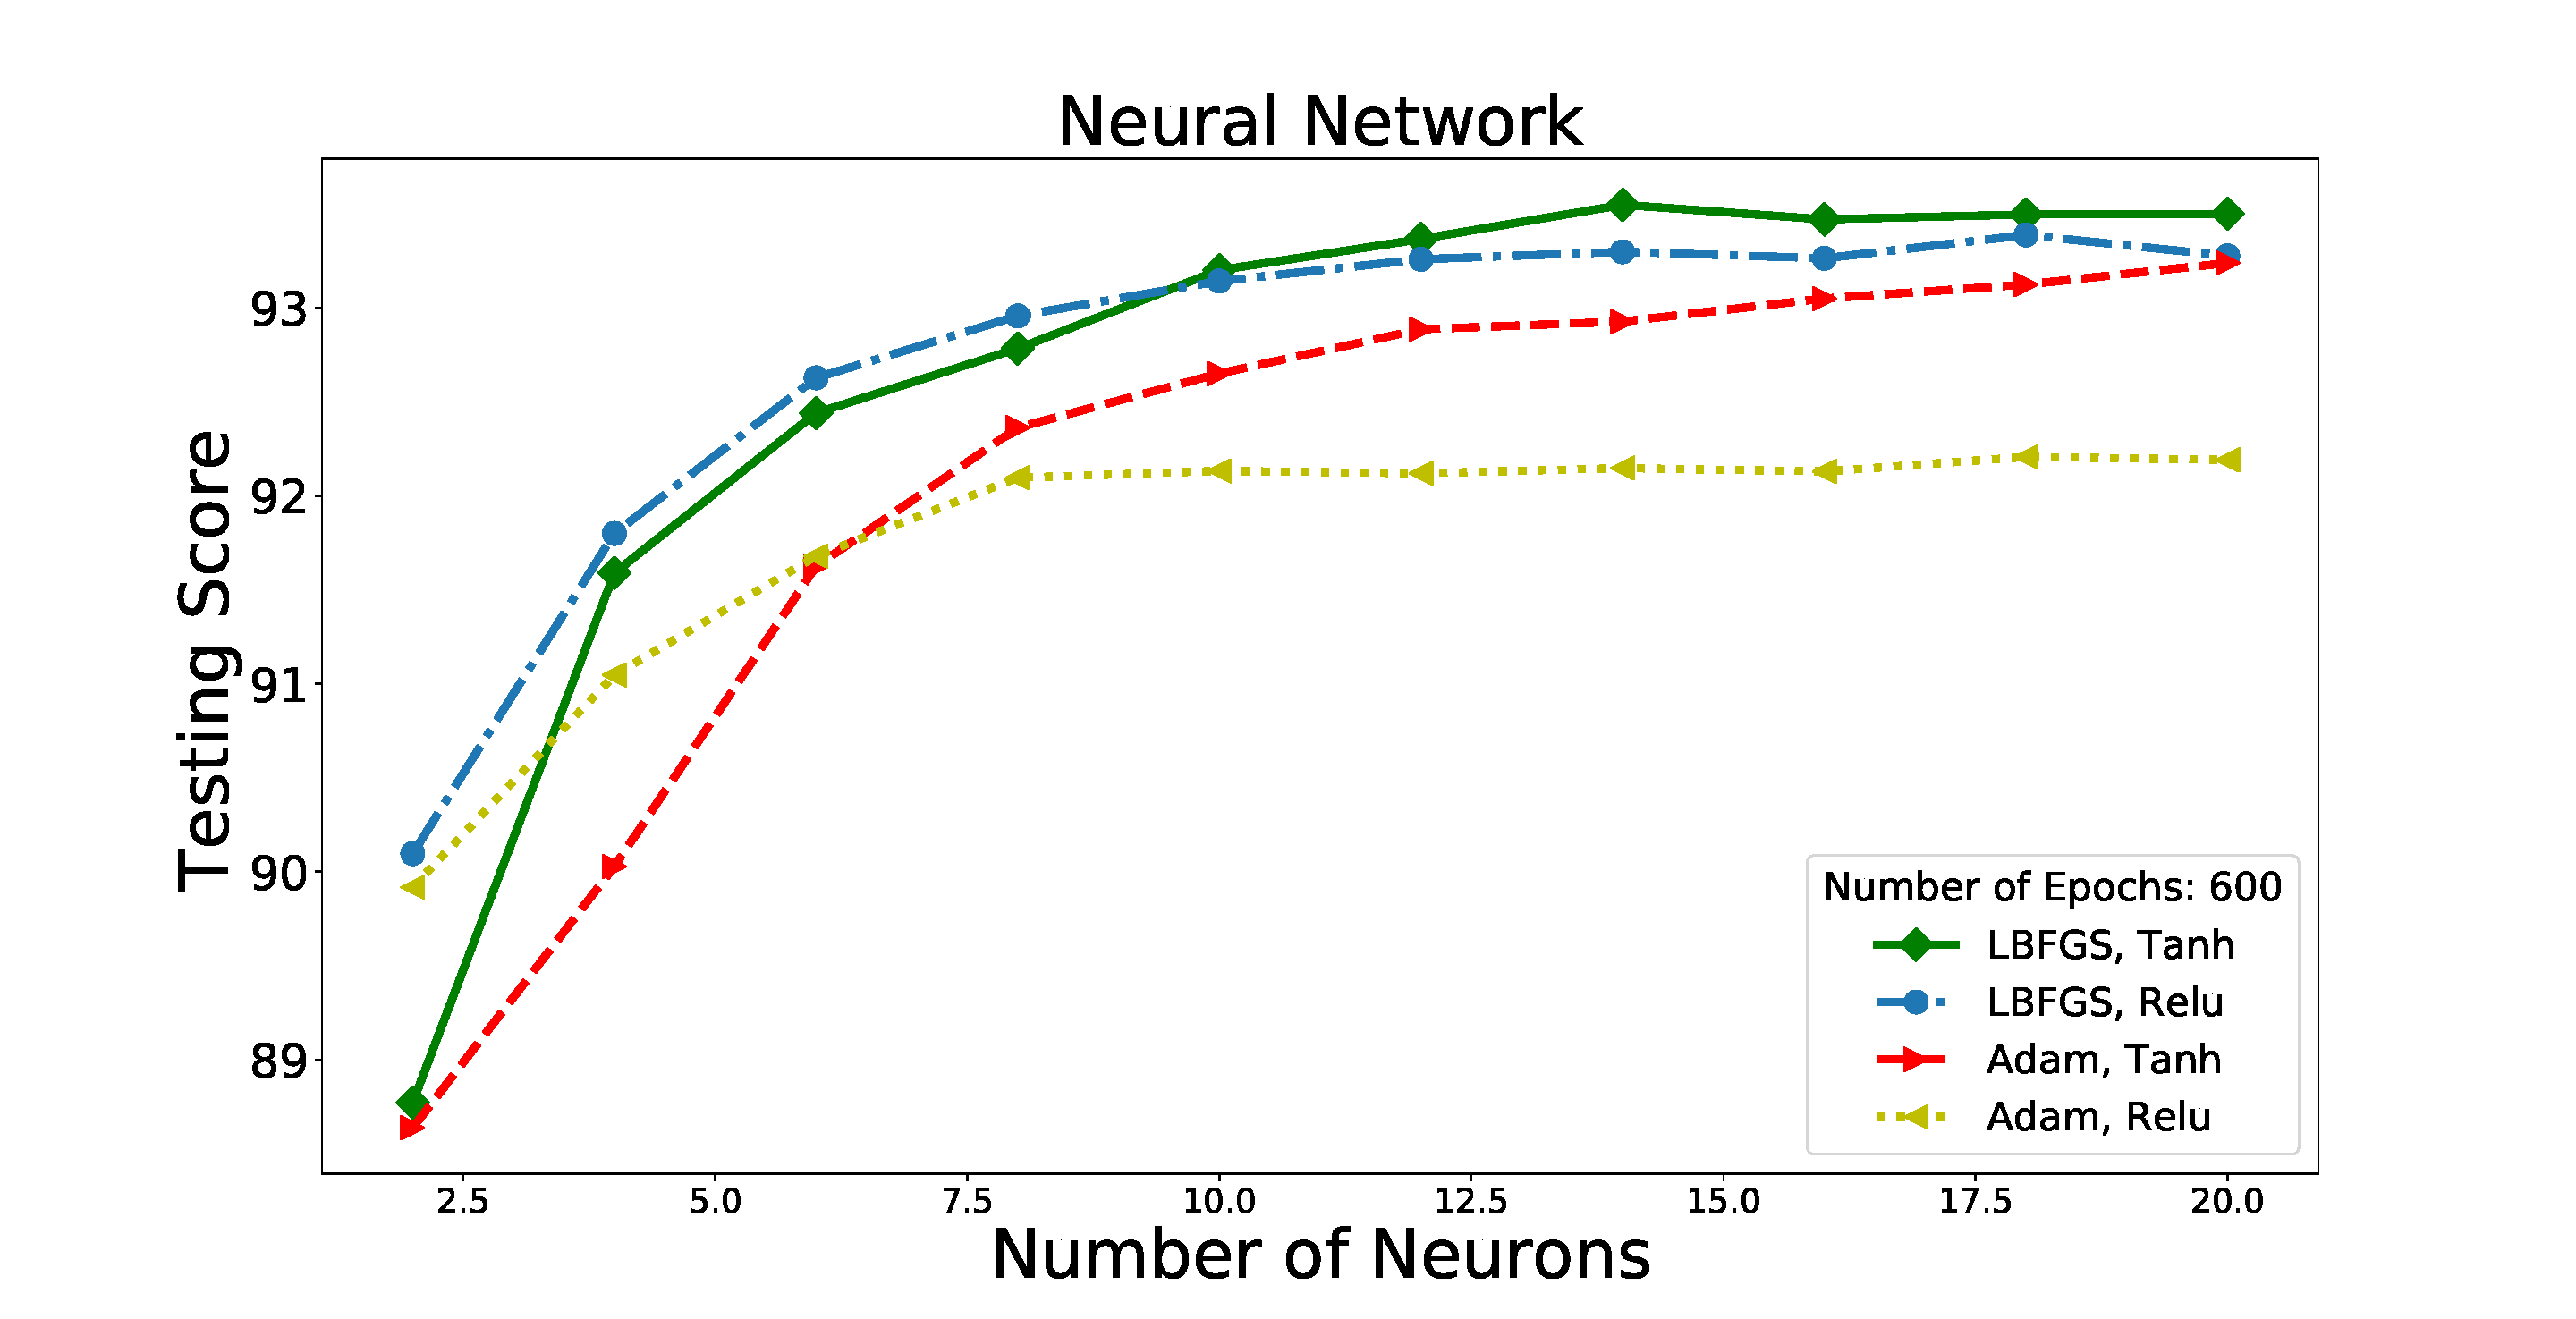
\includegraphics[width=0.5\textwidth]{plots/nn_neuron_train_multi.pdf}
\caption{Accuracy of the NN classification as a function of the number of epochs and of the number of neurons
 for the 3-class classification. 
 }
\label{fig:nets_multi}
\end{figure}


The dependence of accuracy on meta-parameters of the algorithms is shown in Figures \ref{fig:tree_multi} and \ref{fig:nets_multi}.
We see that for the tree-based algorithms, the optimal parameters are similar to the 2-class classification, i.e., 50 trees with depth 6 for RF and 100 trees with depth 2 for BDT 
provide close to optimal performance at a minimal cost in complexity (depth of the trees).
The main difference for NN and LR algorithms is that more steps are needed for convergence, especially in case of oversampling. 
In the following we use 600 epochs for NN and 500 iterations for LR instead of 300 epochs and 200 iterations respectively in the two-class case.
For NN, the accuracy stops increasing above about 10 neurons in the hidden layer (in the following we use 11 neurons for classification: the same as in the two-class case).
For oversampling, we use the oversampling factors $\sqrt{\frac{\text{\# AGN}}{\text{\# PSR}}}$ and $\sqrt{\frac{\text{\# AGN}}{\text{\# OTHER}}}$ for PSR and OTHER classes respectively (instead of $\frac{\text{\# AGN}}{\text{\# PSR}}$ and $\frac{\text{\# AGN}}{\text{\# OTHER}}$ oversampling factors in the 2-class case).
The reason for a smaller oversampling factors is to avoid overweighting the relatively small OTHER class.

\begin{figure}[h]
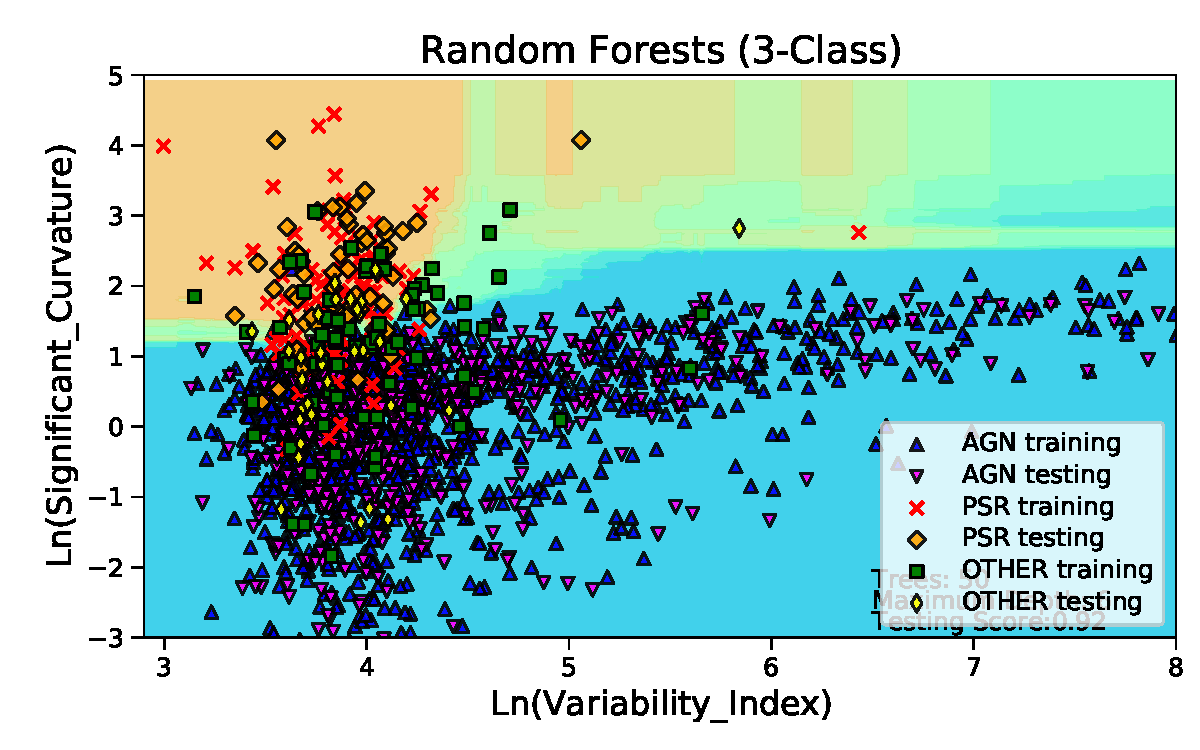
\includegraphics[width=0.46\textwidth]{plots/classification_domains/rf_50_6_3class.pdf}
\caption{Classification domains for RF in the 3-class classification.
}
\label{fig:RF_domains_3class}
\end{figure}

We show an example of domains in the 3-class case in Figure \ref{fig:RF_domains_3class}.
A class domain is determined by the class with the largest probability.
Since in the 3-class case there are two independent probabilities, which are difficult to show with a single color bar,
we present only the domains represented by three different colors: brown for PSR, green for OTHER, and blue for AGN classes.
The corresponding training and testing data are shown by red crosses and brown rotated squares for PSR, by green squares and yellow diamonds for OTHER,
and by blue and purple triangles for AGN classes.
The classification domains are averaged over 100 realizations of splitting the data into training and testing samples.
One of these splittings is shown on the figure.


The accuracies of our chosen models for classification of the 3FGL sources are presented in Table \ref{tab:selected_algs_multi}.
As in the 2-class case, the accuracies are averaged over 1000 realizations of splitting the data into training and testing samples.
We notice that accuracies presented in Table \ref{tab:selected_algs} are calculated relative to AGN and PSR classes only, if we take into account that all OTHER sources
are misclassified in this case, then the testing accuracy is reduced by about 5\% (the fraction of OTHER sources among associated sources in 3FGL),
while the accuracy of comparison with 4FGL-DR2 is reduced by about 10\% (there are 37 unassociated sources in 3FGL with OTHER class associations in 4FGL-DR2,
while there are in total 339 unassociated sources in 3FGL with associations in 4FGL-DR2).
Thus the testing accuracy of 93-94\% in Table \ref{tab:selected_algs_multi} provides at least a 1-2\% improvement over the accuracy in Table \ref{tab:selected_algs},
after taking into account the misclassification of OTHER sources in the 2-class case
and a similar improvement for the accuracy of classification of unassociated sources in 3FGL with 4FGL-DR2 associations.



\begin{table}[!h]
\hspace{-0.2cm}
\resizebox{0.47\textwidth}{!}{
    \tiny
  \centering
    \renewcommand{\tabcolsep}{0.4mm}
\renewcommand{\arraystretch}{1.6}

%\hspace{-3mm}
    \begin{tabular}{c c c c c c c}
    \hline
    \hline
    Algorithm&Parameters &  Testing\ &Std. Dev.& Comparison with \\
    & & Accuracy\ & & 4FGL-DR2 Accuracy \\
    \hline
    RF & 50 trees, max depth 6  & 93.96 & 0.85 & 85.00 \\
    RF\_O &   & 94.38 & 0.76 & 85.00 \\ 
    \hline
    BDT & 100 trees, max depth 2    &   93.72 & 0.83 & 83.24 \\
    BDT\_O &     &   93.83 & 0.80 & 85.29 \\
    \hline
    NN & 600 epochs, 11 neurons, LBFGS & 93.17 & 1.05 & 83.53 \\
    NN\_O &&  92.51 & 1.34 & 81.76 \\
    \hline
    LR & 500 iterations, LBFGS solver & 93.93 & 0.88 & 83.24 \\
    LR\_O &   & 93.01 & 0.96 & 83.24 \\
    \hline
    \end{tabular}}
    \vspace{2mm}
    \caption{Testing accuracy of the four selected algorithms for 3-class classification of 3FGL sources and comparison with associations in the 4FGL-DR2 catalog. 
    ``\_O'' denotes training with oversampling.}
    \label{tab:selected_algs_multi}
\end{table}



The 3-class classification of 4FGL-DR2 sources is performed similar to the 3-class classification of the 3FGL sources.
The differences are similar to the differences in the 2-class classification of 3FGL and 4FGL-DR2 sources:
we use 16 features (the same features as in the 2-class classification of 4FGL-DR2 sources in Section \ref{sec:4FGLprediction} but with GLON replaced by cos(GLON))
and we have 16 neurons in the hidden layer of the NN method. Furthermore, for Logistic Regression we use 1000 iterations instead of 500 as it gives better performance for oversampled cases.
The corresponding accuracies are reported in Table \ref{tab:selected_algs_4fgl_multi}.
In comparing the accuracies with the 2-class classification in Table \ref{tab:selected_algs2}, 
one has to take into account that there are 346 OTHER sources among 4116 associated sources in 4FGL-DR2, which is about 8.4\%.
Since all OTHER sources are ``misclassified'' by the 2-class classification, the 3-class classification provides an improvement of about 2-4\% compared to the 2-class classification.

\begin{table}[!h]
\hspace{-0.2cm}
%\resizebox{0.47\textwidth}{!}{
    \tiny
  \centering
    \renewcommand{\tabcolsep}{0.4mm}
\renewcommand{\arraystretch}{1.6}
    \begin{tabular}{c c c c c c}
    \hline
    \hline
    Algorithm&Parameters &  Testing&Std. Dev.\\
    & & Accuracy\ &  \\
    \hline
    RF & 50 trees, max depth 6  &92.91&0.66\\
    RF\_O &   &92.83&0.63 \\
    \hline
    BDT & 100 trees, max depth 2    &   92.51&0.67 \\
    BDT\_O &     &   92.27&0.67 \\
    \hline
    NN & 600 epochs, 16 neurons, LBFGS & 91.86&0.72\\
    NN\_O &  & 90.26&0.83\\
    \hline
    LR & 1000 iterations, LBFGS solver & 92.63&0.67 \\
    LR\_O &  &92.22&0.69\\
    \hline
     
    \end{tabular}%}
    \vspace{2mm}
    \caption{Testing accuracy of the four selected algorithms for the 3-class classification of 4FGL-DR2 sources. 
    ``\_O'' denotes training with oversampling.}
    \label{tab:selected_algs_4fgl_multi}
\end{table}


The numbers of unassociated sources classified by all 8 methods as AGNs, pulsars, and other sources for 3FGL and 4FGL-DR2 catalogs are presented in Table \ref{tab:prediction_2and3class} in the ``3-class'' rows.
For each algorithm the most probable class of the source is determined by the class with the largest probability.
Since there are three classes, the largest probability can have the value just above 1/3.
The ``Mixed'' column shows the number of sources with different classification results for different algorithms.

\begin{table}[!h]
%\resizebox{0.3\textwidth}{!}{
    %\tiny
  %\centering
 \renewcommand{\tabcolsep}{0.3mm}
\renewcommand{\arraystretch}{1.5}

    \begin{tabular}{l c c c c}
    \hline
    \hline
    4FGL-DR2 class & \multicolumn{4}{c}{3FGL prediction} \\
      &\ AGN &\ PSR &\ OTHER &\ MIXED \\
    \hline
    AGN & 238 & 2 &  1 & 17 \\ % 258
    PSR & 12 & 17 &  0 & 16 \\ % 45
    OTHER & 6 & 5 & 8 & 18 \\ % 37
    \hline
    \end{tabular}%}
    \vspace{0.2cm}
    \caption{Comparison of classes predicted for unassociated sources in the 3FGL catalog using 3-class classification
    with associations in the 4FGL-DR2 catalog. 
}
    \label{tab:3FGL_vs_4FGL_2class}
\end{table}


Classification of \Fermi-LAT 4FGL sources into three classes was considered earlier by, e.g., \cite{2021RAA....21...15Z}.
\cite{2021RAA....21...15Z} have primarily used a two-step classification procedure, where in the first step AGNs are separated from the rest of sources and in the second step the remaining sources are split into pulsars and other sources.
\cite{2021RAA....21...15Z} have also tested a simultaneous classification of sources into three classes (AGN, pulsars, other),
but the results were inconsistent for the two ML algorithms used by \cite{2021RAA....21...15Z} (RF and NN).
In particular, the number of OTHER sources predicted by NN was zero.
In our case, the predictions of various algorithms are relatively consistent with each other.
For example, in the 3FGL (4FGL-DR2) catalog all 8 methods classify 69 (271) unassociated sources as OTHER.
Also, 8 out of 37 unassociated 3FGL sources, which are associated to OTHER sources in 4FGL-DR2, are classified by all 8 algorithms as
OTHER (6 are classified as AGNs, 5 as PSRs, and 18 have mixed classification).

We also used the 3-class classification for a candidate list of most promising objects. We summed up the probabilities of all 8 methods for the three classes and chose the threshold of 7.0 for the column $\text{OTHER\_TOTAL}$. This is a stringent condition on the probability that a source belongs to the other class. Furthermore, we sub-selected the unassociated candidates in 4FGL-DR2 and have created our final candidate list of 30 sources based on 4FGL-DR2 features, shown in table \ref{tab:allotherspredicted}.
\pgfplotstableread[col sep=comma]{tables/4FGLDR2_Candidates_OTHER.csv}\loadedtable
\begin{table}
\hspace{-0.5cm}
\tiny
\pgfplotstabletypeset[columns={Source_Name_4FGL,GLON,GLAT,OTHER_TOTAL,Category_Prob_3FGL},
column type=l,
string type,
every head row/.style={before row={\hline \hline},after row=\hline,},
every last row/.style={after row=\hline},
columns/Source_Name_4FGL/.style={column name=Source\_Name\_4FGL},
columns/GLON/.style={column name=GLON,numeric type,fixed,precision=2},
columns/GLAT/.style={column name=GLAT,numeric type,fixed,precision=2},
columns/OTHER_TOTAL/.style={column name=Sum(Prob),numeric type,fixed,precision=2},
columns/Category_Prob_3FGL/.style={column name=Cat.(3FGL)},
]\loadedtable
\normalsize
\caption{\label{tab:allotherspredicted}
List of unassociated 4FGL DR2 sources predicted to be OTHER class. These are all predicted to be 'OTHER' sources by all 8 algorithms. We also attach the category from 3FGL data where the association is available. Sum(Prob) is the total sum of the OTHER class probabilities.}
\end{table}

The maximum probability is $7.48\pm0.14$ for the source 4FGLJ1800.2-2403c. Out of these 30 sources only two have 0 flags in 4FGL, and only 8 have an association with the previous FGL catalogs (column name ASSOC\_FGL). Furthermore, we tried to find whether recent work could be found for some of these sources and used the Simbad database for this purpose. Out of the sources with Simbad entries the following 8 sources had extra associations (ordered according to probability of being OTHER source):
\begin{enumerate}
\item 4FGL J1800.2-2403c. The source with the greatest probability has no entry in Simbad. However, it is associated with the 1FGL source 1FGL J1800.5-2359c, which is also associated with the associated OTHER source 4FGL J1800.7-2355 of unk class and is in the region of the SNR W28 \citep{2020MNRAS.495.2909R}.
\item 4FGL J1842.7-0326: Associated with 3FGL J1843.7-0322 and found near the HESS source HESS J1843-033, next to the SNR G28.6-0.1 \citep{2018A&A...612A...1H}. This source was also the 67th source amongs 120 unassociated sources according to significance (>10) in the list of \citet{2016ApJ...820....8S} where the RF and LR methods predicted it to be a young pulsar based on the 2-class classification. In our 3FGL multi-class catalog, this source has a 'MIXED' prediction.
\item 4FGL J1626.0-4917c: In 3FGL as 3FGL J1626.2-4911. Part of the third Fermi catalog of hard sources as 3FHLJ1626.3-4915 \citep{2017ApJS..232...18A}. Associated with HESS J1626-490. It was also part of the 27 sources shortlisted by \citet{2020MNRAS.495.1093H} who used a machine learning technique to select sources for analysis from the 3FHL. Also has an 'OTHER' prediction based on 3FGL values.
\item 4FGL J1849.4-0117: In 3FGL as 3FGL J1849.5-0124c. In the region of Galactic mini starburst W43 studied by \citet{2020A&A...640A..60Y}. Has a 'MIXED' prediction for 3FGL values.
\item 4FGL J1109.4-6115e. In 3FGL as 3FGLJ1111.9-6038. Associated with the extended galactic source FGES J1109.4-6115 \citep{2017ApJ...843..139A}. Near the speculated SFR 4FGL J1115.1-6118 in there region of  Young Massive Stellar Cluster NGC 3603 \citep{2020ApJ...897..131S}. 'MIXED' prediction with 3FGL values.
\item 4FGL J1850.2-0201: Also in the region of the starburst W43 \citep{2020A&A...640A..60Y}.
\item 4FGL J1801.8-2358: Associated with HESS J1800-240A and 2FHL J1801.7-2358. Located south of the SNR W28 \citep{2020MNRAS.495.2909R}.
\item 4FGL J1855.8+0150: In the region of SNR W44 \citep{2020ApJ...896L..23P}.
\end{enumerate}
Sources which had another Simbad object within 1 arcminute of them are shown in table \ref{tab:otherspredicted}, where we list the total probability and the type of object near the 4FGL source.
\pgfplotstableread[col sep=comma]{tables/4FGLDR2_OTHER_SIMBAD.csv}\loadedtable
\begin{table}
\hspace{-0.5cm}
\tiny
\pgfplotstabletypeset[columns={Source_Name_4FGL,OTHER_TOTAL,main_type,Sep(arksec)},
column type=l,
string type,
every head row/.style={before row={\hline \hline},after row=\hline,},
every last row/.style={after row=\hline},
columns/Source_Name_4FGL/.style={column name=Source\_Name\_4FGL},
columns/OTHER_TOTAL/.style={column name=Sum(Prob),numeric type,fixed,precision=2},
columns/main_type/.style={column name=SIMBAD\_Type},
columns/Sep(arksec)/.style={column name=Sep (arcsec),numeric type,fixed,precision=1}
]\loadedtable
\normalsize
\caption{\label{tab:otherspredicted}
Connection of unassociated 4FGL-DR2 sources predicted to be OTHER with Simbad database within 1 arc minute of the sources. We list only sources which have a seperate match than their 4FGL or 3FGL name. Abbreviations: YSO = Young Stellar Object, AGB = Asymptotic Giant Branch Star, MolCld = Molecular Cloud, DkNeb =Dark Cloud (nebula). }
\end{table}
We have saved this candidate list with the rest of the catalogs. Furthermore, there are 6 PSR candidates in our multi-class classification with a probability sum $\text{PSR\_TOTAL}> 7.0$. These are shown in table \ref{tab:psrpredicted}. All of these sources are also predicted to be pulsars as part of our 29 PSR sources mentioned in section 4 (using both 4FGL and 3FGL features). 2 of these are also present in the Parkes survey mentioned before. Interestingly. none of these sources have a sum of probability greater than 7 when 3FGL features are used, but 5 of them are categorized as PSRs in 3FGL.
\pgfplotstableread[col sep=comma]{tables/4FGLDR2_PSR.csv}\loadedtable
\begin{table}
\hspace{-0.1cm}
\tiny
\pgfplotstabletypeset[columns={Source_Name_4FGL,GLON,GLAT,PSR_TOTAL_4FGL,PSR_TOTAL_3FGL,Category_Prob},
column type=l,
string type,
every head row/.style={before row={\hline \hline},after row=\hline,},
every last row/.style={after row=\hline},
columns/Source_Name_4FGL/.style={column name=Source\_Name\_4FGL},
columns/GLON/.style={column name=GLON,numeric type,fixed,precision=2},
columns/GLAT/.style={column name=GLAT,numeric type,fixed,precision=2},
columns/PSR_TOTAL_4FGL/.style={column name=SP1,numeric type,fixed,precision=2},
columns/PSR_TOTAL_3FGL/.style={column name=SP2,numeric type,fixed,precision=2},
columns/Category_Prob/.style={column name=Cat.(3FGL)},
]\loadedtable
\normalsize
\caption{\label{tab:psrpredicted}
Unassociated 4FGL-DR2 sources predicted to be PSR by the multi class prediction. All of these sources have a corresponding 3FGL association. SP1 and SP2 here represent the sum of PSR class probabilities for 4FGL-DR2 and 3FGL respectively.}
\end{table}



\section{Application of probabilistic catalogs for population studies}
\lb{sec:pop_studies}

\subsection{Number of sources as a function of flux}
\lb{sec:dNdS}


In this section we show how probabilistic catalogs can be used, for instance, for population studies.
One of the most important questions in gamma-ray astronomy is contribution of point sources, 
e.g., AGNs, to the extragalactic gamma-ray flux 
\citep[e.g.,][]{2010ApJ...720..435A, 2011ApJ...738..181M, 2016PhRvL.116o1105A, 2016ApJS..225...18Z, 2016ApJ...826L..31Z, 2016ApJ...832..117L, 2018ApJ...856..106D}:
if most of the extra-galactic emission is explained by point sources, then one can put stringent constraints, 
e.g., on  dark matter annihilation or decay into gamma rays 
\citep{2015ApJ...800L..27A, 2015PhRvD..91l3001D, 2015JCAP...09..008F, 2015PhR...598....1F, 2017ChPhC..41d5104L} or 
on evaporation of primordial black holes \citep{2010PhRvD..81j4019C}.
In particular, it is important to understand the contribution to the population of AGNs from the unassociated sources.
A probabilistic catalog provides an answer to the question: how many sources among the unassociated ones are expected to belong to different classes, such as pulsars or AGNs. 
One can calculate the total expected number of AGNs or pulsars among the unassociated sources, or calculate the contribution as a function of one or more parameters.
In this section we determine the numbers of AGNs and pulsars as a function of their flux.



\begin{figure*}[h]
\center
%\hspace*{-1cm}
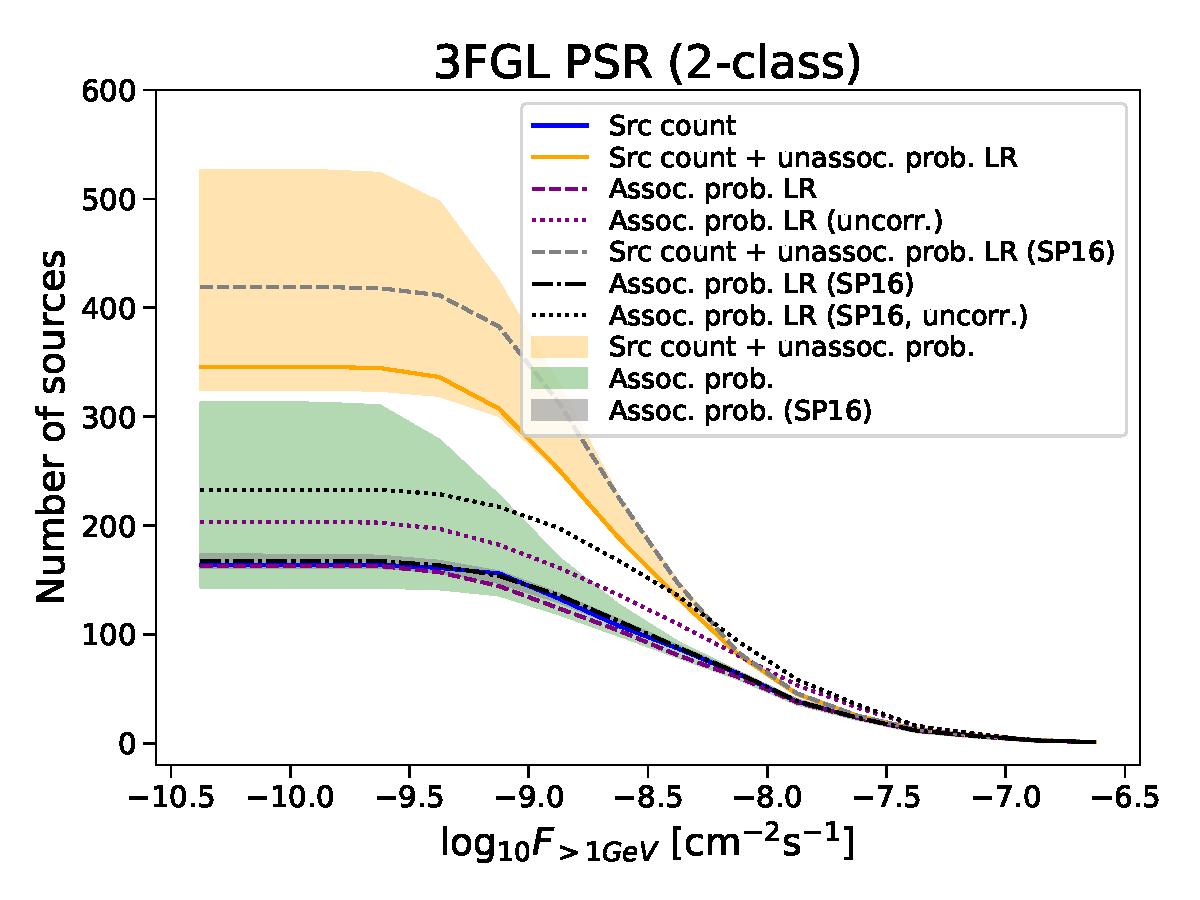
\includegraphics[width=0.45\textwidth]{plots/N_logS_3FGL_PSR_SazP_add_os.pdf}
%\hspace*{-1cm}
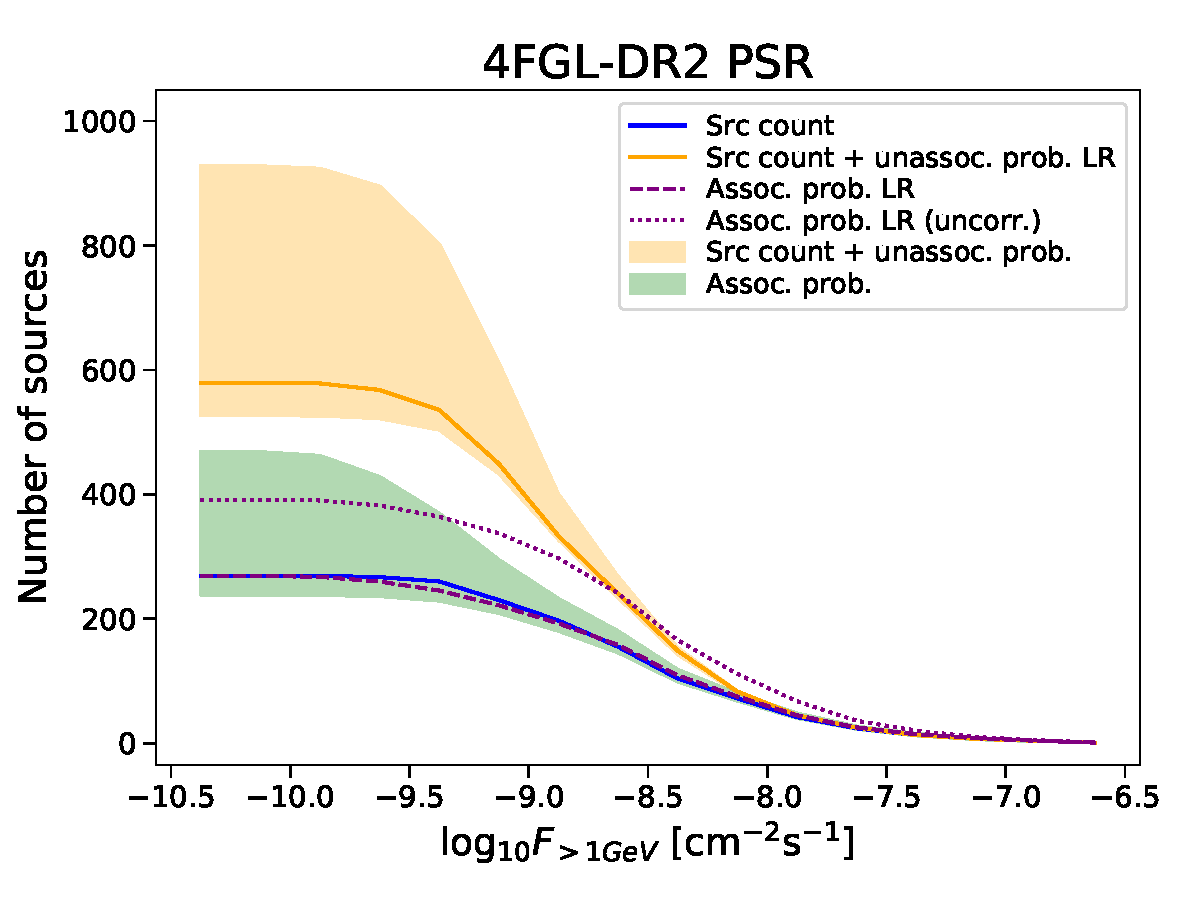
\includegraphics[width=0.45\textwidth]{plots/N_logS_4FGL-DR2_PSR_add_os.pdf} \\
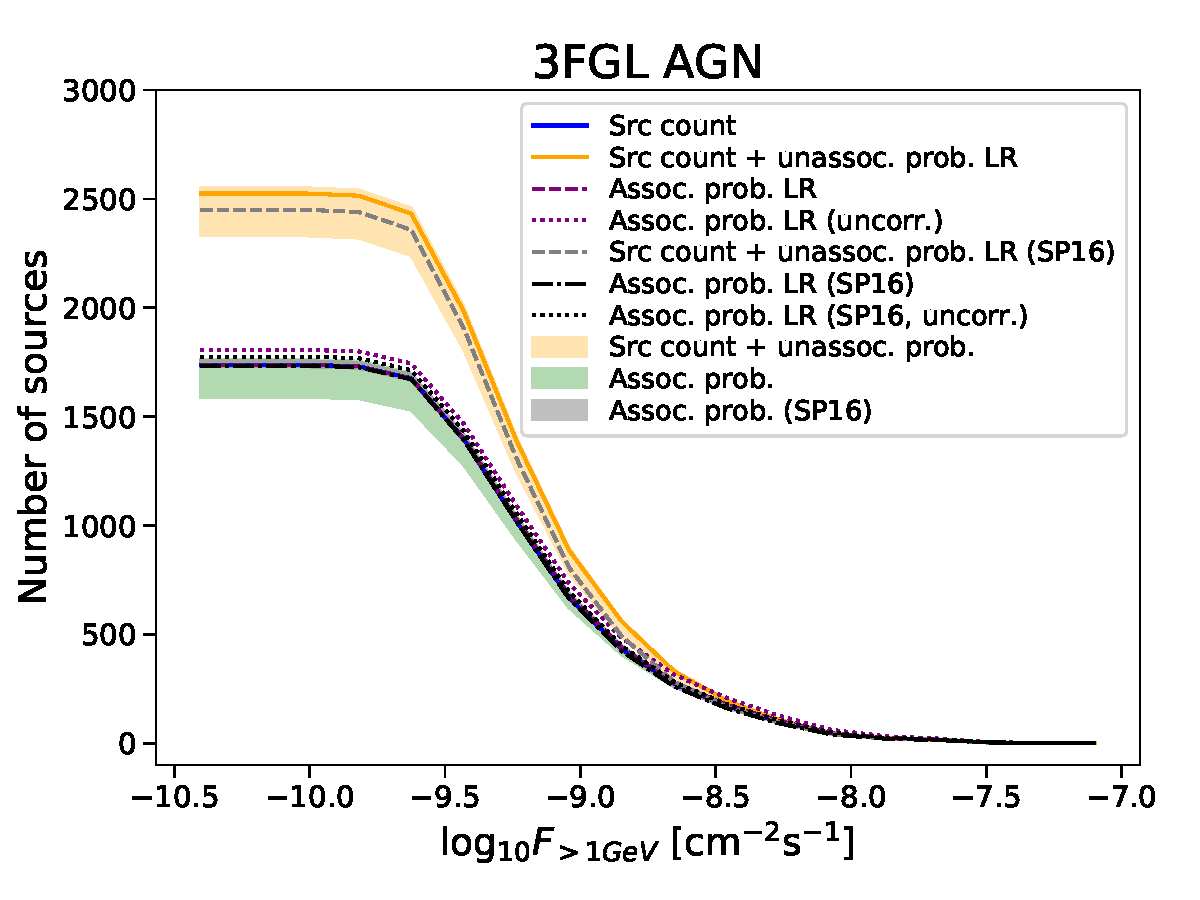
\includegraphics[width=0.45\textwidth]{plots/N_logS_3FGL_AGN_SazP_add_os.pdf}
%\hspace*{-1cm}
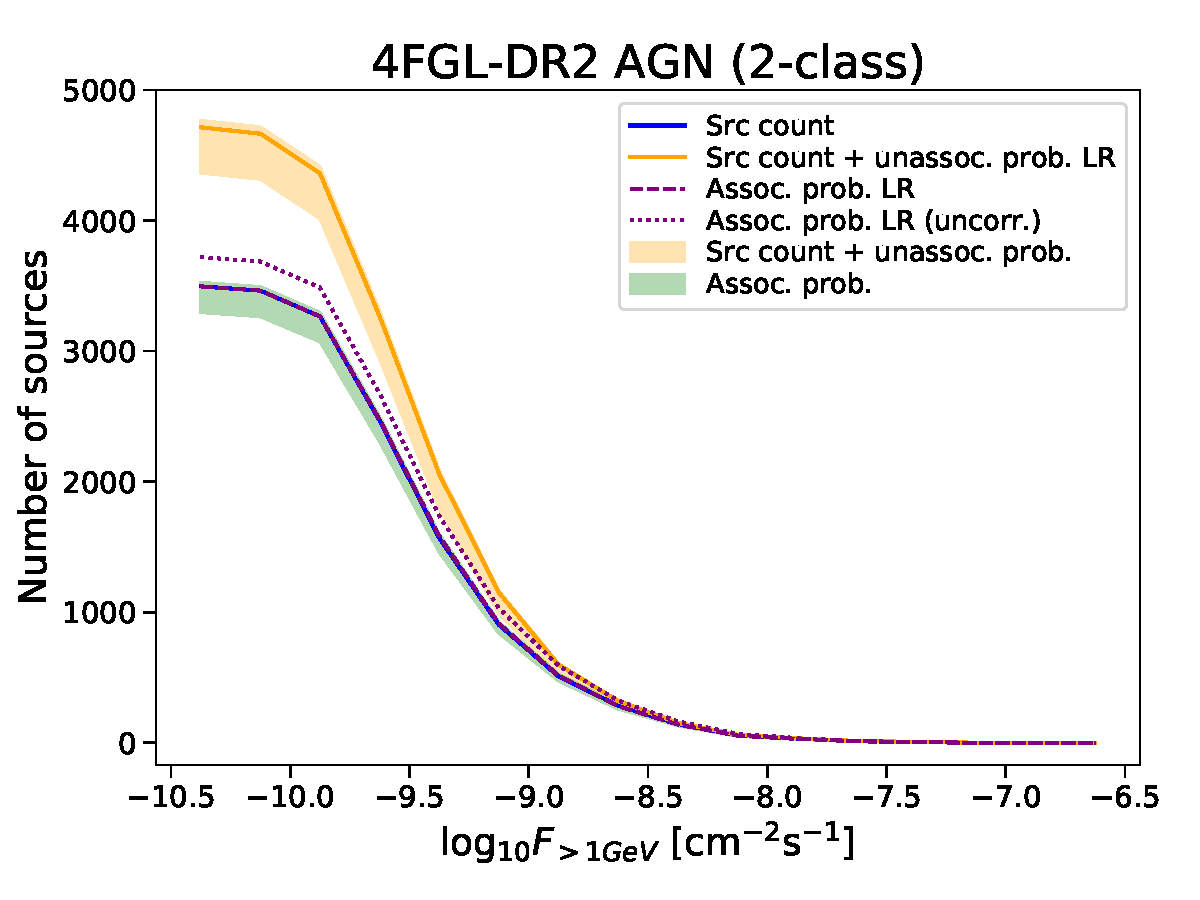
\includegraphics[width=0.45\textwidth]{plots/N_logS_4FGL-DR2_AGN_add_os.pdf}
\caption{Cumulative number of sources as a function of their flux. Green bands show the envelope of the sum of class probabilities for associated sources, while orange bands show the sum of counts of associated sources (blue solid line) plus the sum of probabilities for unassociated sources. The curves with ``SP16'' in the labels are derived from the data in \cite{2016ApJ...820....8S}. For details see Section \ref{sec:dNdS}.}  
\label{fig:logN_logS}
\end{figure*}


\begin{figure}[h]
\center
%\hspace*{-1cm}
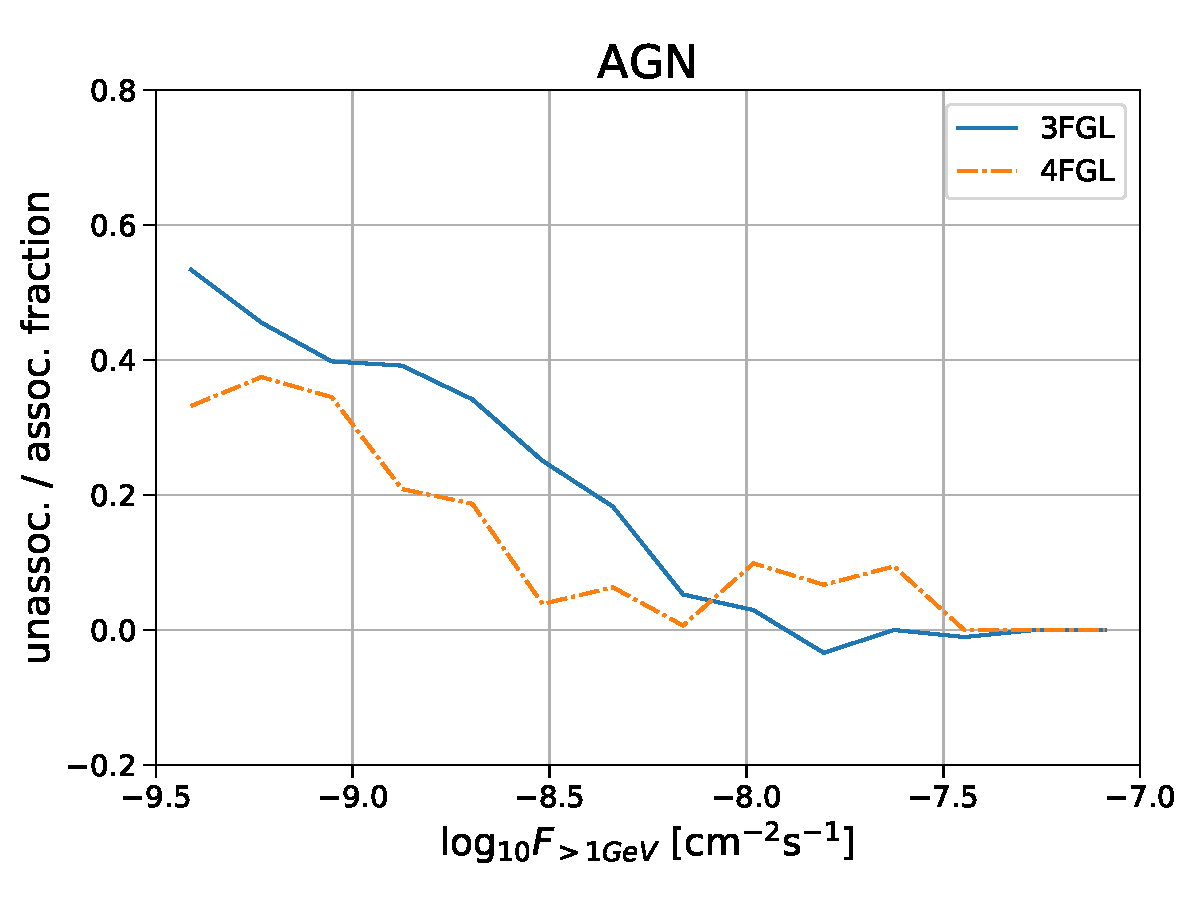
\includegraphics[width=0.45\textwidth]{plots/N_logS_diff_AGN.pdf}
%\hspace*{-1cm}
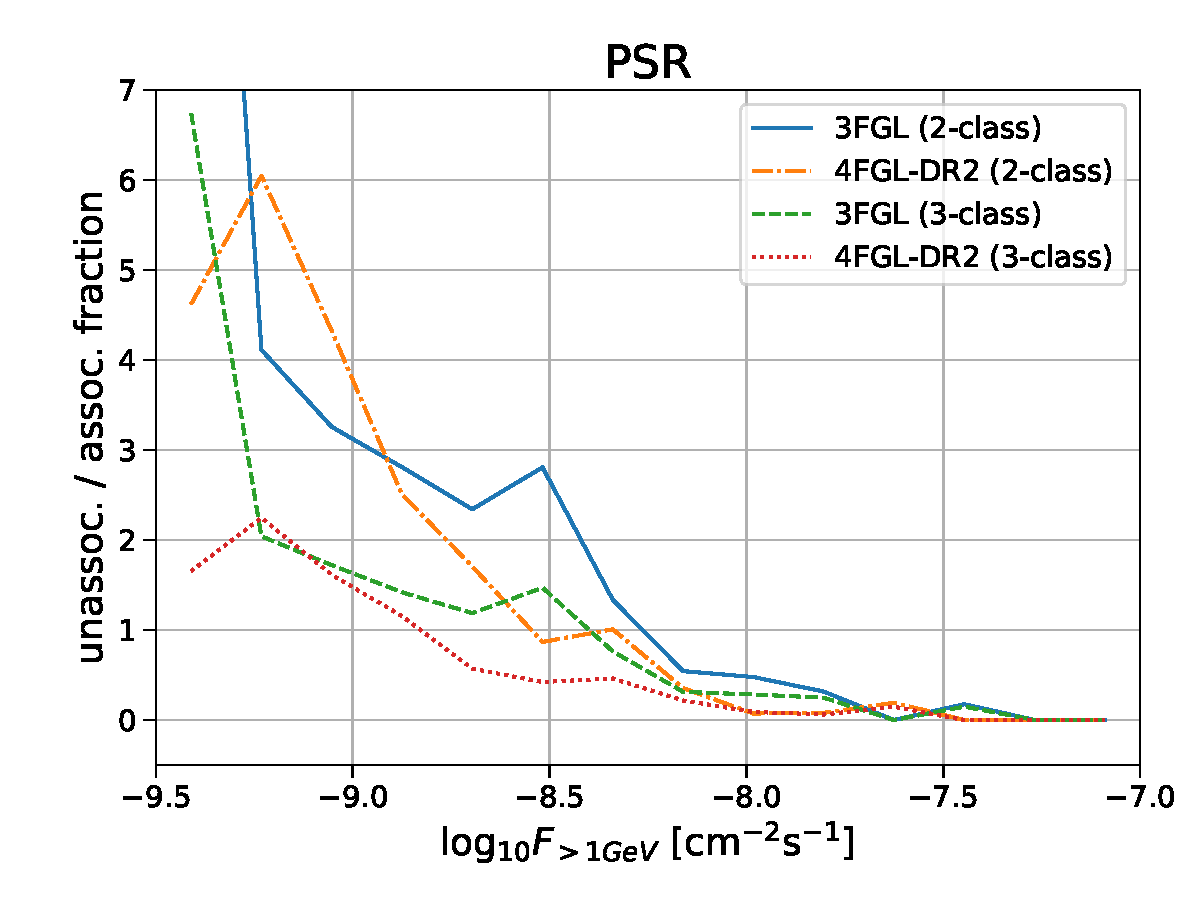
\includegraphics[width=0.45\textwidth]{plots/N_logS_diff_PSR.pdf}
\caption{Ratio of estimated number of AGNs and pulsars among unassociated sources corrected for the presence of other sources (Equation (\ref{eq:unassoc_ev})) to the counts of associated AGNs and pulsars respectively.}  
\label{fig:unass_vs_ass_frac}
\end{figure}




In Figure \ref{fig:logN_logS} we show the cumulative number of AGNs and pulsars with flux above 1 GeV larger than the
value on the x-axis.
Solid blue lines show the actual counts of sources (AGNs or pulsars) in the 3FGL and 4FGL catalogs.
As a consistency check of the method, we calculate the AGN- and PSR-like probabilities for associated sources.
The sum of probabilities (uncorrected for sources other than AGNs and pulsars) for LR algorithm are shown by dotted purple lines.
In order to correct the expected number of AGNs among associated sources for AGN-like probabilities in ``other'' sources, 
we subtract the corresponding AGN-like probabilities in each flux band:

\be
\lb{eq:assoc_ev}
N_{\rm AGN}^{\rm ass}  = \sum_{i \in \rm ass} p^i_{\rm AGN}\,\, - \sum_{i \in \rm ass\,other} p^i_{\rm AGN}.
\ee
The corrected sums of probabilities for LR method are shown by dashed purple lines.
The green bands show the envelope of the sums of corrected probabilities for the eight methods used in this paper.
We see that the counts of associated sources, AGNs and pulsars, are consistent with the expected number of associated sources
calculated from the class probabilities of associated sources.
This conclusion is not very surprising since we used associated sources for training of ML algorithms.
It is important to note that correction for ``other'' sources is important for consistency of the sum of probabilities and the number of associated sources.
We have also compared the sums of probabilities for the 3FGL associated sources in \cite{2016ApJ...820....8S}.
%\footnote{The data is downloaded from \url{https://www.physics.hku.hk/~pablo/pulsarness.html}.} !!! resolve the footnote issue?
The sum of probabilities for associated sources in the LR case uncorrected for ``other'' sources are shown by dotted black line,
while the sums corrected for ``other'' sources are shown by black dash-dotted lines.
The gray band is the envelope of the two methods (LR and RF) used by \cite{2016ApJ...820....8S}.
We see that the sum of probabilities for pulsars overpredicts the pulsar counts in 3FGL, 
while correction for ``other'' sources makes the prediction consistent with the counts of pulsars.

The predictions for the number of AGNs and pulsars among the unassociated sources corrected for ``other'' sources 
added to the 3FGL and 4FGL source counts are shown by solid orange lines (for the LR case).
The orange bands show the corresponding envelopes for the eight ML methods.
We assume that the fractional contribution of other sources is the same for associated and unassociated sources in the different flux bands.
Thus, the correction for the presence of other sources is calculated similarly to the associated sources in Equation \ref{eq:assoc_ev},
but we adjust for the fact that there are fewer unassociated than associated sources, i.e., 
the correction is assumed to be proportionally smaller.
In particular, the number of AGNs among unassociated sources in a flux band $\Delta F$ is estimated as

\be
\lb{eq:unassoc_ev}
N_{\rm AGN}^{\rm unass} = \sum_{i \in \rm unass} p^i_{\rm AGN}\,\, - \sum_{i \in \rm ass\,other} p^i_{\rm AGN} \cdot 
\frac{N_{\rm unass}}{N_{\rm ass}}
\ee
where all probabilities and the numbers of sources are computed for sources with flux inside $\Delta F$.
The first term is the sum of AGN-like probabilities among the unassociated sources,
while the second term is the sum of AGN-like probabilities among associated ``other'' sources rescaled by the total number
of unassociated and associated sources in this flux band.
The expected number of pulsars among the unassociated sources is calculated analogously.
The corresponding sums of associated source counts plus the expected number of sources calculated with LR method of \cite{2016ApJ...820....8S} 
and corrected for other sources are shown by dashed grey lines.


We predict that the expected number of pulsars among the unassociated sources in the 3FGL catalog
is $267 \pm 110$, where the range is the envelop of the sums of probabilities in Equation (\ref{eq:unassoc_ev})
for different ML methods (including oversampling) corrected for other sources among the unassociated sources.
The expected number of pulsars among the unassociated sources in the 4FGL catalog corrected for other sources is 
$386 \pm 179$.
These numbers are larger than the number of associated PSRs without missing values (164 in 3FGL and 237 in 4FGL).
Even at the lower range of expected numbers of pulsars among unassociated sources, there are potentially as many pulsars
as there are associated ones.

We note that according to Table \ref{tab:3FGL_prediction}, the number of unassociated 3FGL sources 
with $p_{\rm PSR} > 0.5$ for all four ML algorithms is 96 (83), while there are 332 (309.5) sources with mixed classification,
uncorrected (corrected) for other sources.
The number of sources with mixed classification (309.5 for 3FGL or 475.5 for 4FGL)
is larger than the range of values for the expected number of pulsars calculated for the sum of probabilities 
(220 for 3FGL or 358 for 4FGL).
It means that the decision which sources are considered to be more likely pulsars is more sensitive to the choice of the ML method
and the probability threshold than the expected number of pulsars calculated from the sum of probabilities.

We also note that the probabilistic classification mostly affects sources with smaller fluxes,
which we illustrate in Figure \ref{fig:unass_vs_ass_frac}, where we show that the ratio of expected number of AGNs and pulsars among 
unassociated sources computed according to Eq. \ref{eq:unassoc_ev} using LR method without oversampling to the number of associated 
sources decreases as the flux increases.
Negative values (e.g., at high fluxes for AGNs) are due to subtraction of probabilities for the ``other'' associated sources.

\begin{figure*}[h]
\center
%\hspace*{-1cm}
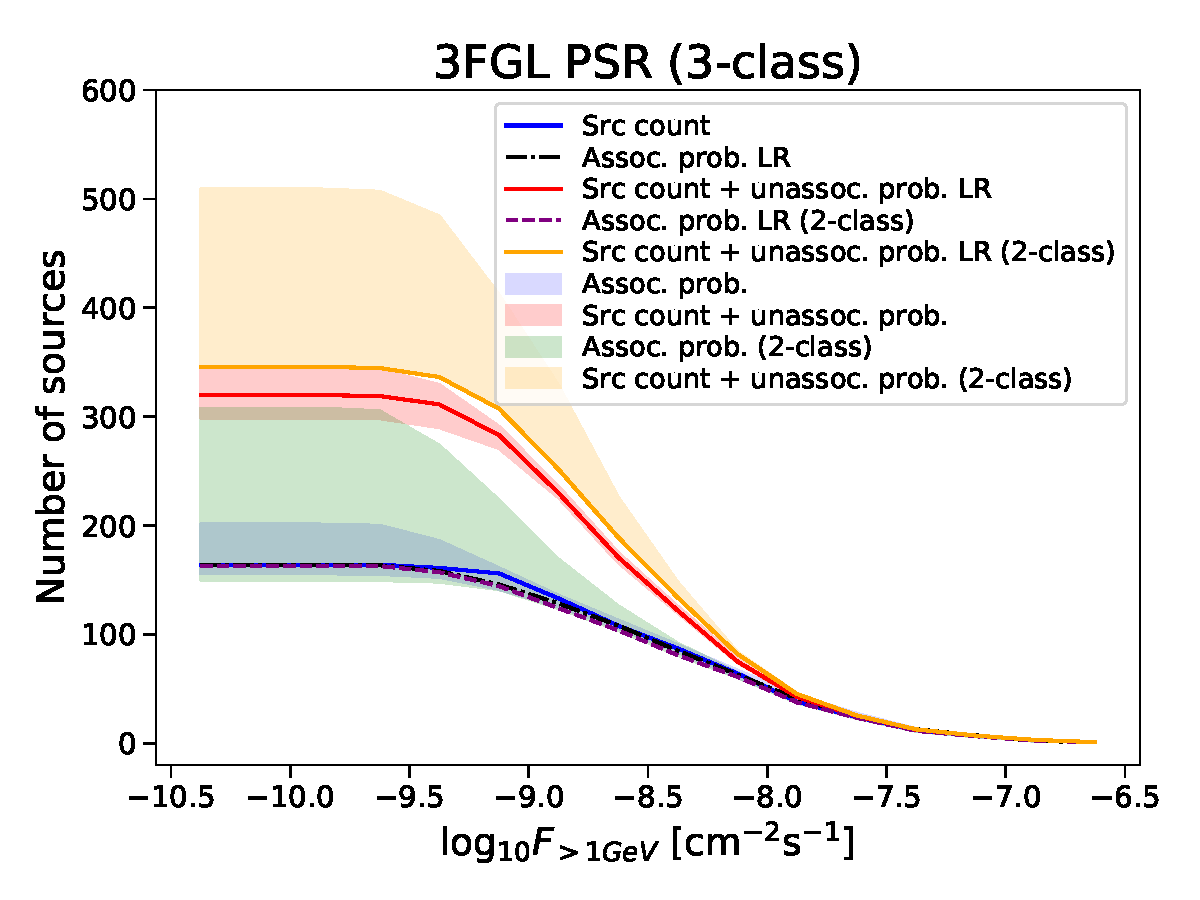
\includegraphics[width=0.45\textwidth]{plots/N_logS_3FGL_PSR_3classes.pdf}
%\hspace*{-1cm}
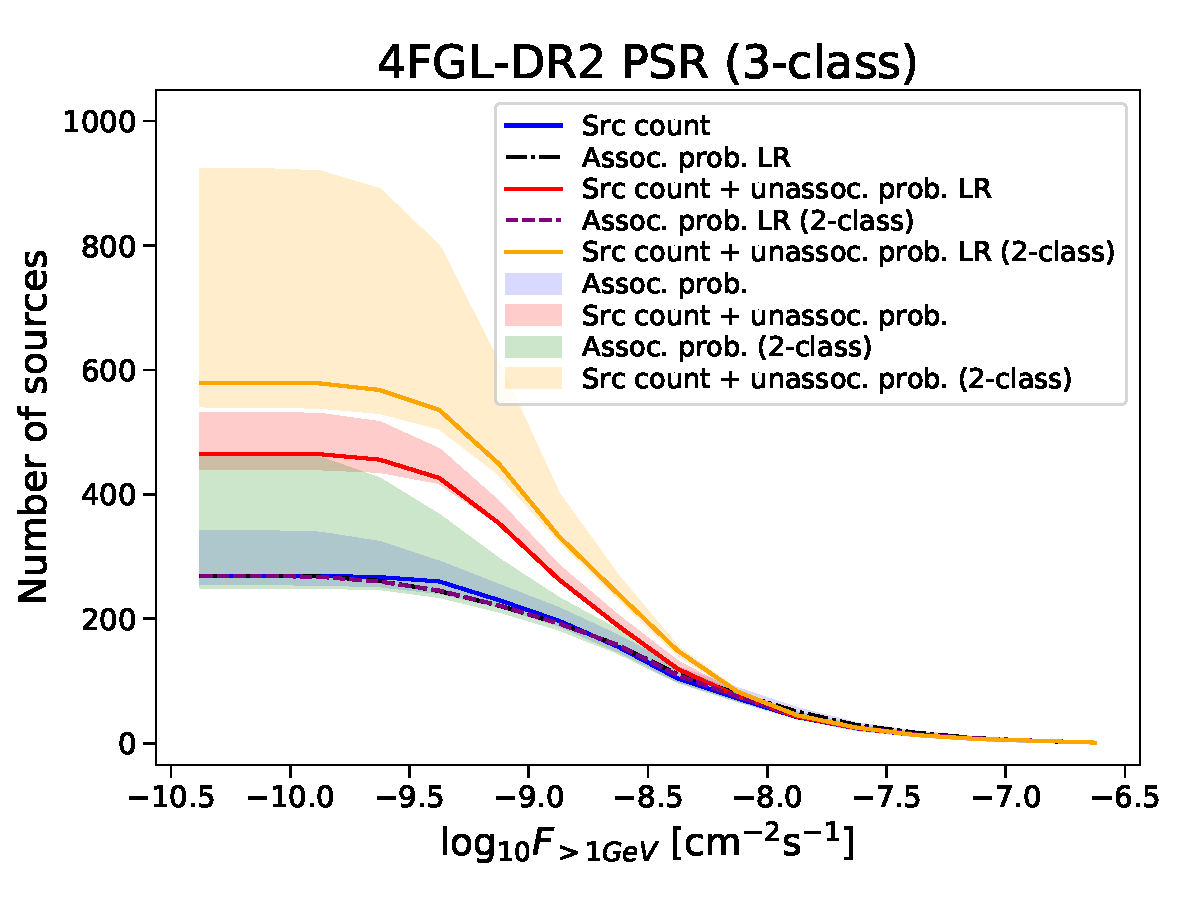
\includegraphics[width=0.45\textwidth]{plots/N_logS_4FGL-DR2_PSR_3classes.pdf} \\
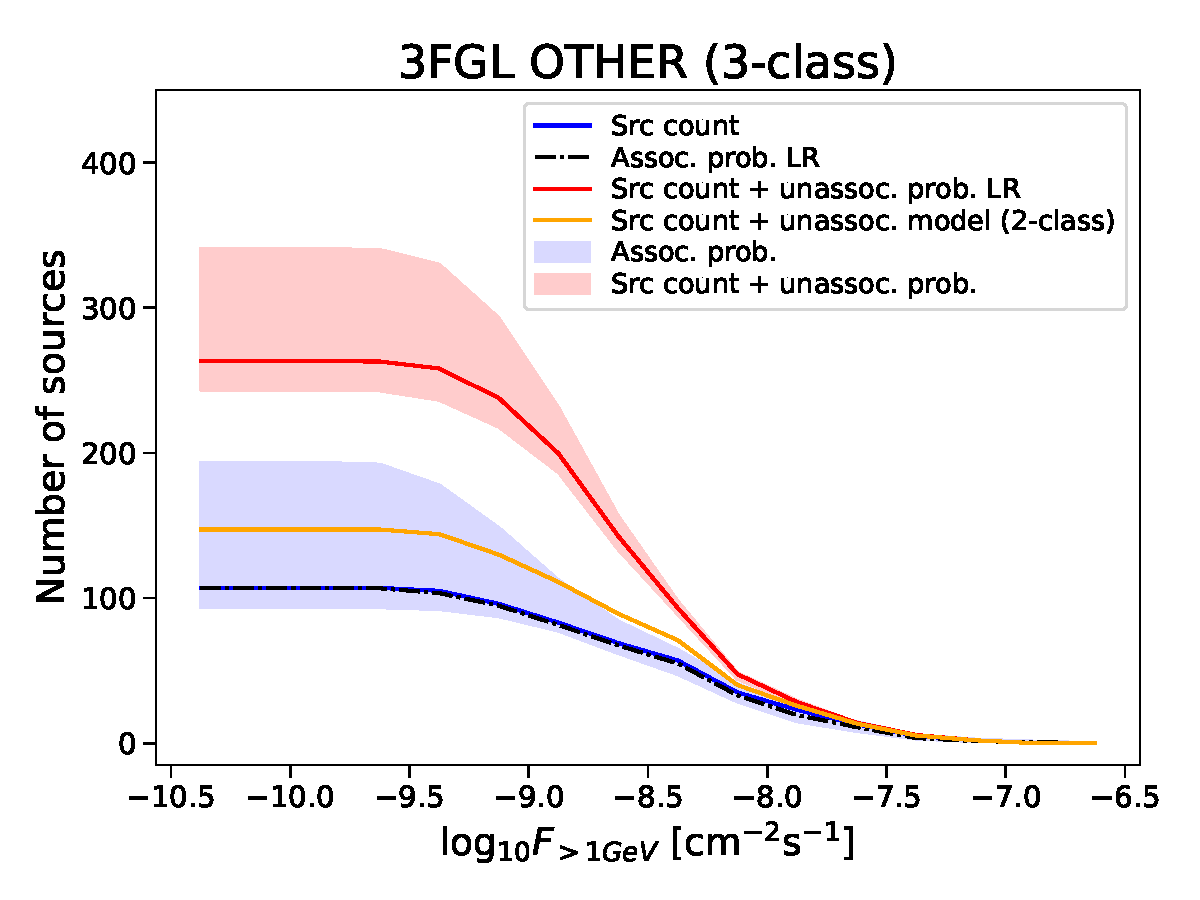
\includegraphics[width=0.45\textwidth]{plots/N_logS_3FGL_OTHER_3classes.pdf}
%\hspace*{-1cm}
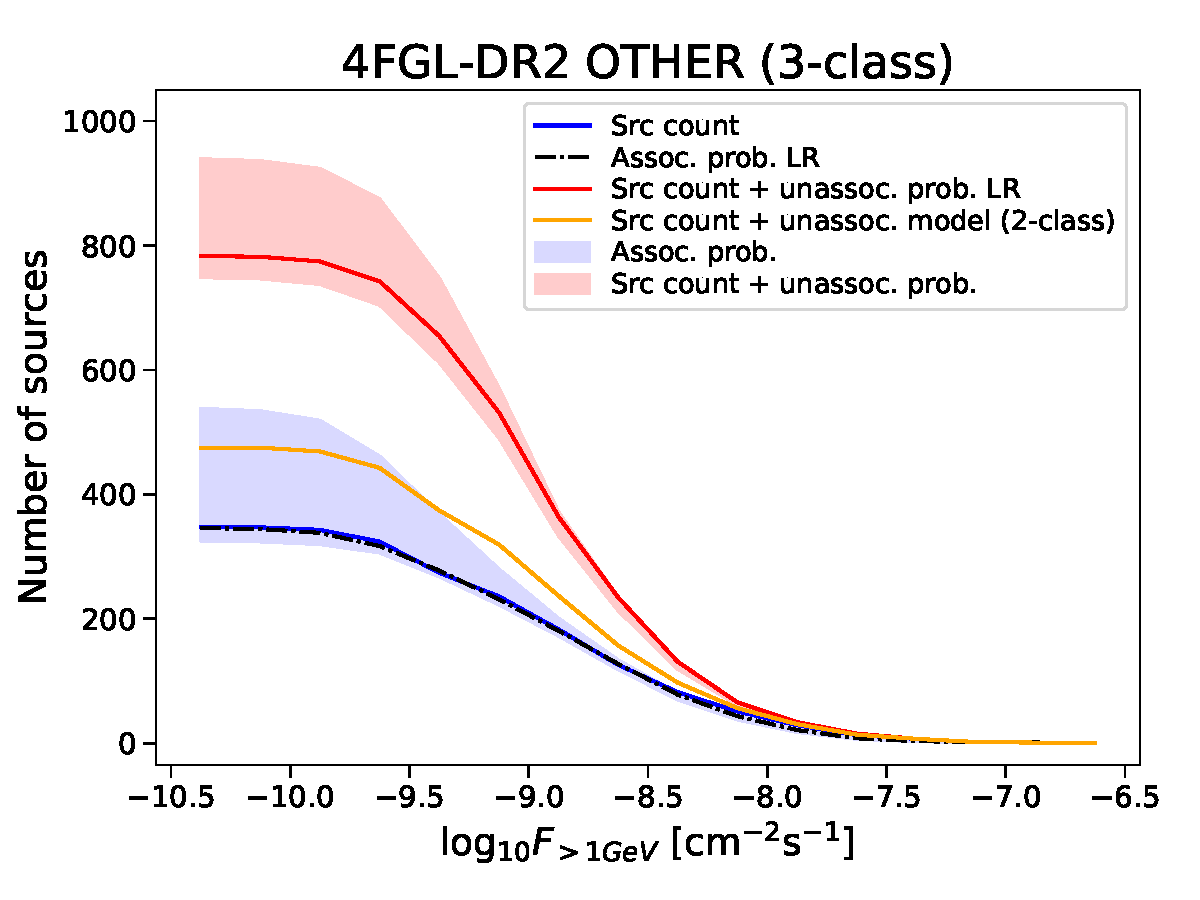
\includegraphics[width=0.45\textwidth]{plots/N_logS_4FGL-DR2_OTHER_3classes.pdf}
\caption{Cumulative number of sources as a function of their flux. Green bands show the envelope of the sum of class probabilities for associated sources, while orange bands show the sum of counts of associated sources (blue solid line) plus the sum of probabilities for unassociated sources. The curves with ``SP16'' in the labels are derived from the data in \cite{2016ApJ...820....8S}. For details see Section \ref{sec:dNdS}.}  
\label{fig:logN_logS_3classes}
\end{figure*}


\subsection{Latitude and longitude profiles}
\lb{sec:lat-lon-profiles}

\begin{figure*}[h]
\center
%\hspace*{-1cm}
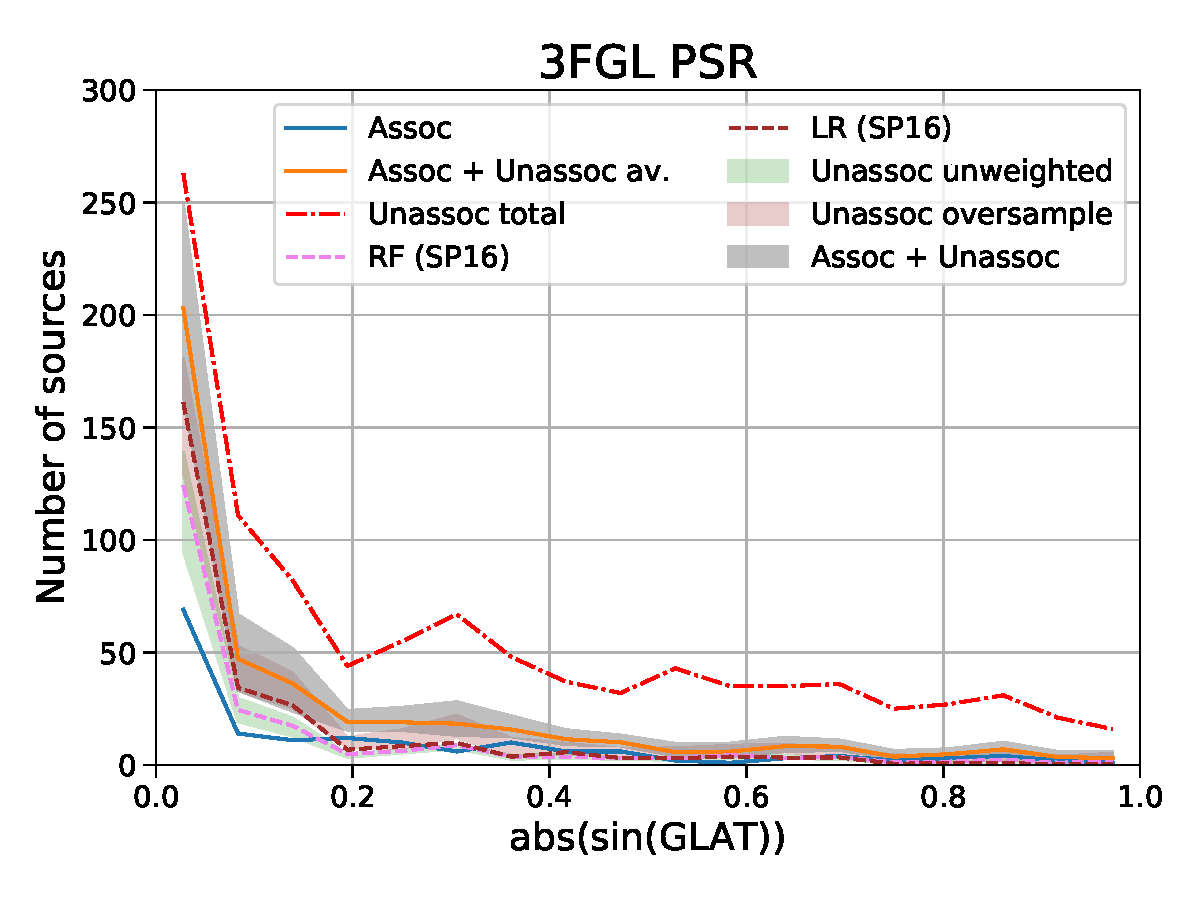
\includegraphics[width=0.45\textwidth]{plots/lat_profile_PSR_3FGL_oversample.pdf}
%\hspace*{-1cm}
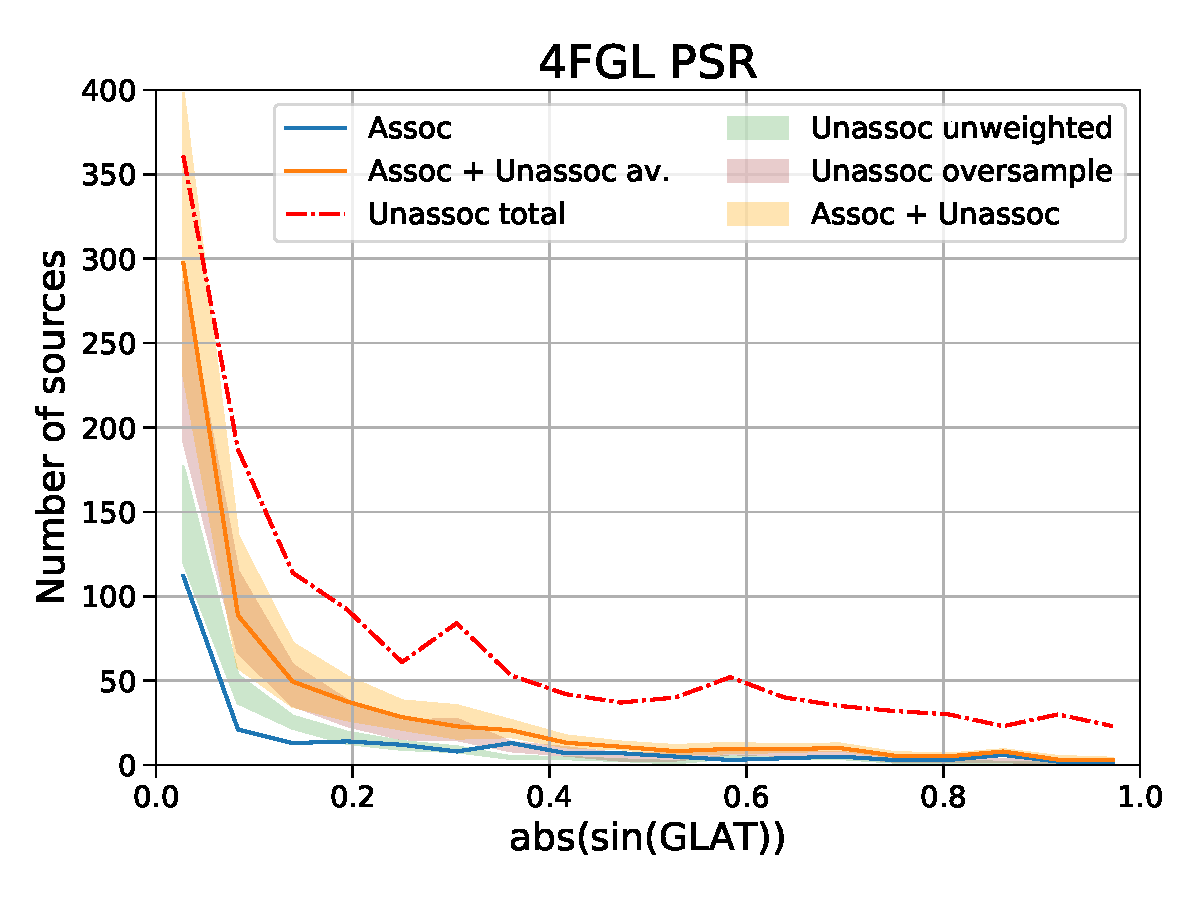
\includegraphics[width=0.45\textwidth]{plots/lat_profile_PSR_4FGL_oversample.pdf} \\
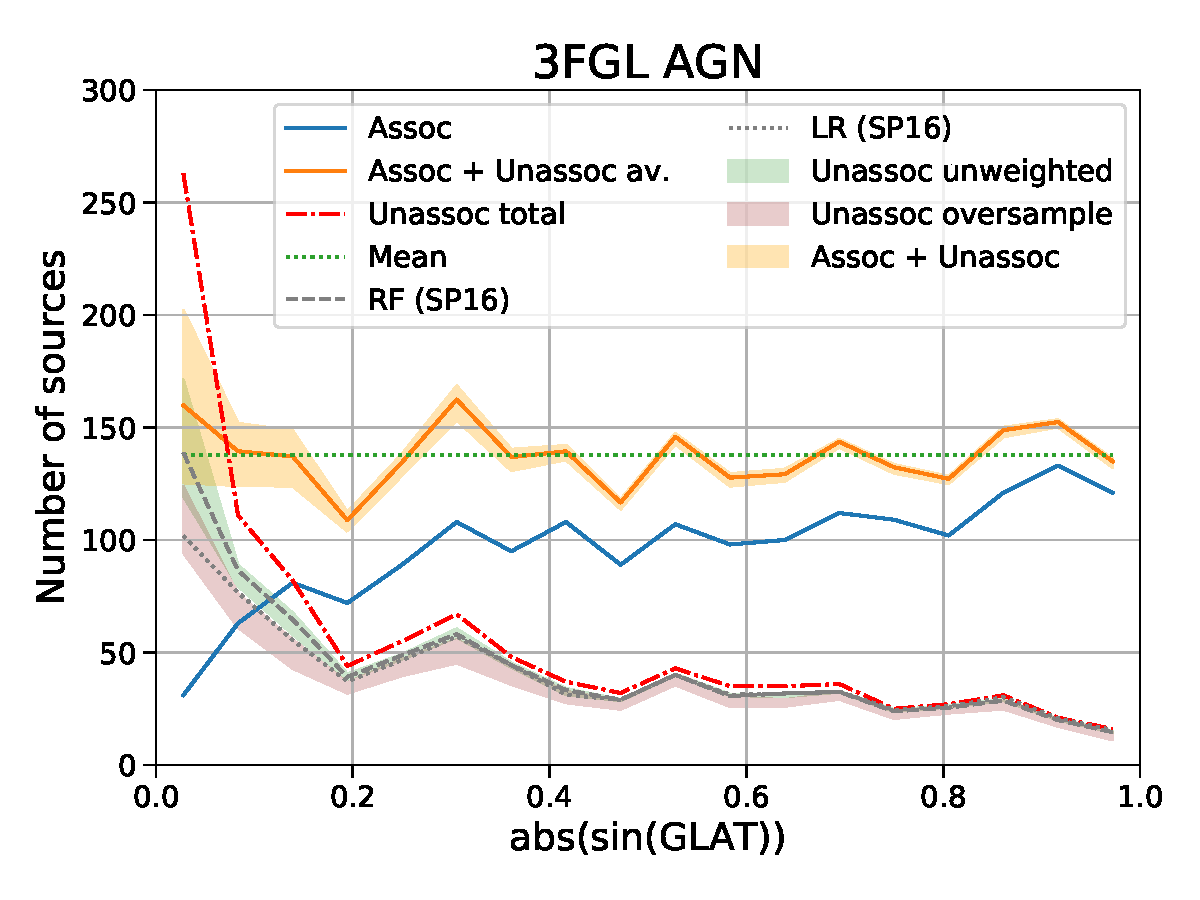
\includegraphics[width=0.45\textwidth]{plots/lat_profile_AGN_3FGL_oversample.pdf}
%\hspace*{-1cm}
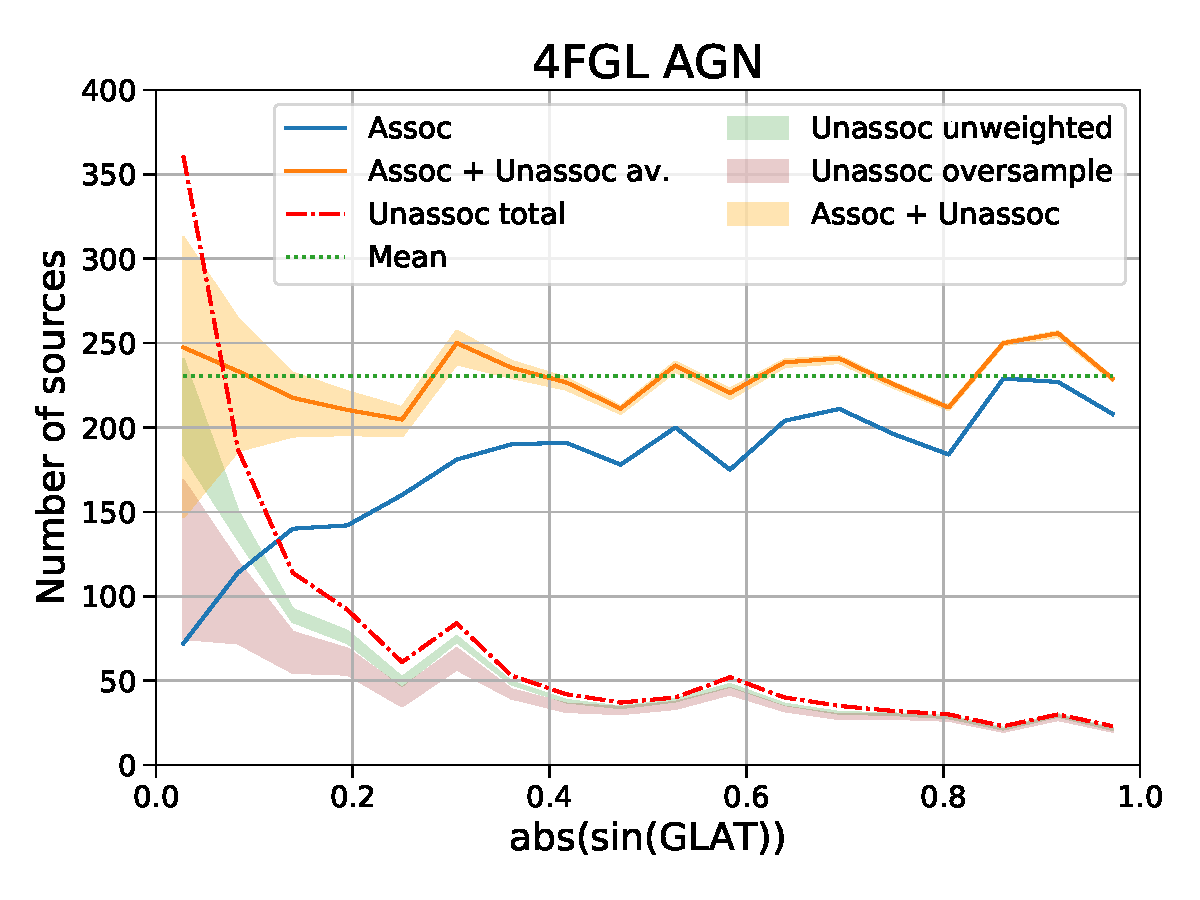
\includegraphics[width=0.45\textwidth]{plots/lat_profile_AGN_4FGL_oversample.pdf}
\caption{Latitude profiles of source counts. Blue solid line -- associated 3FGL and 4FGL sources. Red dash-dotted line -- all unassociated sources. Green (red) band -- envelope of sums of class probabilities for unassociated sources for the four ML algorithms without (with) oversampling. Orange solid line (band) -- average (envelope) of sums of class probabilities for the eight ML methods with and without oversampling added to the source count of associated sources. 
Green dashed line on the AGN plots -- mean of the sum of counts of associated sources and the average of the expectations for counts of unassociated sources (mean of the orange solid line).
Gray dashed (dotted) line -- RF (LR) sums of class probabilities from \cite{2016ApJ...820....8S}.
For details see Section \ref{sec:lat-lon-profiles}. }  
\label{fig:lat_profile}
\end{figure*}



\begin{figure*}[h]
\center
%\hspace*{-1cm}
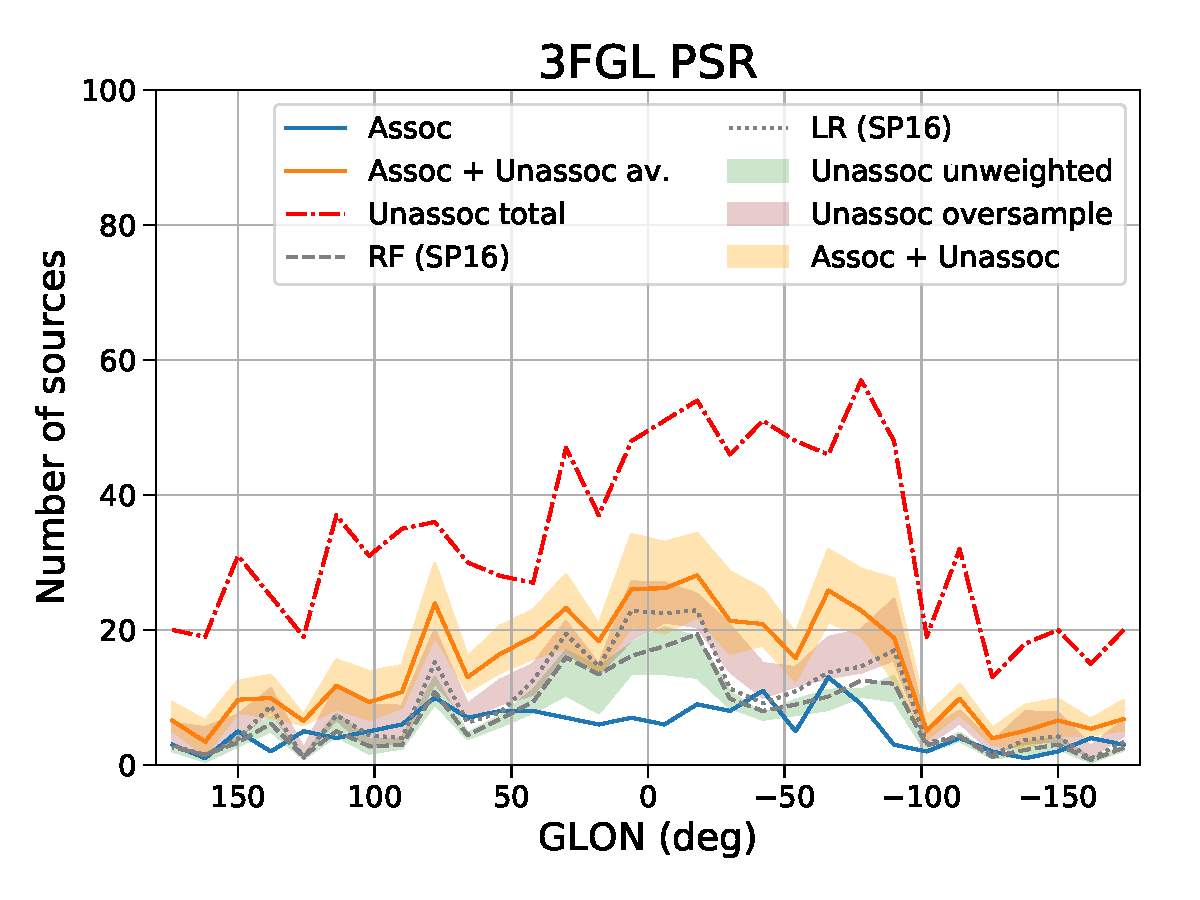
\includegraphics[width=0.45\textwidth]{plots/lon_profile_PSR_3FGL_oversample.pdf}
%\hspace*{-1cm}
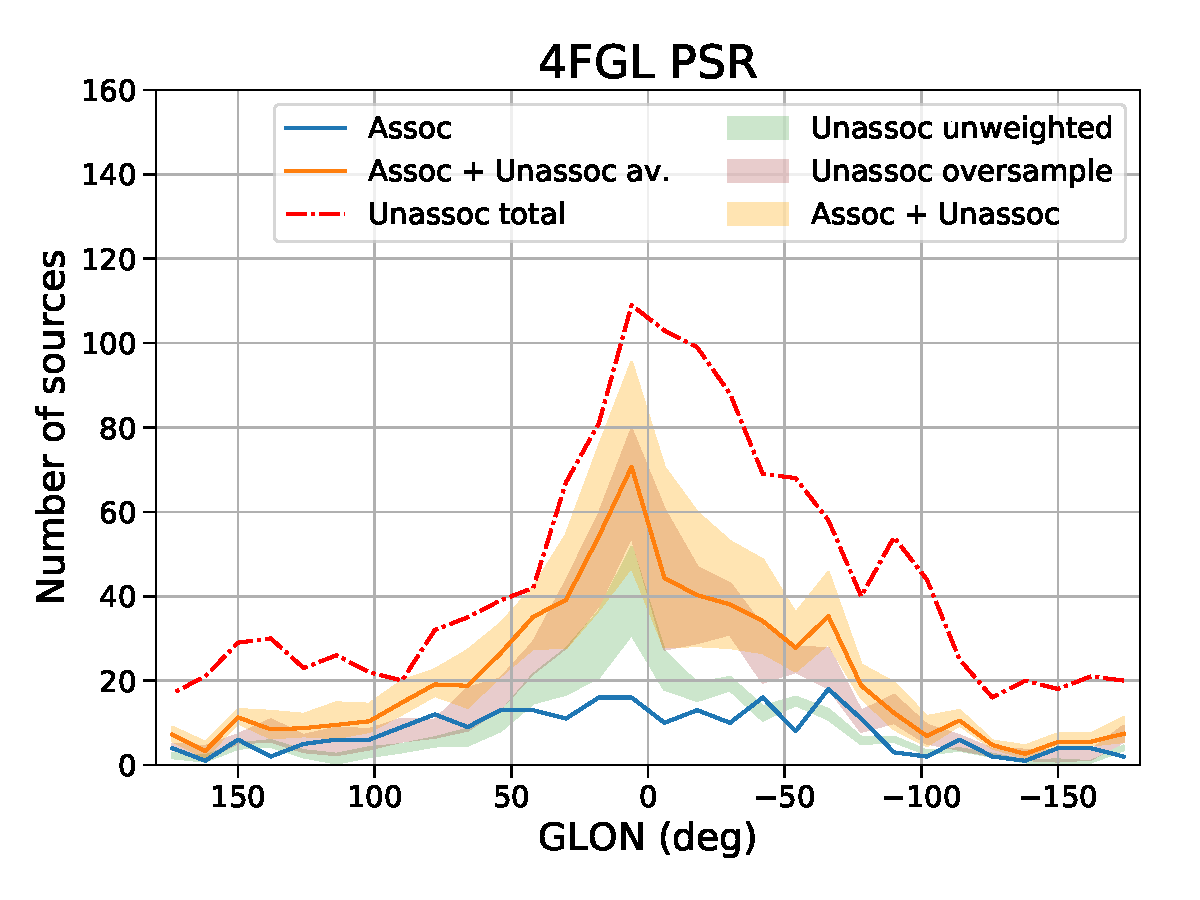
\includegraphics[width=0.45\textwidth]{plots/lon_profile_PSR_4FGL_oversample.pdf} \\
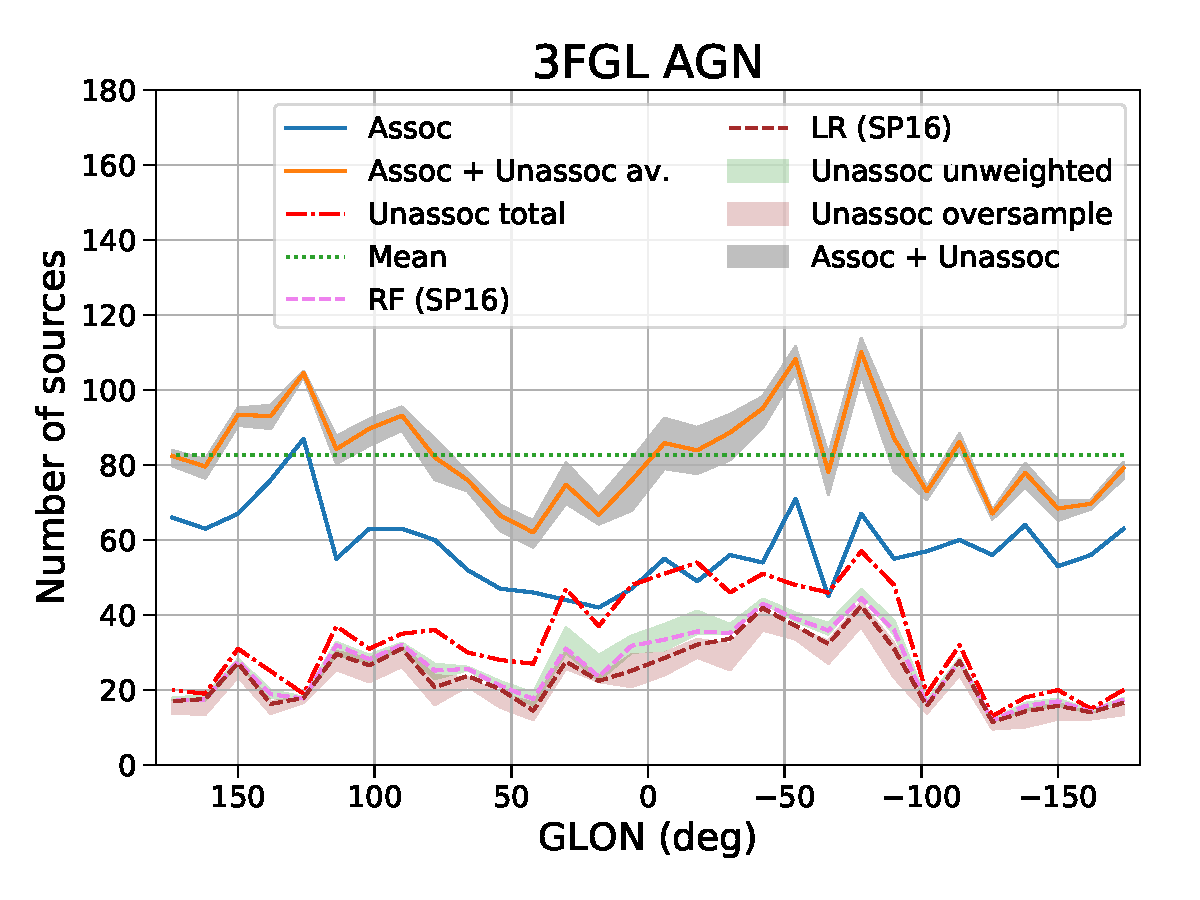
\includegraphics[width=0.45\textwidth]{plots/lon_profile_AGN_3FGL_oversample.pdf}
%\hspace*{-1cm}
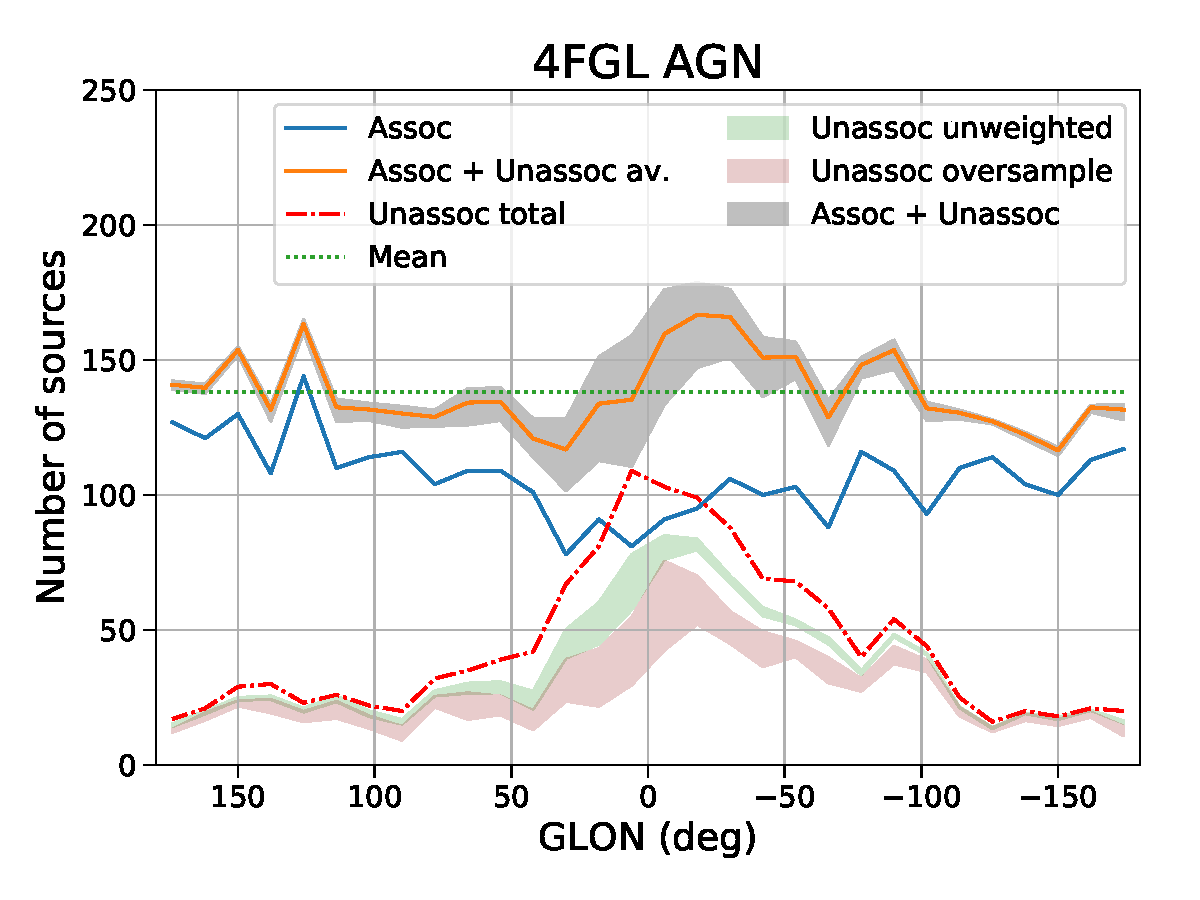
\includegraphics[width=0.45\textwidth]{plots/lon_profile_AGN_4FGL_oversample.pdf}
\caption{Longitude profiles of source counts. For the definition of labels see Figure \ref{fig:lat_profile}.}  
\label{fig:lon_profile}
\end{figure*}


In this section we show Galactic latitude and longitude profiles of the distributions of associated and unassociated sources.
In Figure \ref{fig:lat_profile} we present the source counts as a function of ${\rm abs(sin(GLAT))}$,
where we use 20 bins, i.e., each bin corresponds to a solid angle of $4 \pi / 20$. 
Solid blue lines show counts of associated sources in 3FGL and 4FGL catalogs.
It is interesting to note that the density of associated AGNs is decreasing near the Galactic plane.
The total counts of unassociated sources are shown by red dash-dotted lines.
Green shaded areas show the envelopes of sums of probabilities for AGN- and PSR-like sources for the four 
algorithms without oversampling, while the red shaded areas show the envelope for the four algorithms 
with oversampling.
The classifications of 3FGL sources by \cite{2016ApJ...820....8S} are shown by gray dashed (RF) and dotted (LR) lines.
In this section we do not perform a correction for the presence of other sources among the unassociated ones.
The numbers of unassociated sources classified as AGNs and PSRs grow towards the Galactic plane (GP).
Within $\approx 4^\circ\!\!.5$ from the GP the expected number of PSRs is about the same as the number of AGNs among unassociated sources (the first data point on the left).
At high latitudes, most of unassociated sources are classified as AGNs.
It is interesting to note, that according to Table \ref{tab:feat_imp}, GLAT is one of the least important features for the RF algorithm.
It can be a posteriori explained by the fact that
 the density of AGNs is such that even in the GP the expected number of AGNs is comparable to the expected number of PSRs.

Orange shaded areas show the sum of the source counts and the expected number of sources for the eight methods (both with and without oversampling).
The average among the eight methods added to the counts of associated sources is shown by solid orange line 
(for AGNs we also show the mean of these points by dotted green line).
We find that the number of associated AGNs is decreasing towards the GP, the expected number of AGNs among unassociated sources is increasing towards the GP, but the sum of the two is relatively uniform as a function of Galactic latitude.


In Figure \ref{fig:lon_profile} we show plots analogous to Figure \ref{fig:lat_profile} for Galactic longitudes.
We note that there is a significant increase in the number of unassociated sources in the 4FGL catalog for $|\ell | \lesssim 50^\circ$.
It leads to a large expected number of pulsars among unassociated sources for these longitudes.
The number of associated AGNs is smaller than average for $|\ell | \lesssim 50^\circ$, while the expected number of AGNs among unassociated sources is larger than average for these longitudes.
The sum of the two is relatively uniform, with a possible overprediction of AGNs in the unassociated sources in the 4FGL catalog for \mbox{$-50^\circ < \ell < 0^\circ$}.











\section{Conclusions}
\lb{sec:conclusions}

In this paper we determine the probabilities of classification of unassociated sources in the 3FGL and 4FGL-DR2 \Fermi-LAT catalogs
into two (AGNs and pulsars) and three (AGNs, pulsars, and other sources) classes.
The probabilities are calculated with 8 different ML methods: RF, BDT, LR and NN -- each algorithm with and without oversampling during training.
The algorithms were trained and tested with associated sources.
We have scanned some meta-parameters of the algorithms, such as depth of the trees, the number of trees, the number of neurons, in order to determine optimal parameters which do not create overfitting of data and provide good accuracy of classification.
The accuracies, which we obtained for the 3FGL catalog for the four algorithms without oversampling in the 2-class case are about 97\%, and between 93\% and 97\% with oversampling.
We have also checked the accuracy of classification by selecting unassociated sources in 3FGL, which have associations in 4FGL-DR2.
If we take the 4FGL-DR2 associations as the true classes, then the accuracies of classification in this subset of sources 
without (with) oversampling are between 90\% and 91\% (85\% and 92\%).
Most of misclassified sources in this comparison have spectral parameters in 3FGL which are typical of the other class (Figure \ref{fig:3FGL_vs_4FGL_classes}), i.e.,  the misclassification can be due to problems with reconstructing the spectrum of the sources.
In the 3-class classification, the testing accuracies for the 3FGL catalog are between 92\% and 94\% (both with and without oversampling), while comparison with 4FGL-DR2 give accuracy between 82\% and 85\%. For the 4FGL-DR2 classifications, the testing accuracy is between 90\% and 93\% (both with and without oversampling). If one takes into account that all other sources are misclassified in the 2-class case, then the 3-class case provides an improvement in accuracy of 1\% to 5\%.

We have created four catalogs with probabilistic classifications of sources: based on 3FGL and on 4FGL-DR2 with 2- and 3-class classifications.
For each source and for each class we report class probabilities for each of the eight ML methods (with and without oversampling). 
We also provide individual standard deviations for all classification probabilities by using sample average over selection of training and testing datasets.
We report the classification probabilities not only for the unassociated sources, but also for the associated ones, which can be used to find outliers.
An advantage of such probabilistic classification is that a threshold on probability for selecting, e.g., pulsar candidates, can be chosen by the user based on his or her needs.
For example, in a search of new pulsars, one can select a low threshold in order to avoid missing possible pulsars.
In a derivation of an average property of the class, e.g., spectral index or cutoff energy, one can select a high threshold in order to avoid contamination from the other classes.


As an example of the application of the probabilistic catalogs, we derive the expected number of sources in the catalog as a function of their flux, including the unassociated sources.
As a consistency check, we compare the counts of associated sources to the sums of probabilities for the associated ones.
We find that correcting for the contribution of other sources in the 2-class case plays an important role for the estimation of the expected number of sources in a particular class.
We find the total expected number of AGNs and pulsars in the 3FGL and 4FGL catalogs by adding the class probabilities for the unassociated sources in the 2- and 3-class cases to the source counts of associated sources and correcting in the 2-class case for the contribution of other classes in the unassociated sources.
In particular, we find that the total expected number of pulsars is about two times larger than the number of associated pulsars.

We plot the counts of associated sources and the expected numbers of AGNs, pulsars, and other sources among unassociated sources
as functions of Galactic latitude and longitude.
We find that the number of associated AGNs is decreasing towards low latitudes, while the expected number of AGNs among unassociated sources is increasing, so that the sum of the two is relatively uniform, as expected for extragalactic sources.


\subsection*{Acknowledgements}

The authors would like to thank Pablo Saz Parkinson and Jean Ballet for valuable discussions.
This work was in part supported by BMBF under the ErUM-Data project ``Innovative Digital Technologies for Research on Universe and Matter'' (grant number 05H18WERC1) and by DFG grant MA 8279/2-1.
We would like to acknowledge the use of the following software:
Astropy \citep[\url{http://www.astropy.org},][]{2013A&A...558A..33A}, 
matplotlib \citep{Hunter:2007}, 
scikit-learn [\url{https://scikit-learn.org/stable/about.html}], 
TOPCAT \citep{2005ASPC..347...29T}.


%\newpage
\bibliography{ML_3FGL_papers}  

\begin{appendix}
\section{Tests of additional meta-parameters}
\lb{sec:app}

In this appendix we discuss tests of some hyper-parameters, which had a relatively little effect on the 
accuracy of the algorithms. For these tests we use the 3FGL catalog.

LR algorithm has two hyper-parameters regularization and tolerance. 
%These features are the limit up to which one wants to go before accepting a solution. 
As can be seen in figure \ref{fig:LR_tol_reg} the effect on accuracy is less than 1\%. Therefore we used the default values for these parameters (tolerance is 1$e^{-4}$ and regularization parameter is set at 1).% \dima{If we mention the default value, we should say what the default values are}. 
\begin{figure}[h]
%\centerin
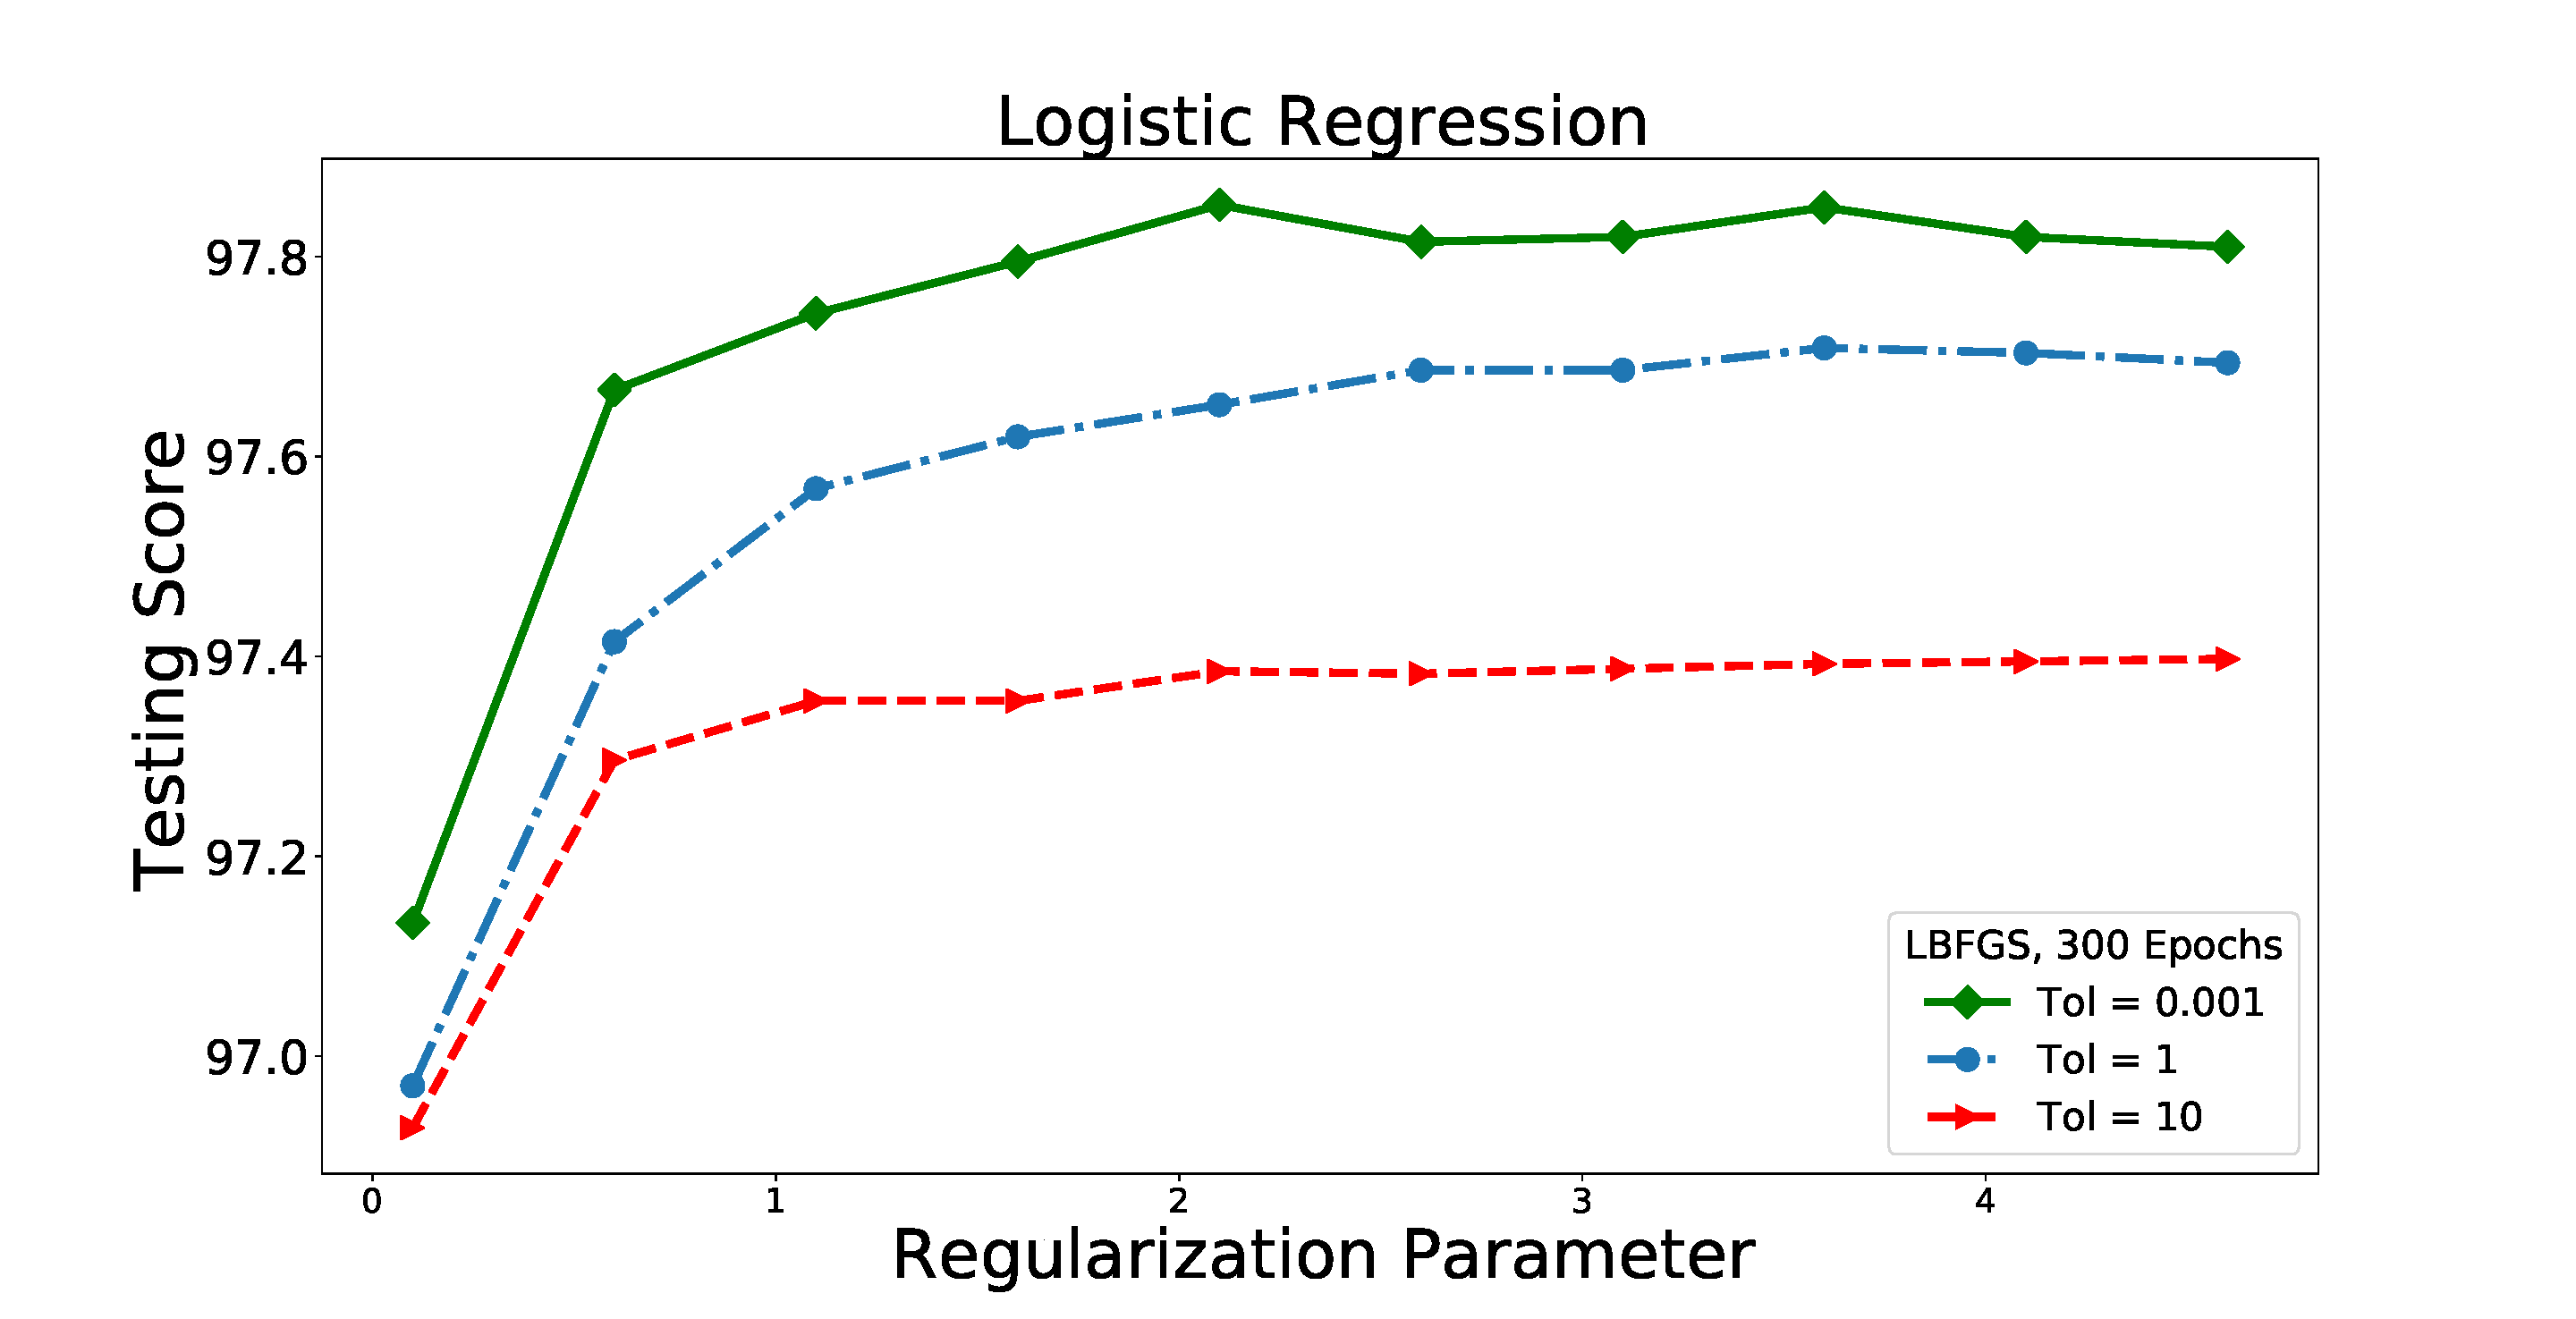
\includegraphics[width=\twopicsp\textwidth]{plots/lr_train_reg.pdf}
%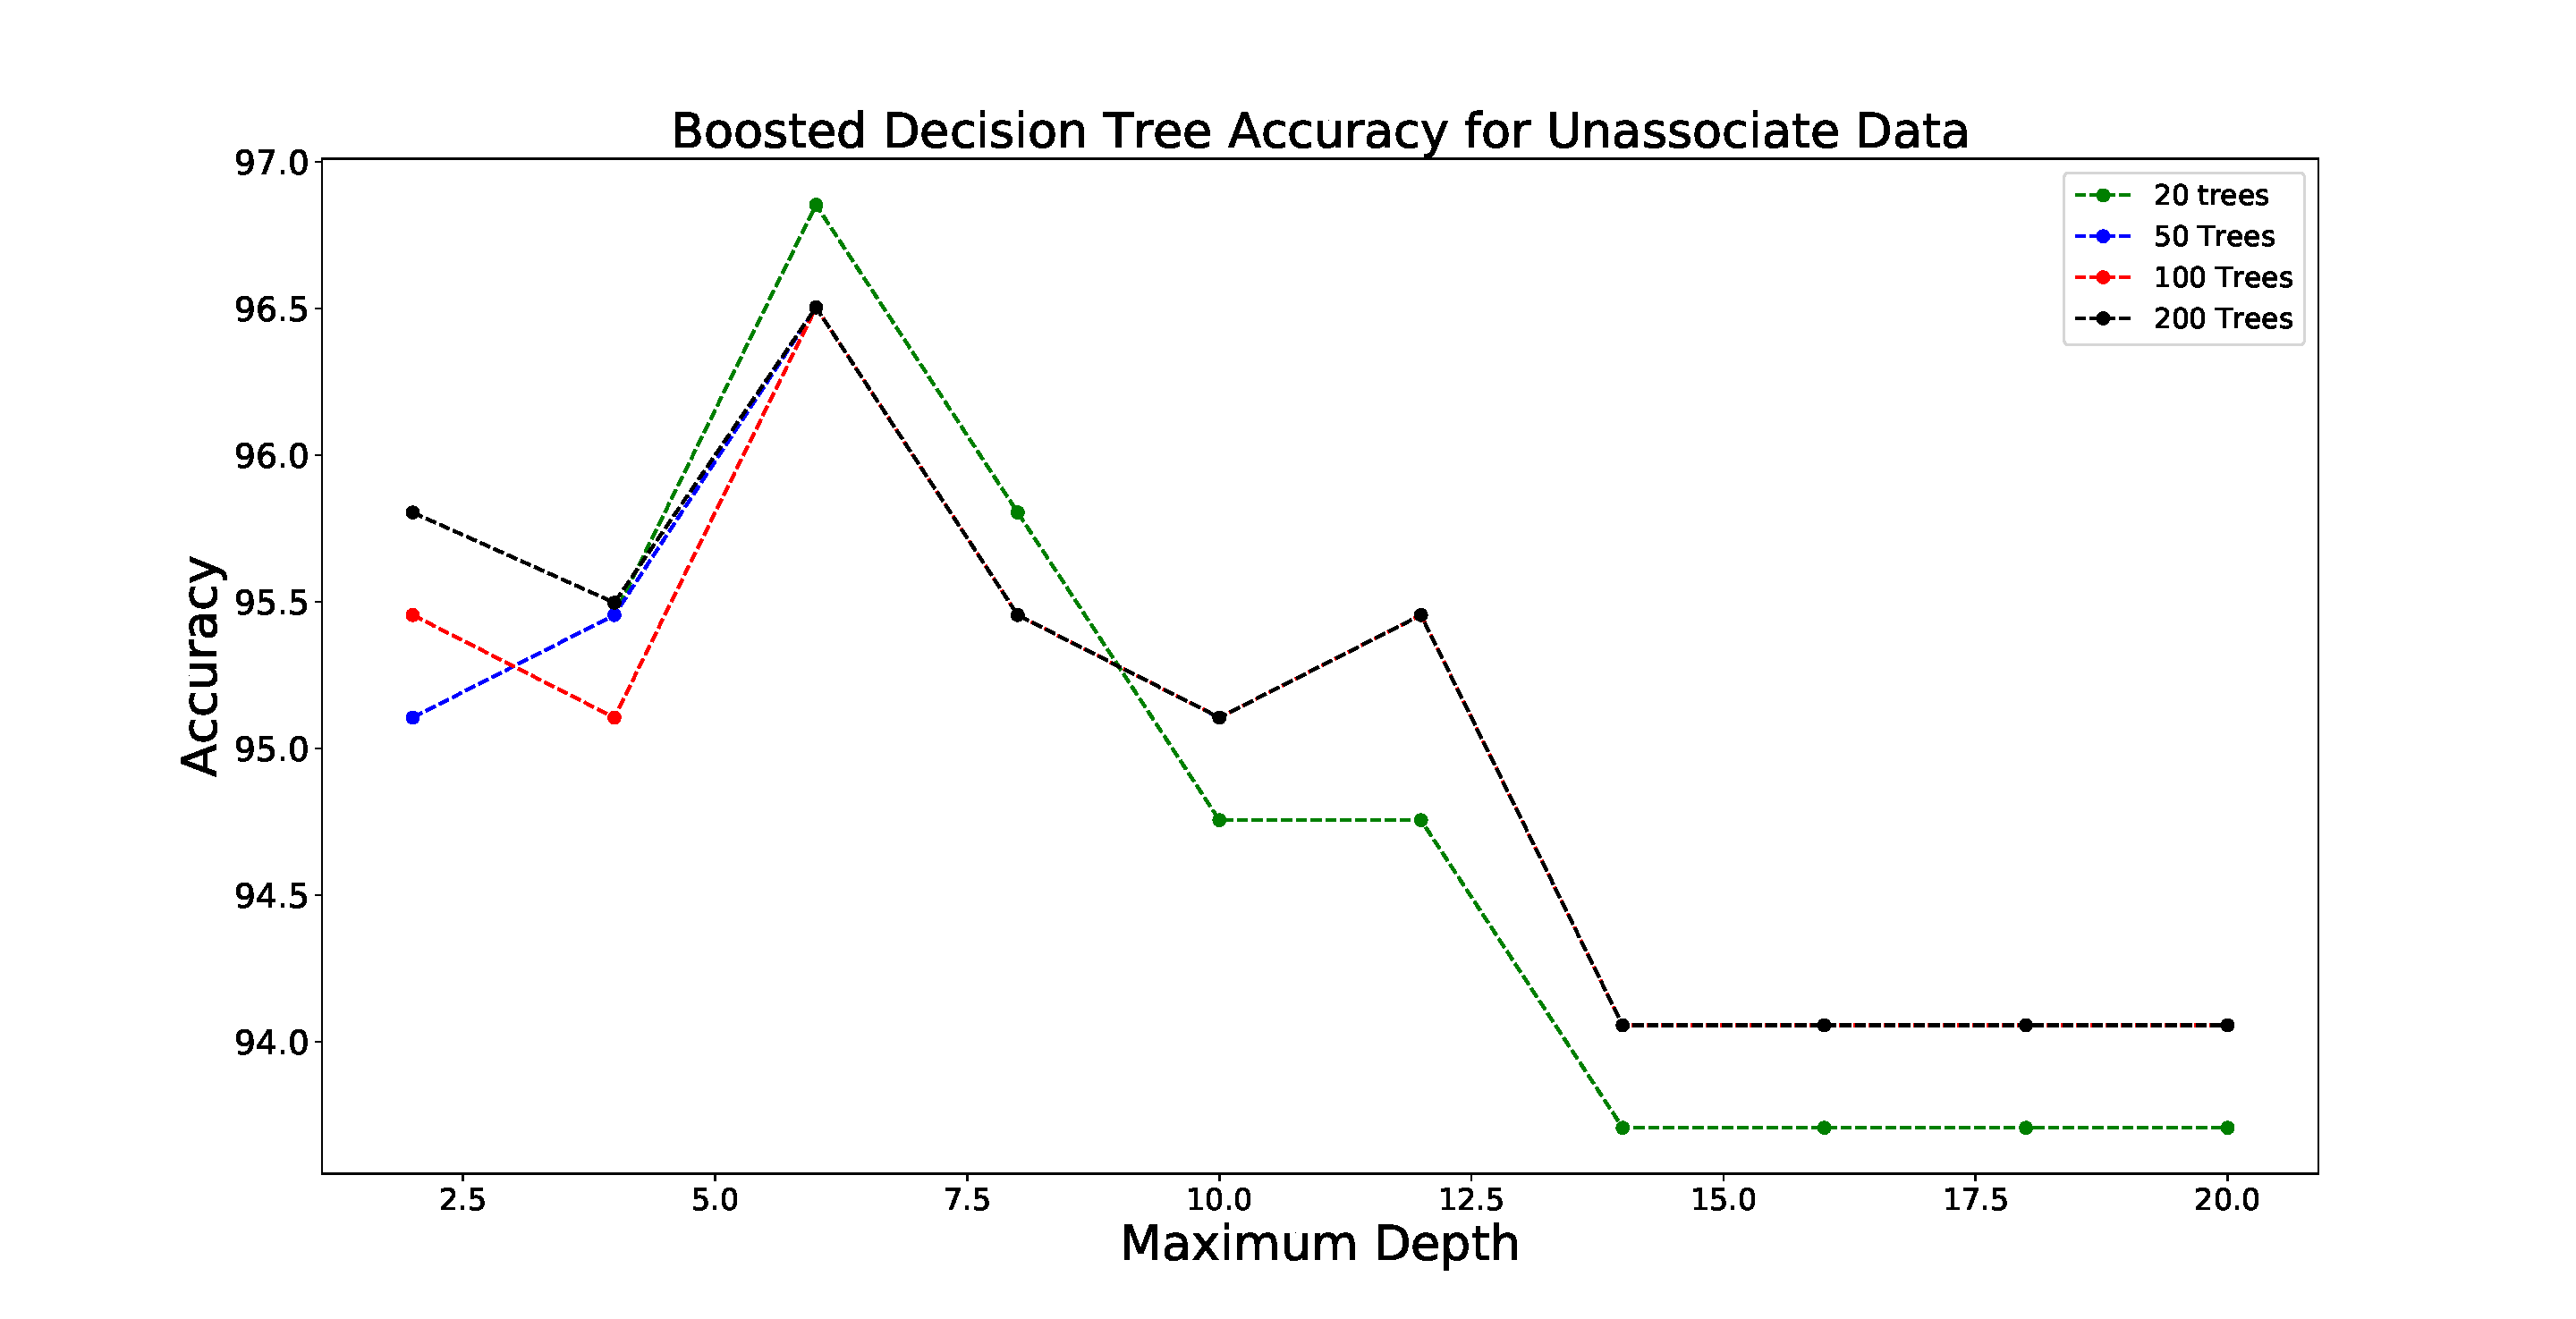
\includegraphics[width=\twopicsp\textwidth]{plots/unassoc_complex.pdf}
\caption{Dependence of LR on tolerance and regularization}
\label{fig:LR_tol_reg}
\end{figure}

In Figure \ref{fig:nn_nn} we show the effect of adding the second hidden layer in the NN algorithm.
The difference between the best accuracies with the additional hidden layer is less then 1\%
compared with the NN with one hidden layer (cf. Table \ref{tab:selected_algs}).
\begin{figure}[h]
%\centerin
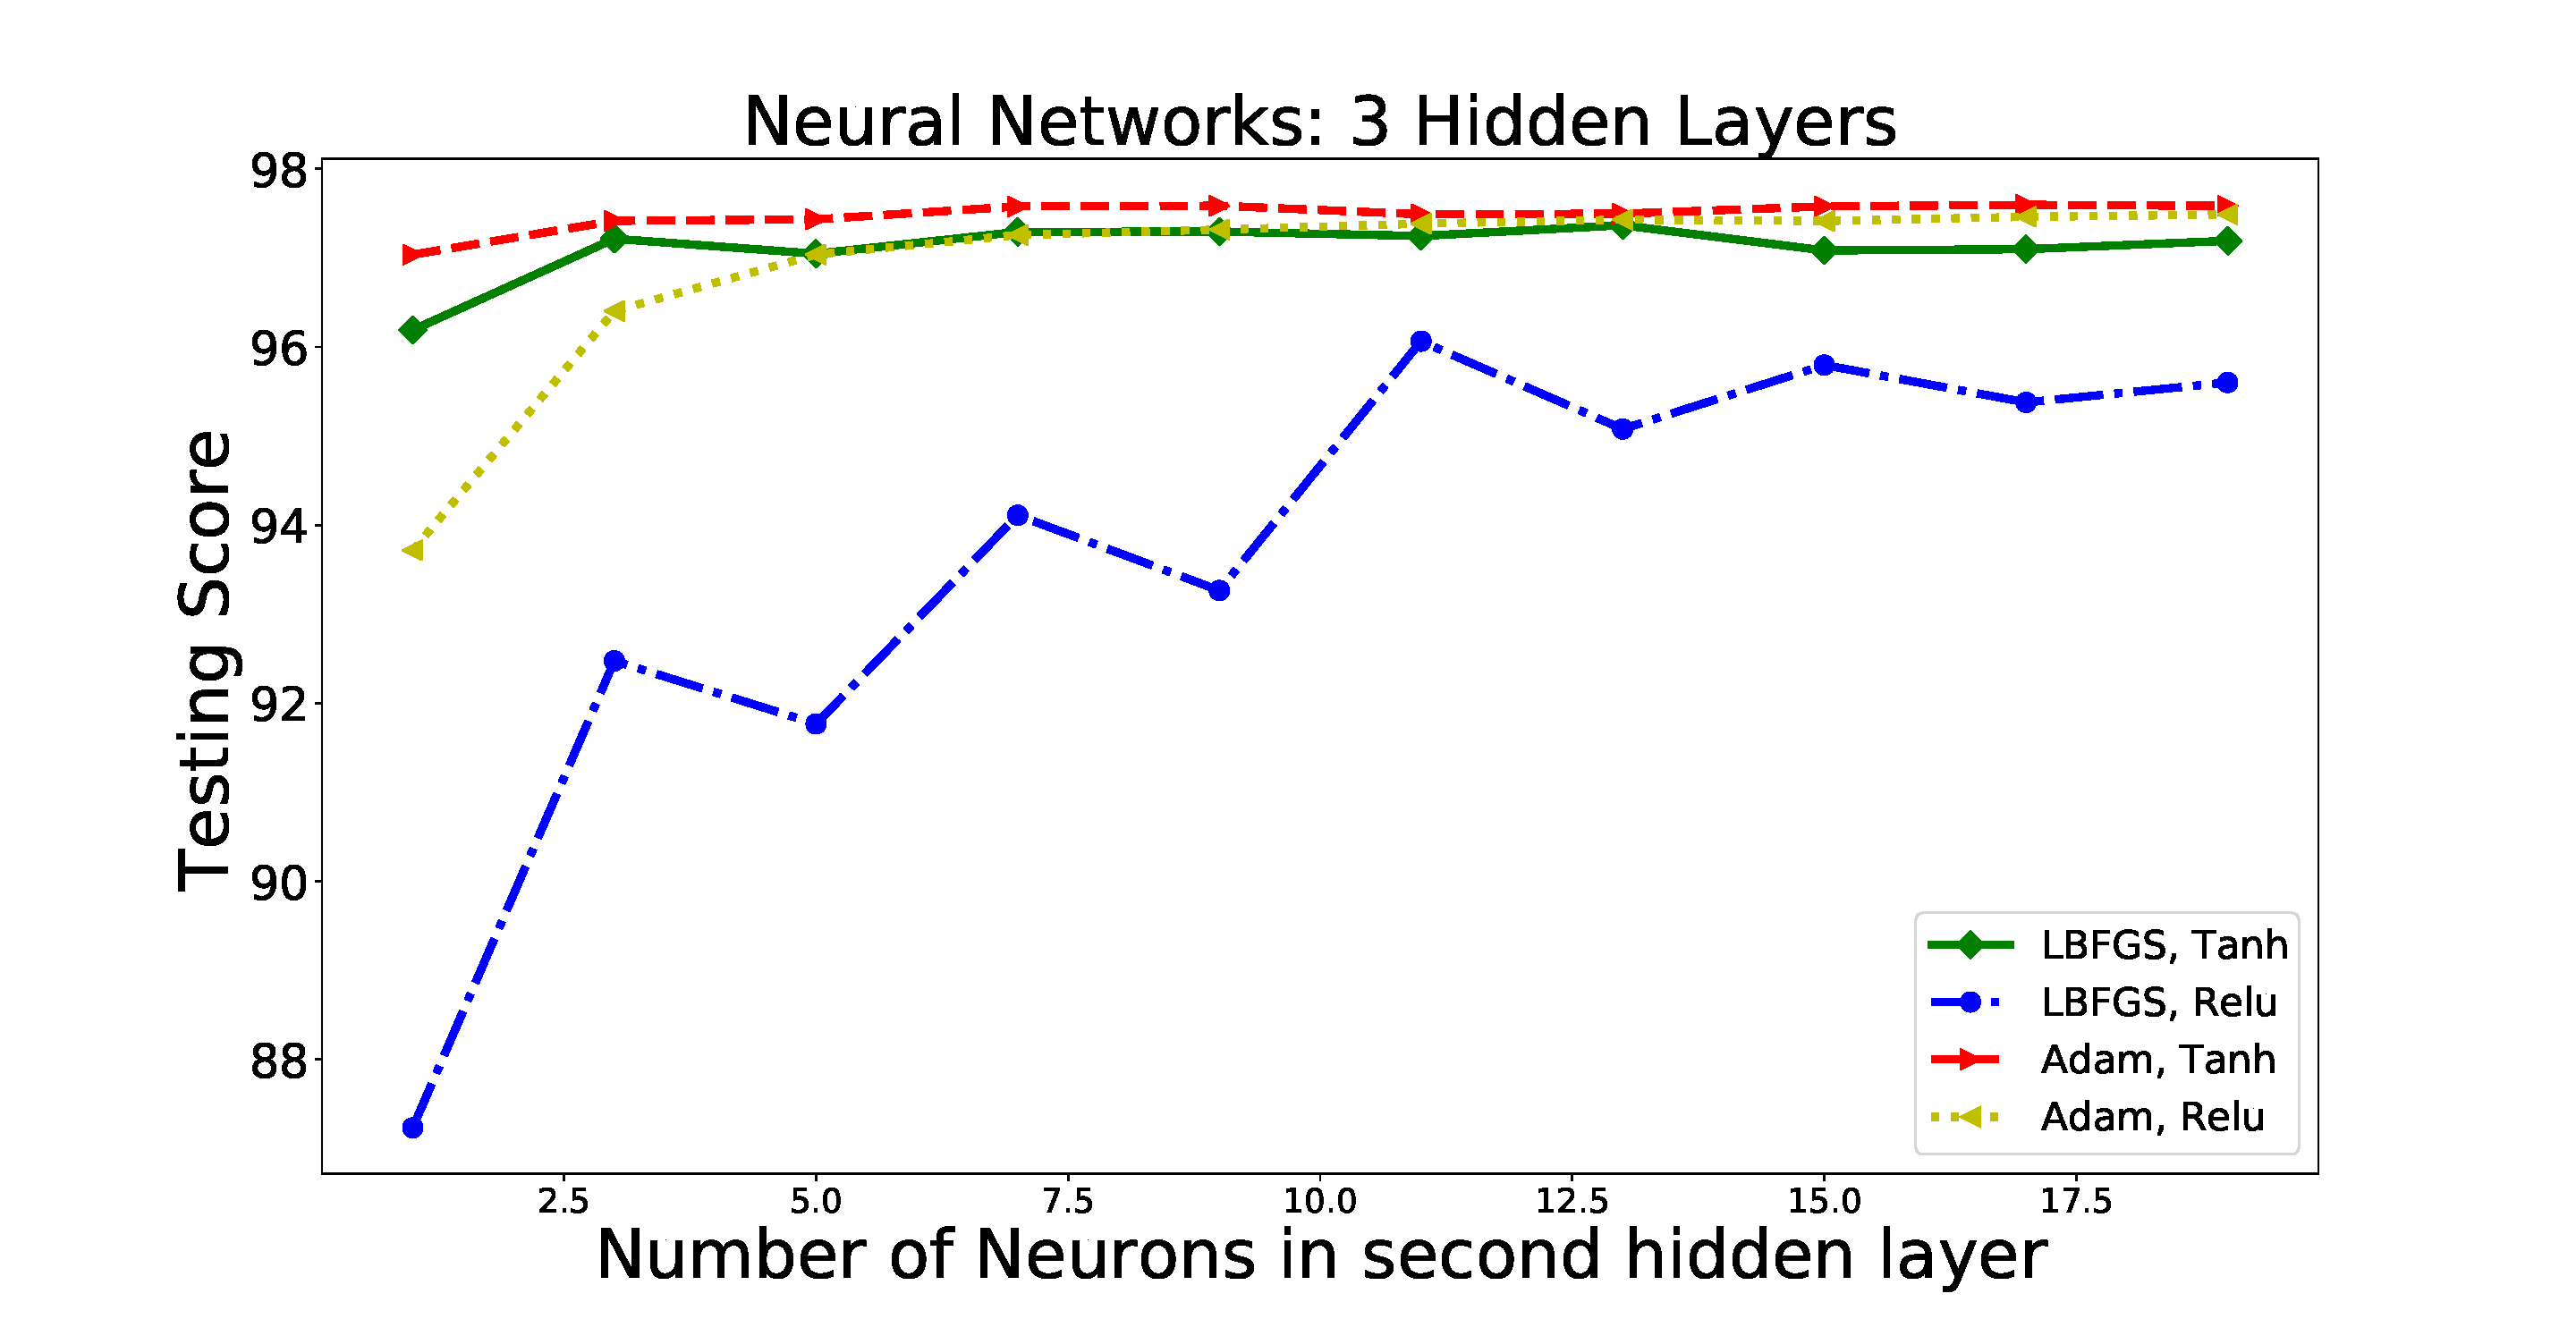
\includegraphics[width=\twopicsp\textwidth]{plots/nn_2layers_3fgl.pdf}
%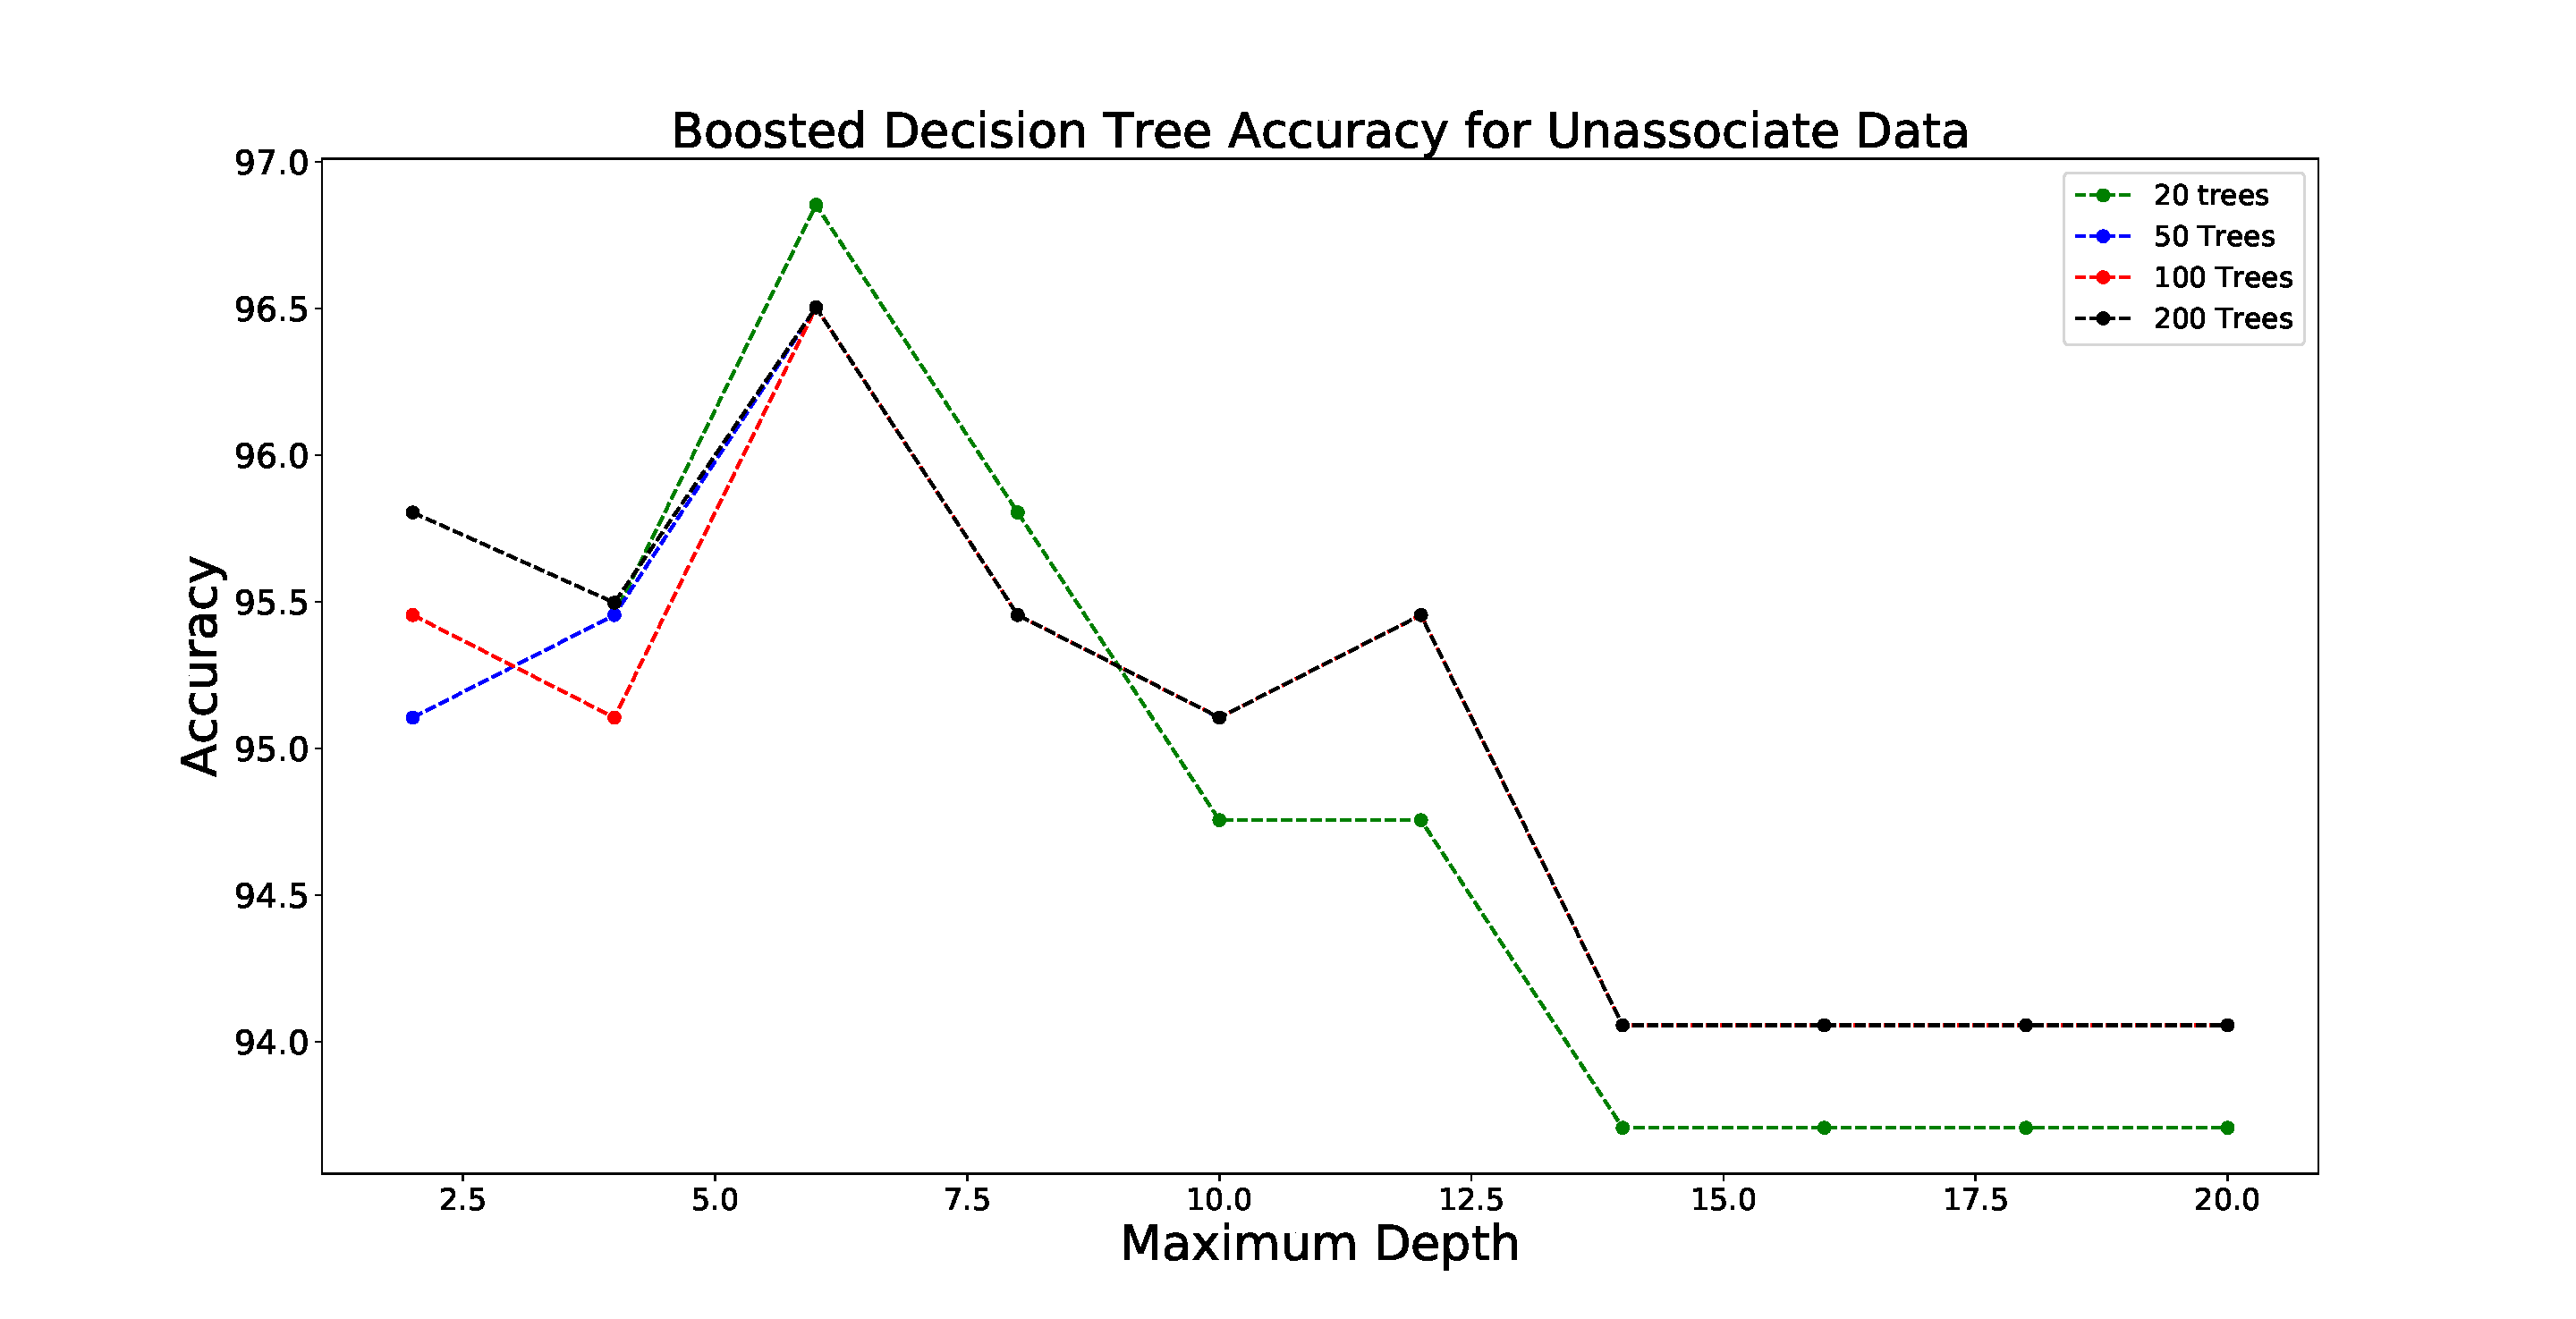
\includegraphics[width=\twopicsp\textwidth]{plots/unassoc_complex.pdf}
\caption{Dependence of NN on the second hidden layer, for 10 neurons in the first layer.}
%\dima{Strictly speaking this is the case of 3 hidden layers.}}
\label{fig:nn_nn}
\end{figure}

At the end we summarize features and their statistics,
which we use for probabilistic classification of sources in the 3FGL and 4FGL catalogs,
in Tables \ref{tab:3FGL_features} and \ref{tab:4FGL_features} respectively. 

\pgfplotstableread[col sep=comma]{tables/features/3fglassocfeaturesAGNPSRnewfeats.csv}\tablea
\begin{table}
\resizebox{0.45\textwidth}{!}{
\pgfplotstabletypeset[
columns={Name,Mean,SD,Minimum,Maximum},
column type=c,
string type,
every head row/.style={before row=\toprule,after row=\midrule,},
every last row/.append style={after row={\hline} },
every first column/.style={column type/.add={|}{}},
every last column/.style={column type/.add={}{|}},
columns/Name/.style={column name=Feature Name,string replace*={_}{\textunderscore}},
columns/Mean/.style={column name=Mean,column type=c,numeric type,fixed,precision=2},
columns/SD/.style={column name=Standard Deviation,numeric type,fixed,precision=2},
columns/Minimum/.style={column name=Minimum,numeric type,fixed,precision=2},
columns/Maximum/.style={column name=Maximum,numeric type,fixed,precision=2},
skip rows between index={11}{25}
]{\tablea}
}
\vspace{0.2cm}
\caption{Statistics of features used for 2 class probabilistic classification of the 3FGL sources.
\lb{tab:3FGL_features}}
\end{table}

\pgfplotstableread[col sep=comma]{tables/features/4fglassocfeatures.csv}\tableaf
\begin{table}
\resizebox{0.45\textwidth}{!}{
\pgfplotstabletypeset[
columns={Name,Mean,SD,Minimum,Maximum},
column type=c,
string type,
every head row/.style={before row=\toprule,after row=\midrule,},
every last row/.append style={after row={\hline} },
every first column/.style={column type/.add={|}{}},
every last column/.style={column type/.add={}{|}},
columns/Name/.style={column name=Feature Name,string replace*={_}{\textunderscore}},
columns/Mean/.style={column name=Mean,column type=c,numeric type,fixed,precision=2},
columns/SD/.style={column name=Standard Deviation,numeric type,fixed,precision=2},
columns/Minimum/.style={column name=Minimum,numeric type,fixed,precision=2},
columns/Maximum/.style={column name=Maximum,numeric type,fixed,precision=2},
%skip rows between index={17}{28}
]{\tableaf}
}
\vspace{0.2cm}
\caption{Statistics of features used for probabilistic classification of the 4FGL sources.
\lb{tab:4FGL_features}}
\end{table}




\end{appendix}

\end{document}

